% Comment R2 - 1 

\begin{spacing}{1}
\justifying \color{darkdarkgray} \noindent

Thank you very much for your careful and critical feedback, which has substantially strengthened the paper. In particular, your concern about spatial spillovers was particularly useful: following your suggestions, we developed a new set of empirical exercises---summarized in a new Section 4.2 and detailed in Online Appendix C---that directly test for the displacement of crime and police resources to neighboring municipalities. Your comment on the institutional context of \emph{Plan Cuadrante} was equally valuable and led us to substantially expand Section 2. We have carefully considered all your comments and hope that we adequately addressed them in the revised manuscript and in the response document below.


\end{spacing}


\begin{bibunit}


\begin{refcomment}

Framing of the paper: Section 2 lacks sufficient details on the design and implementation of “Plan Cuadrante”. In particular, I would like to see more information on the resources involved (e.g., number of officers, cars, etc.) and the rules or criteria for their allocation across quadrants and municipalities. This would not only strengthen the reader’s understanding of the intervention but also help in evaluating the plausibility of the proposed mechanisms.
\label{pt:r2_01}

\end{refcomment}


\begin{response}
    %Regarding my main concern---spillovers---the current version is considerably more transparent, and Section 4.2, together with the Online Appendix, attempts to address this threat to identification. I would, however, encourage the authors to reorganize the presentation of this evidence. My suggestion would be to lead with the exposure-based specification, in which exposure to treated neighbors is measured continuously. In my view, this is the most informative of the three exercises because it exploits variation in the intensity of potential spillovers rather than relying on a binary indicator for having a treated neighbor. This specification should, of course, be presented with the appropriate caveat: exposure to treated neighbors is not randomly assigned, so the estimates do not fully address the possibility that municipalities with many early-adopting neighbors differ systematically in other respects.


Thanks. We have reorganized the presentation of the evidence on spillovers, as suggested. Section 4.2 now leads with the exposure-based specification following \citet{crepon2013}, which measures exposure to treated neighbors continuously (as the share and the number of treated neighbors), and only then presents the binary neighbor-treatment specification. As you note, the exposure-based specification is the more informative of the two, since it exploits variation in the intensity of potential spillovers rather than relying on a binary indicator for having a treated neighbor.

When commenting on the results of the exposure-based specification, we have introduced the recommended caveat, which now reads as follows in the paper: ``Because exposure to treated neighbors is not randomly assigned, however, this evidence does not fully rule out the possibility that municipalities with many early-adopting neighbors differ systematically from those with fewer such neighbors in other respects that are also correlated with our outcomes.''

Separately, and to keep the spillovers discussion focused, we have also removed the randomization-inference exercise from this section, since (as discussed in our response to your next comment) it is better understood as a general robustness check on our main estimates than as a targeted test for spillovers. We now report it separately when discussing our main results, with the full exercise moved to its own subsection in the Online Appendix (Section C.8).
\end{response}
\stepcounter{AnsweredComments}




\begin{refcomment}

Data: Chile has around 350 municipalities, yet the main analysis uses survey data for only 46 urban municipalities after excluding “always treated” municipalities. This restricted sample raises questions about external validity and potential biases: To what extent might this selection affect the results? Are these 46 municipalities spatially clustered or connected in ways that could bias comparisons? Could omitted municipalities differ systematically in crime dynamics or socio-economic characteristics? All these issues deserve some discussion in the paper.

\label{pt:r2_02}
\end{refcomment}


\begin{response}
    %I also had difficulty following the randomization-inference exercise for spillovers. This may simply reflect my own misunderstanding, but although I understand randomization inference in general, the purpose of this particular exercise as a test for spillovers was unclear to me. It may therefore warrant further explanation. In particular, how does the exercise help address concerns about spillovers? Why is treatment status reshuffled across all 346 municipalities when significantly fewer municipalities were ever eligible for the program?



\end{response}
\stepcounter{AnsweredComments}


% Comment R2 - 3 
\begin{refcomment}

\smallskip

Methods and Results: My main concern relates to SUTVA violations due to spillovers.

Control municipalities may be indirectly affected by the implementation of “Plan Cuadrante” in treated municipalities, which could bias the ATT estimates. Two channels seem particularly relevant: a) Crime displacement (criminal activity might shift from treated to nearby untreated municipalities) and b) Resource displacement (personnel, vehicles, or budget may have been diverted from control to treated municipalities).

Unfortunately, the robustness check used by the authors to claim “no spillovers” to neighboring untreated municipalities is only briefly mentioned in Section 3.2. Having read the appendix looking for details, I still have two concerns about their exercise. First, given that the main ENUSC sample includes only 46 municipalities, it is unclear which municipalities are considered “neighboring municipalities” in this test (i.e., how many neighbor municipalities do you have among the 46 municipalities considered?). Second, identifying spatial spillovers generally requires more sophisticated designs such as two-stage randomization as in Crépon et al. (2013) in the context of labor markets, or Blattman et al. (2021) in the context of crime. Thus, it is unclear to what extent the current exercise can capture spillovers. A revised version of the paper should include a more serious discussion of this issue in the main body of the paper.

\label{pt:r2_03}
\end{refcomment}

\begin{response}
    %% Comment 3: Methods and Results: My main concern relates to SUTVA violations due to spillovers.

%Control municipalities may be indirectly affected by the implementation of “Plan Cuadrante” in treated municipalities, which could bias the ATT estimates. Two channels seem particularly relevant: a) Crime displacement (criminal activity might shift from treated to nearby untreated municipalities) and b) Resource displacement (personnel, vehicles, or budget may have been diverted from control to treated municipalities).

%Unfortunately, the robustness check used by the authors to claim “no spillovers” to neighboring untreated municipalities is only briefly mentioned in Section 3.2. Having read the appendix looking for details, I still have two concerns about their exercise. First, given that the main ENUSC sample includes only 46 municipalities, it is unclear which municipalities are considered “neighboring municipalities” in this test (i.e., how many neighbor municipalities do you have among the 46 municipalities considered?). Second, identifying spatial spillovers generally requires more sophisticated designs such as two-stage randomization as in Crépon et al. (2013) in the context of labor markets, or Blattman et al. (2021) in the context of crime. Thus, it is unclear to what extent the current exercise can capture spillovers. A revised version of the paper should include a more serious discussion of this issue in the main body of the paper.

Thank you very much for the feedback around spillovers, which we agree was crucial and did not receive the necessary attention in the previous version of the manuscript.

Spillovers from treated municipalities to control municipalities can bias the estimates upwards for two reasons. First, \emph{Plan Cuadrante} might displace criminals from committing crime in treatment municipalities to committing crime in control municipalities. Second, the program could in principle relocate police resources from nearby control municipalities to treated ones. In the revised manuscript, we address both channels directly. We first use administrative data on reported crime and arrests, which are available since 2002 for crime and since 2005 for arrests for all Chilean municipalities, rather than being restricted to the 47 municipalities surveyed in ENUSC. These administrative samples include 292 municipalities for reported crime and 281 for arrests, out of a total of 346 municipalities.\footnote{The municipalities excluded from these samples are the always-treated municipalities, which adopted \emph{Plan Cuadrante} before the administrative data begin.} The results, presented in the appendix and summarized in the new spillovers section of the main text, show no evidence that \emph{Plan Cuadrante} displaced crime or arrests to nearby untreated municipalities.

We then expand the analysis to police resources, again finding no meaningful spillovers. This is consistent with the institutional functioning of Carabineros. Transfers of uniformed officers are difficult outside the 10-year service period in each location, and the program documents indicate that the resource increases associated with \emph{Plan Cuadrante} were driven mainly by new hirings rather than by reallocating officers or vehicles from control to treatment areas. This is also consistent with the fact that police resources increased substantially in both treatment and control municipalities during the 2000s and 2010s.

We also examine the 46 ENUSC municipalities separately. Even in that smaller sample, where the potential for spillovers is harder to assess, we find no evidence that early adopters displaced crime or resources onto later adopters before those municipalities themselves joined the program.

Following your suggestion, we further conduct two additional exercises. First, following \citet{crepon2013}, we estimate the effect of a higher share of neighboring municipalities adopting \emph{Plan Cuadrante} on crime, arrests, and police resources in control municipalities, finding no significant effects on any of these outcomes. Second, following \citet{Blattman}, we implement a randomization inference exercise in which treatment status and adoption dates are randomly assigned 1,000 times, constructing placebo distributions of treatment and spillover effects. The true treatment effect on crime falls in the bottom 1\% of the placebo distribution, while the estimated spillover effects fall within the 40th--45th percentile, providing no evidence of meaningful spillovers on crime, arrests, or resources onto neighboring untreated municipalities.

Finally, the broad administrative coverage allows us to estimate spillovers credibly using the full set of administrative outcomes, while the ENUSC outcomes are more limited because only 46 adopting municipalities and 1 never-treated municipality are observed. Within ENUSC, only 10 municipalities share a border with another municipality surveyed in ENUSC, and only 6 share a border with either a never-treated municipality or a treated municipality that adopted the program in a different year. We therefore rely on the administrative exercises for the main spillover evidence and use the ENUSC subsample as a complementary check.


We are providing below the new section added to the manuscript summarizing the results of the spillover analyses and the Appendix providing the details of the spillover analyses:\\ 

\begin{adjustwidth}{2em}{0em}
%\textbf{4.2 \emph{Plan Cuadrante} and Spatial Spillovers}

Beyond parallel trends, a causal interpretation of our estimates requires the absence of spillover effects from treated to control municipalities, since such spillovers could bias treatment effects upward. This concern is relevant in our setting. Previous work on deployment-based policing reforms, such as hot-spot policing, shows that crime may be displaced to nearby areas \citep{Blattman_Tobon_JEEA}. Spillovers could also arise through the reallocation of police resources from control to treated municipalities.

In our setting, spillovers are less likely for several reasons. First, as discussed in Section \ref{institutions}, \emph{Plan Cuadrante} introduced beat policing in Chile by reorganizing deployment across the full municipal territory rather than concentrating resources in specific hot spots. Second, Chilean municipalities are large---on average 101,000 inhabitants and 2,000 square kilometers \citep{SINIM}---and criminals typically do not travel such long distances to commit crimes, which makes displacement to other municipalities unlikely \citep{Langella}. Third, and more directly related to police resources, police regulations assign officers to \emph{comisar\'ias}---broader operational units that usually cover an entire municipality---for fixed periods, which limits rapid reallocation of officers across jurisdictions.\footnote{See the Transfer Manual for Carabineros de Chile Personnel available at \url{https://www.carabineros.cl/transparencia/og/pdf/OG_2707_13112019.pdf}}

We nonetheless assess spillovers empirically through two complementary exercises using administrative data at the national level. Online Appendix \ref{sec:appendixC} reports the full results. First, following \citet{crepon2013}, we test whether higher exposure to \emph{Plan Cuadrante} among neighboring municipalities affects outcomes in control municipalities. Online Appendix Figures \ref{fig:figure_continuous_spillovers} and \ref{fig:figure_count_spillovers}---which define neighbor exposure as the share and the number of treated neighbors, respectively---show no meaningful effects across the outcomes we study, suggesting the absence of spatial spillovers. Because exposure to treated neighbors is not randomly assigned, however, this evidence does not fully rule out the possibility that municipalities with many early-adopting neighbors differ systematically from those with fewer such neighbors in other respects that are also correlated with our outcomes.

Second, we estimate the effect of \emph{Plan Cuadrante} on police-reported crime and police resources in untreated municipalities whose neighbors adopt the program. Online Appendix Figure \ref{fig:spillover_admin} summarizes these estimates and again shows no evidence of spatial spillovers.

The exercises above evaluate spatial spillovers using administrative records for the extended municipality sample. We complement this evidence with two additional analyses focused on ENUSC municipalities. First, we re-estimate the administrative-outcome spillover analysis---for reported crime, arrests, police officers, and patrol vehicles---restricting the sample to neighbors of the 46 ENUSC municipalities (Online Appendix Figure \ref{fig:figure_46ENUSC_spillovers_admin}). Second, we test for spillovers directly in ENUSC outcomes. Because ENUSC coverage is limited---46 treated municipalities and 1 never-treated municipality, with only 10 sharing a border and 6 of those treated in different years---we estimate spillover effects from early-adopting ENUSC municipalities onto late-adopting ENUSC neighbors before the latter adopt the program (Online Appendix Figure \ref{fig:figure_results_spillovers_enusc}). Both exercises yield reassuringly null effects.

Taken together, these results indicate that spatial spillovers are unlikely to threaten identification in our setting.

\FloatBarrier
\end{adjustwidth}


\begin{adjustwidth}{2em}{0em}
This Online Appendix details the specifications behind the spillover tests summarized in Section~\ref{sec:spillovers}.

The baseline test estimates the effect of \emph{Plan Cuadrante} on reported crime, arrests, police officers, and patrol vehicles in neighboring untreated municipalities,
\begin{equation}
Outcome_{mt}= \delta_{1}\,\mbox{\textit{Plan Cuadrante near municip.}}_{mt} + Municipality_{m} + Year_{t} + u_{mt}
\label{eq:main3}
\end{equation}
\noindent where the sample is restricted to municipalities that never adopted the program, each is assigned a treatment date equal to the earliest adoption among its treated neighbors, and $\delta_{1}$ is estimated dynamically with the staggered difference-in-differences estimator of \citet{Callaway}. Because these administrative outcomes are observed for every municipality, we estimate the specification on the full national sample of never treated municipalities (Online Appendix Figure~\ref{fig:spillover_admin}).

For the intensity-based test in the spirit of \citet{crepon2013}, we replace the binary neighbor-treatment indicator with a continuous measure of exposure and restrict the sample to never-treated municipalities,
\begin{equation}
Outcome_{mt}= \delta_{1}\,\mbox{\textit{Share neighbors with Plan Cuadrante}}_{mt} + Municipality_{m} + Year_{t} + u_{mt}
\label{eq:crepon}
\end{equation}
\noindent Because the treatment is continuous, we estimate it with the heterogeneity-robust estimator of \citet{Chaisemartin}, measuring exposure both as the share of treated neighbors (Online Appendix Figure~\ref{fig:figure_continuous_spillovers}) and as their number (Online Appendix Figure~\ref{fig:figure_count_spillovers}).

For the randomization-inference test, we reassign adoption dates and never-treated status across municipalities $1{,}000$ times and re-estimate the direct and spillover effects under the sharp null, yielding the placebo distributions in Online Appendix Figure~\ref{fig:ri_placebo}. For this exercise we rely on the estimator of \citet{Chaisemartin} rather than that of \citet{Callaway}: re-estimating the latter over a thousand permutations would require prohibitive computational power and running time.

Finally, we re-estimate the baseline administrative specification on the municipalities neighboring the 46 ENUSC municipalities (Online Appendix Figure~\ref{fig:figure_46ENUSC_spillovers_admin}); and, for the outcomes measured only in ENUSC, we estimate the spillover of early-adopting ENUSC municipalities on their late-adopting ENUSC neighbors before the latter's own adoption (Online Appendix Figure~\ref{fig:figure_results_spillovers_enusc}). The six focal late-adopters, each shown with its earliest-adopting ENUSC neighbor and that neighbor's adoption year, are Molina (Curic\'o, 2005), Tocopilla (Iquique, 2005), San Carlos (Chill\'an, 2007), Padre Hurtado (Pe\~naflor, 2008), Calera (Quillota, 2008), and Limache (Quillota, 2008). Across all of these specifications, the estimated spillover effects are small and statistically indistinguishable from zero.

\end{adjustwidth}

\clearpage
\noindent\textbf{Other figures and tables referenced above:}
\vspace{0.5em}

{\renewcommand{\thefigure}{C.12}
%--- Implementation
\begin{figure}[h!]
    \centering
    \caption{Geographic Spillovers of \emph{Plan Cuadrante} on Neighboring Untreated Municipalities}
    \label{fig:spillover_admin}
    \begin{subfigure}{0.495\textwidth}
        \centering
        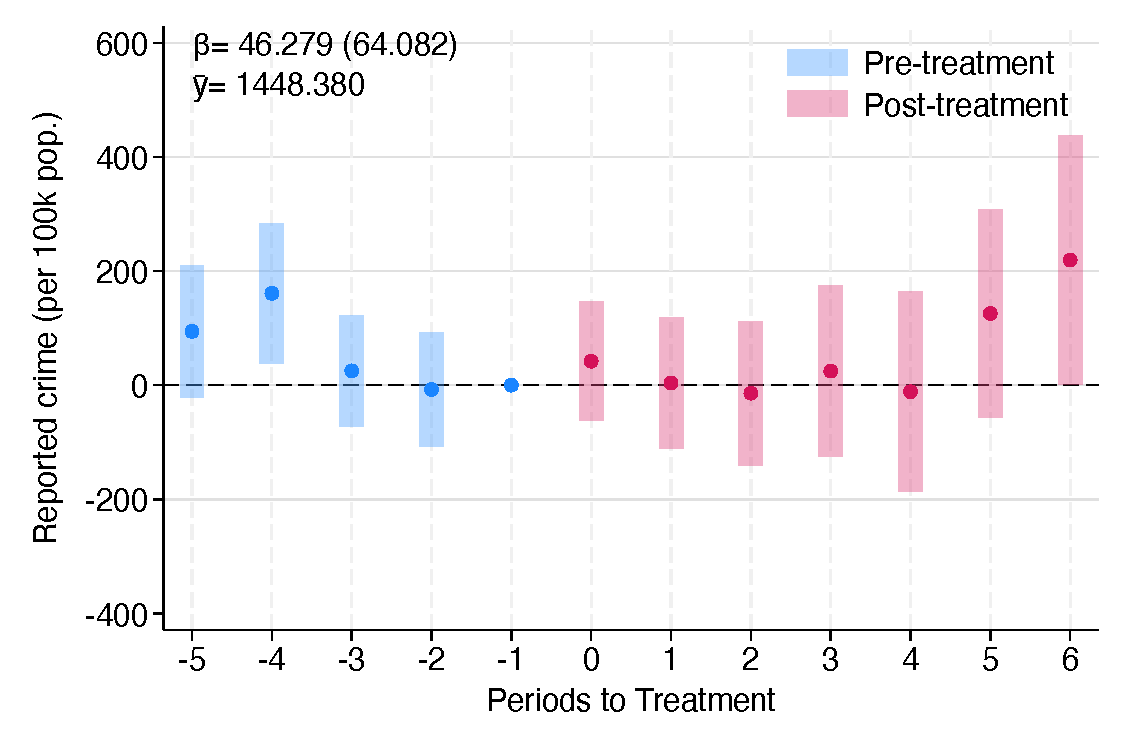
\includegraphics[width=0.98\textwidth]{../manuscript/Graphs/totalreportedcrime_allcomunas_neighbors.pdf}
        \caption{Spillovers on Reported crime}
    \end{subfigure}%
    ~ 
    \begin{subfigure}{0.495\textwidth}
    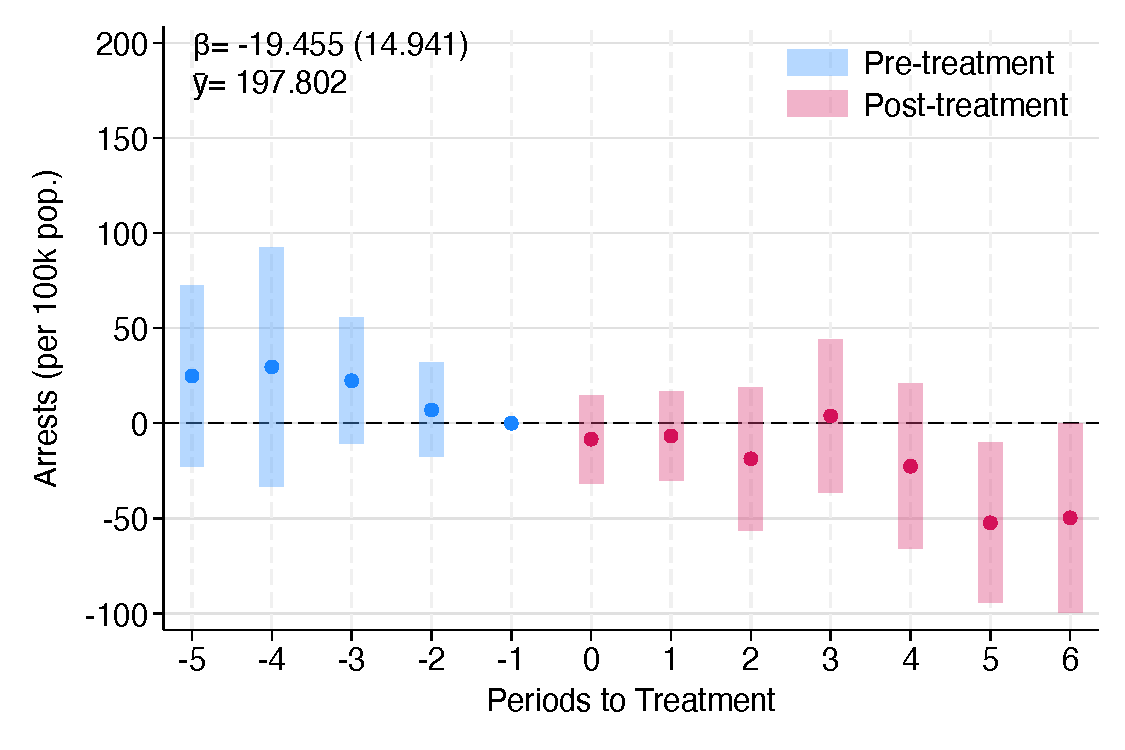
\includegraphics[width=0.98\textwidth]{../manuscript/Graphs/totalarrestscrime_allcomunas_neighbors.pdf}
        \caption{Spillovers on Arrests}
    \end{subfigure}
    \begin{subfigure}{0.495\textwidth}
        \centering
        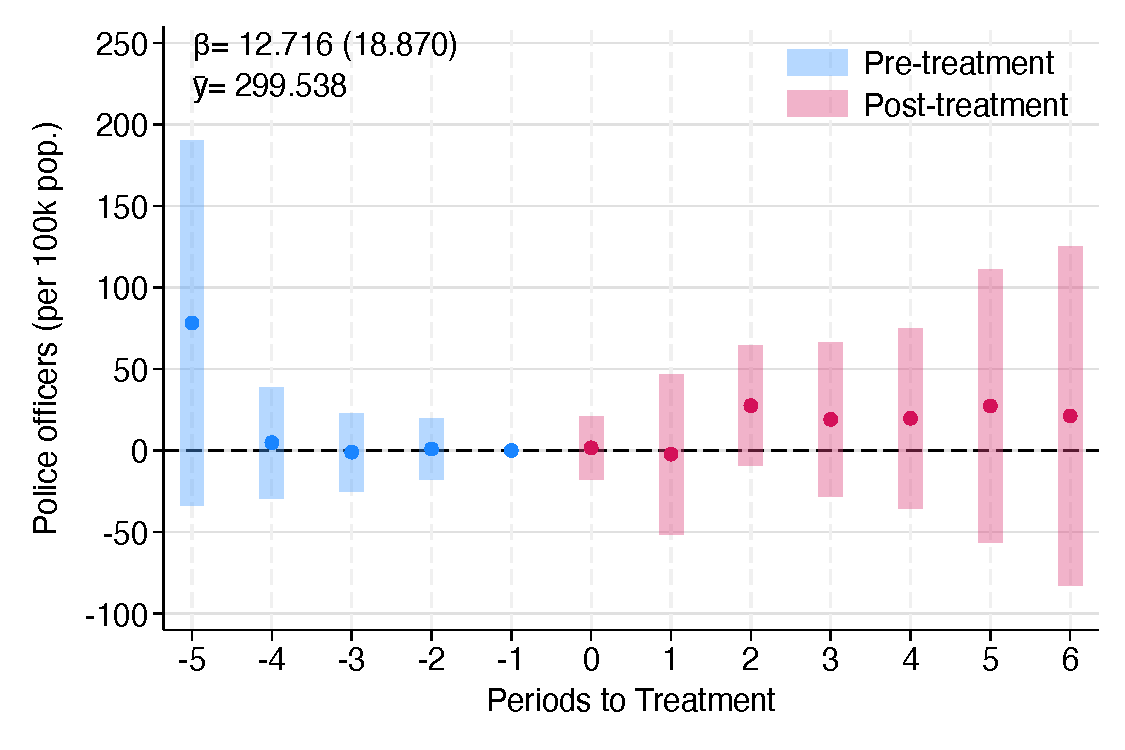
\includegraphics[width=0.98\textwidth]{../manuscript/Graphs/dotpc_allcomunas_neighbors.pdf}
        \caption{Spillovers on Police Officers}
    \end{subfigure}%
    ~ 
    \begin{subfigure}{0.495\textwidth}
    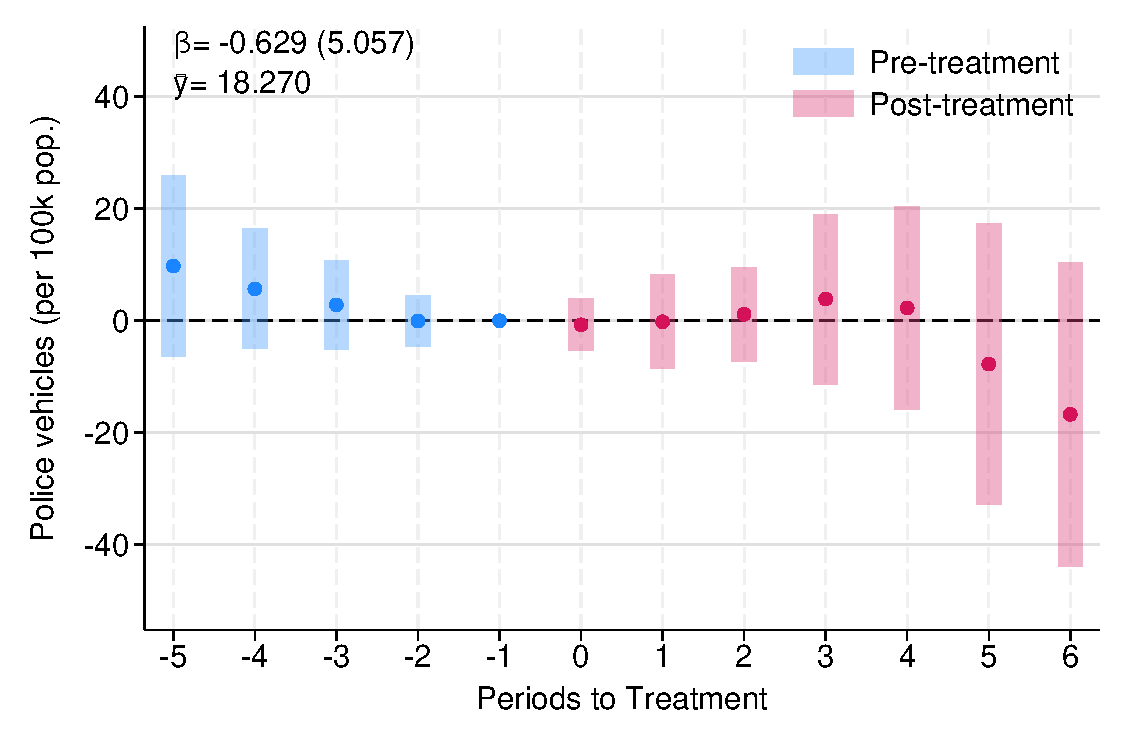
\includegraphics[width=0.98\textwidth]{../manuscript/Graphs/vehiclespc_allcomunas_neighbors.pdf}
        \caption{Spillovers on Patrol Vehicles}
    \end{subfigure}
    \begin{minipage}{0.9\textwidth}
    \footnotesize
    Notes: This figure reports the spillover effects of \emph{Plan Cuadrante} on the number of crimes reported to the police in the municipality per 100,000 inhabitants (panel a), the number of arrests in the municipality per 100,000 inhabitants (panel b), the number of police officers per 100,000 inhabitants (panel c), and the number of patrol vehicles per 100,000 inhabitants (panel d). Panels (a)--(d) include 2,859, 2,166, 1,144, and 1,942 observations respectively. Specifically, the figure shows the dynamic effects of the \emph{Plan Cuadrante} for neighbor municipalities which never introduced the program. The estimation is conducted using the procedure developed in \citet{Callaway} for difference-in-differences with staggered treatment adoption, using as the treatment introduction date the earliest date of a neighboring municipality. The dots in the figure represent the estimated coefficients and the bars behind them 95\% confidence intervals. Standard errors are clustered at the municipality level using the wild bootstrapping procedure. The pooled effect and the mean outcome before the introduction of the treatment for every outcome is also presented in each panel. 
    \end{minipage}
\end{figure}
}

\clearpage

{\setcounter{figure}{12}\renewcommand{\thefigure}{C.\arabic{figure}}
\begin{figure}[h!]
    \centering
    \caption{Geographic Spillovers of \emph{Plan Cuadrante} by Share of Treated Neighbors}
    \label{fig:figure_continuous_spillovers}
    \begin{subfigure}{0.495\textwidth}
        \centering
        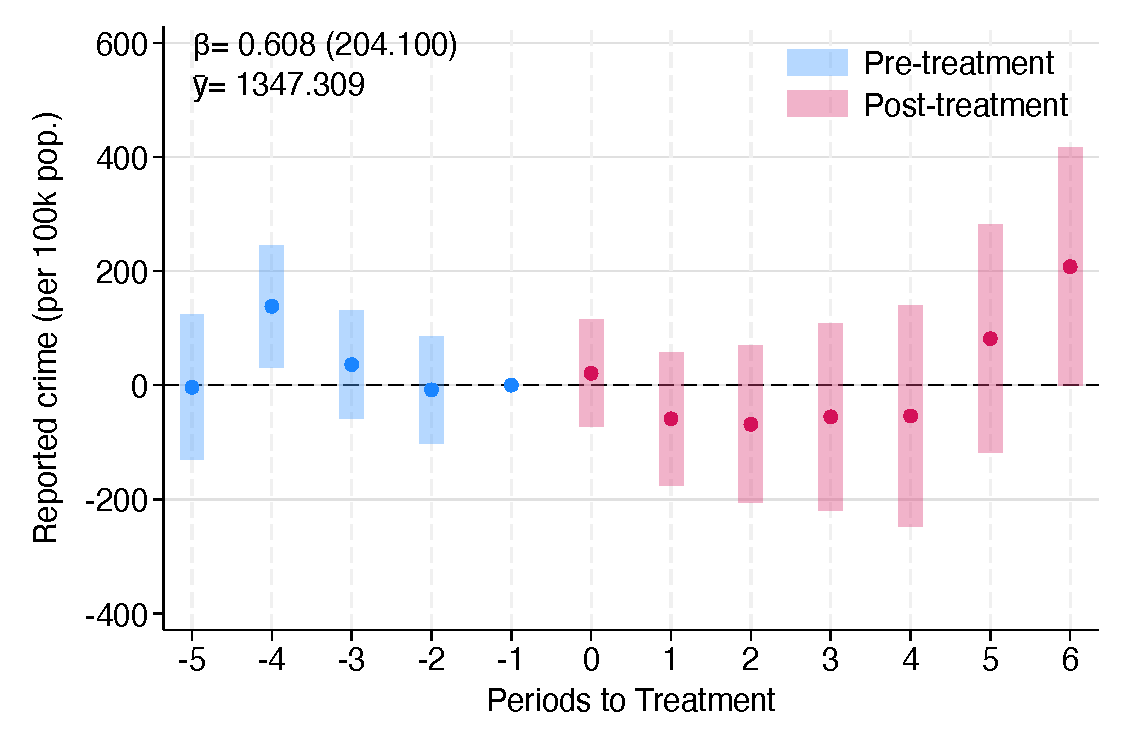
\includegraphics[width=0.98\textwidth]{../manuscript/Graphs/CHDH_continuous_spillover_crime.pdf}
        \caption{Spillovers on Reported Crime}
    \end{subfigure}%
    ~
    \begin{subfigure}{0.495\textwidth}
        \centering
        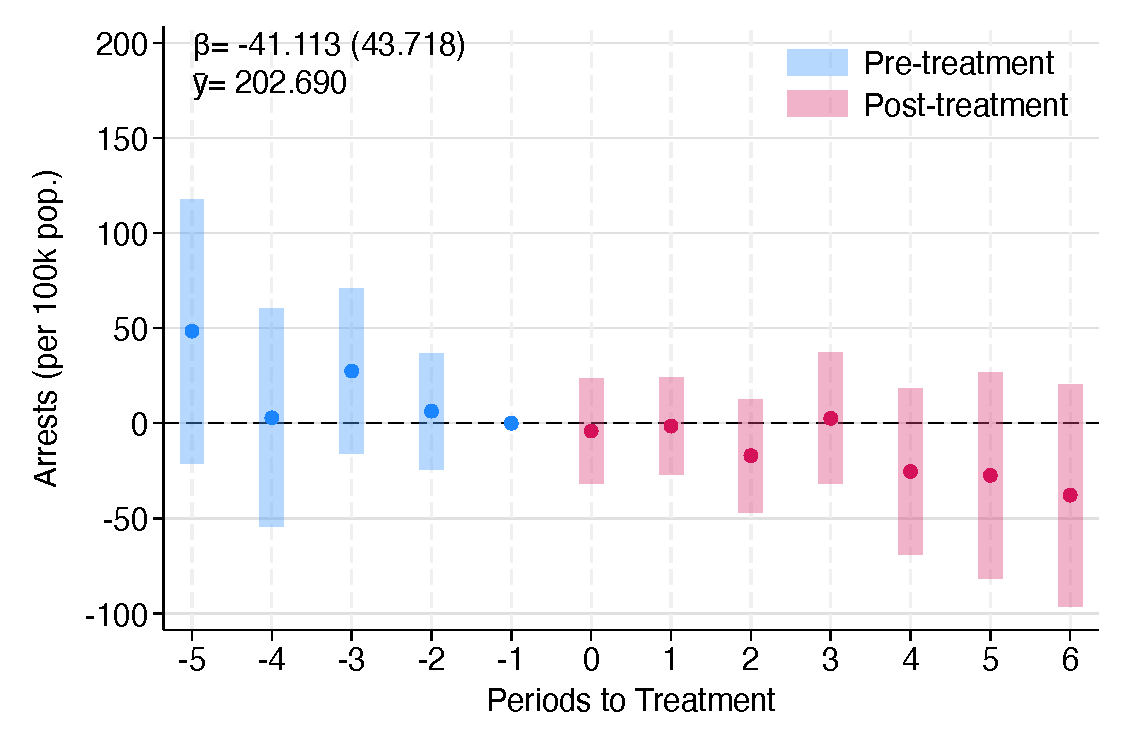
\includegraphics[width=0.98\textwidth]{../manuscript/Graphs/CHDH_continuous_spillover_arrests.pdf}
        \caption{Spillovers on Arrests}
    \end{subfigure}

    \vspace{0.5em}

    \begin{subfigure}{0.495\textwidth}
        \centering
        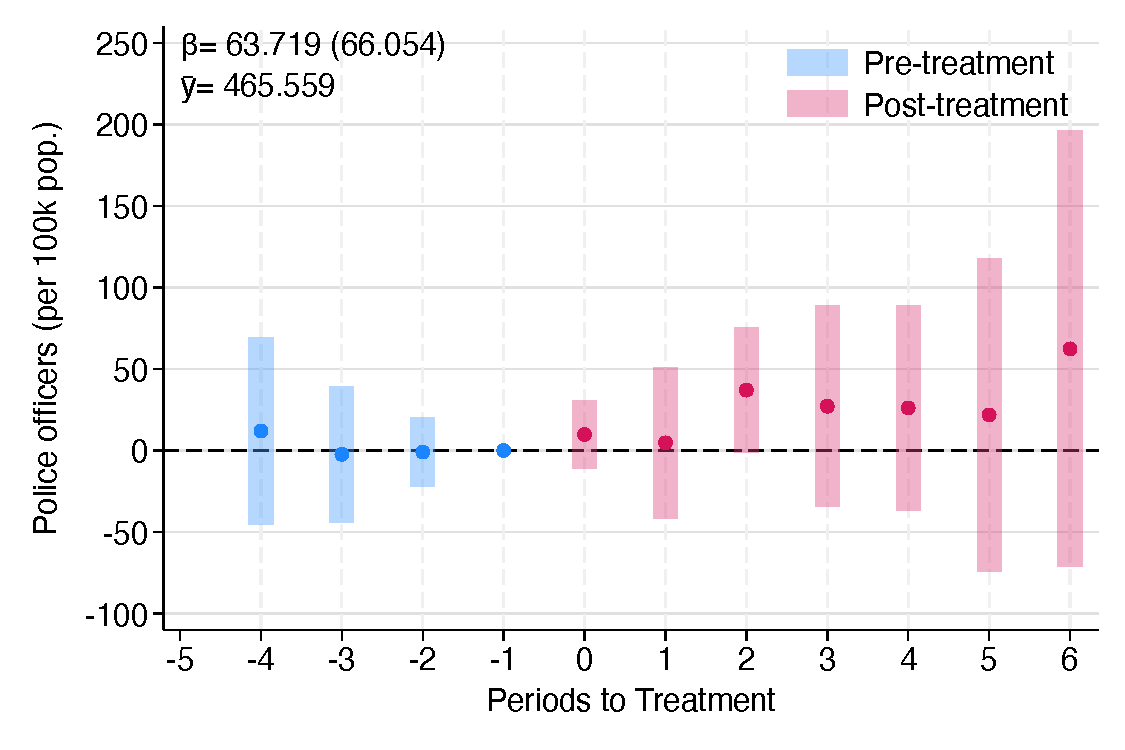
\includegraphics[width=0.98\textwidth]{../manuscript/Graphs/CHDH_continuous_spillover_dotpc.pdf}
        \caption{Spillovers on Police Officers}
    \end{subfigure}%
    ~
    \begin{subfigure}{0.495\textwidth}
        \centering
        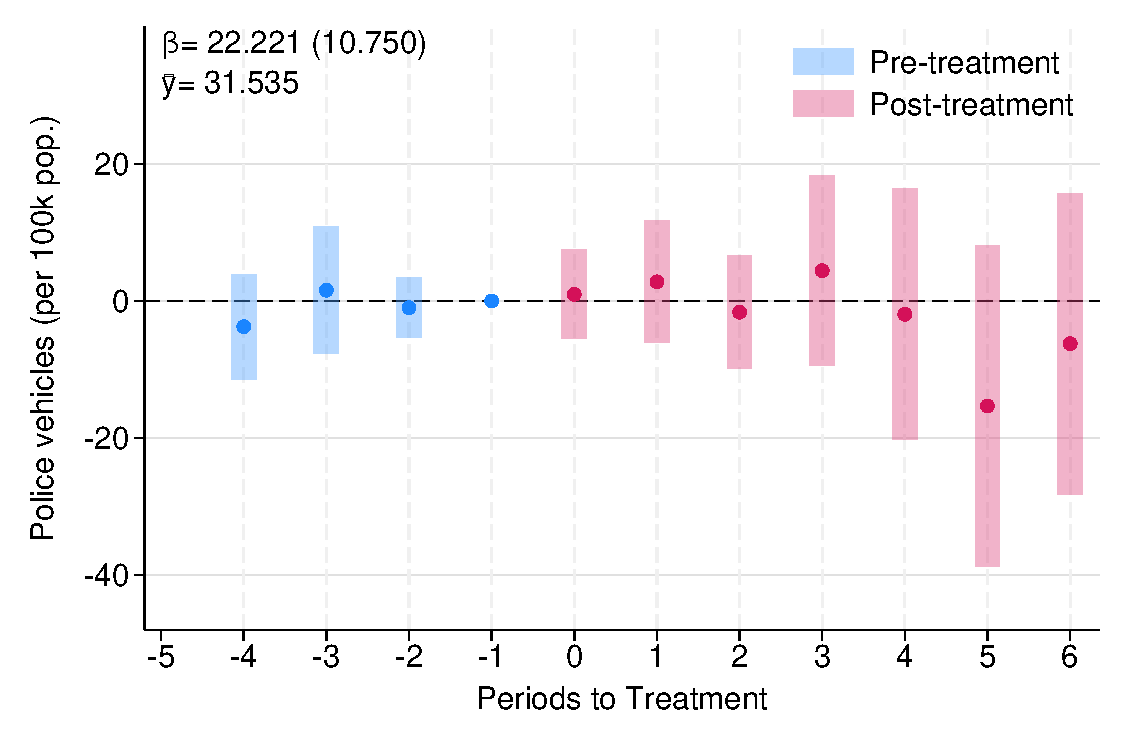
\includegraphics[width=0.98\textwidth]{../manuscript/Graphs/CHDH_continuous_spillover_vehiclespc.pdf}
        \caption{Spillovers on Patrol Vehicles}
    \end{subfigure}

    \begin{minipage}{0.95\textwidth}
    \footnotesize
    Notes: This figure reports the geographic spillover effects of \emph{Plan Cuadrante} on four outcomes for never-treated municipalities: reported crime per 100,000 inhabitants (panel a), arrests per 100,000 inhabitants (panel b), the number of police officers per 100,000 inhabitants (panel c), and the number of patrol vehicles per 100,000 inhabitants (panel d). Unlike the dummy spillover specification, the treatment variable is now continuous and equals the share of neighboring municipalities that have implemented \emph{Plan Cuadrante} by year $t$, following the spillover-intensity approach of \citet{crepon2013}. The sample is restricted to municipalities that never adopted \emph{Plan Cuadrante}. Estimation is performed using the heterogeneity-robust estimator of \citet{Chaisemartin}, which accommodates a continuous, time-varying treatment intensity in a staggered design. The dots represent the estimated dynamic effects and the bars behind them denote 95\% confidence intervals. Standard errors are clustered at the municipality level. The pooled effect  and the mean of the outcome among municipalities with no treated neighbors are reported in each panel.
    \end{minipage}
\end{figure}


\begin{figure}[h!]
    \centering
    \caption{Geographic Spillovers of \emph{Plan Cuadrante} by Number of Treated Neighbors}
    \label{fig:figure_count_spillovers}
    \begin{subfigure}{0.495\textwidth}
        \centering
        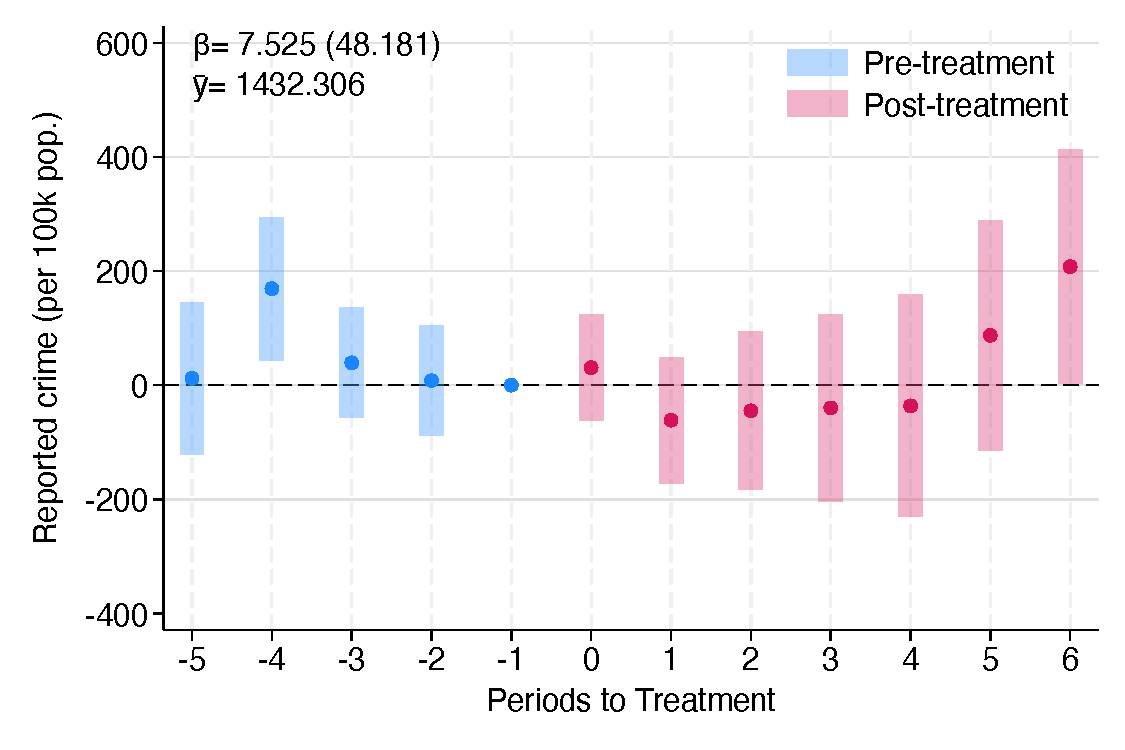
\includegraphics[width=0.98\textwidth]{../manuscript/Graphs/CHDH_continuous_spillover_crime_count.pdf}
        \caption{Spillovers on Reported Crime}
    \end{subfigure}%
    ~
    \begin{subfigure}{0.495\textwidth}
        \centering
        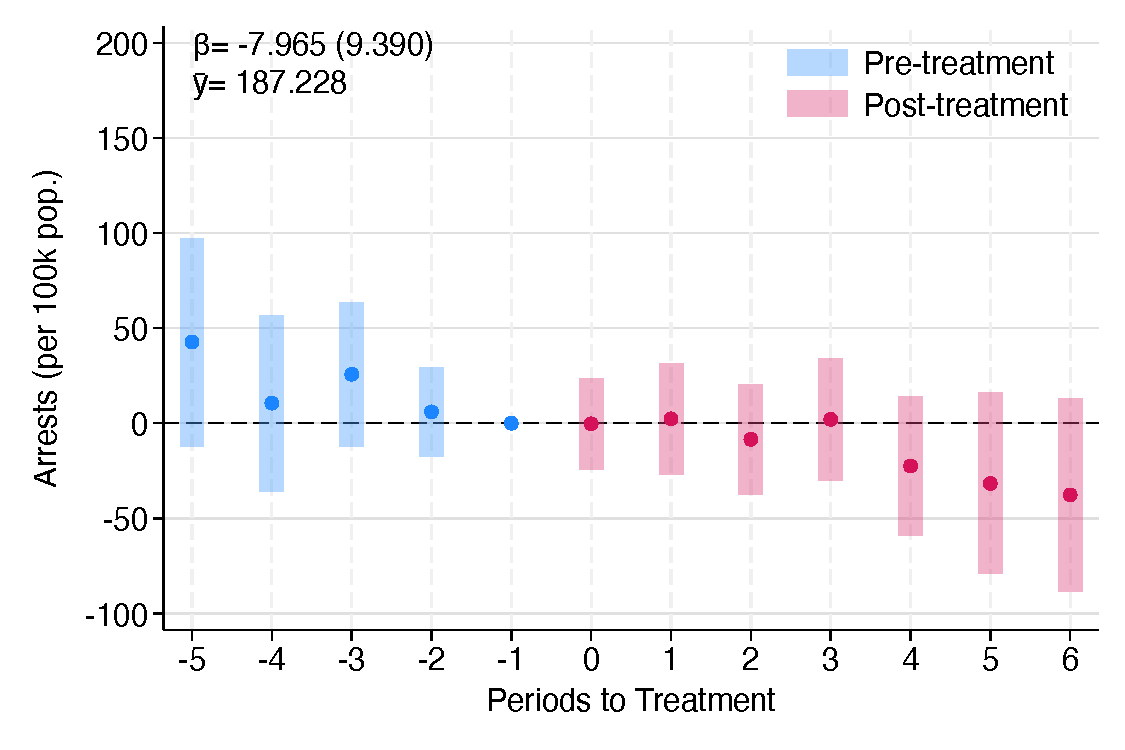
\includegraphics[width=0.98\textwidth]{../manuscript/Graphs/CHDH_continuous_spillover_arrests_count.pdf}
        \caption{Spillovers on Arrests}
    \end{subfigure}

    \vspace{0.5em}

    \begin{subfigure}{0.495\textwidth}
        \centering
        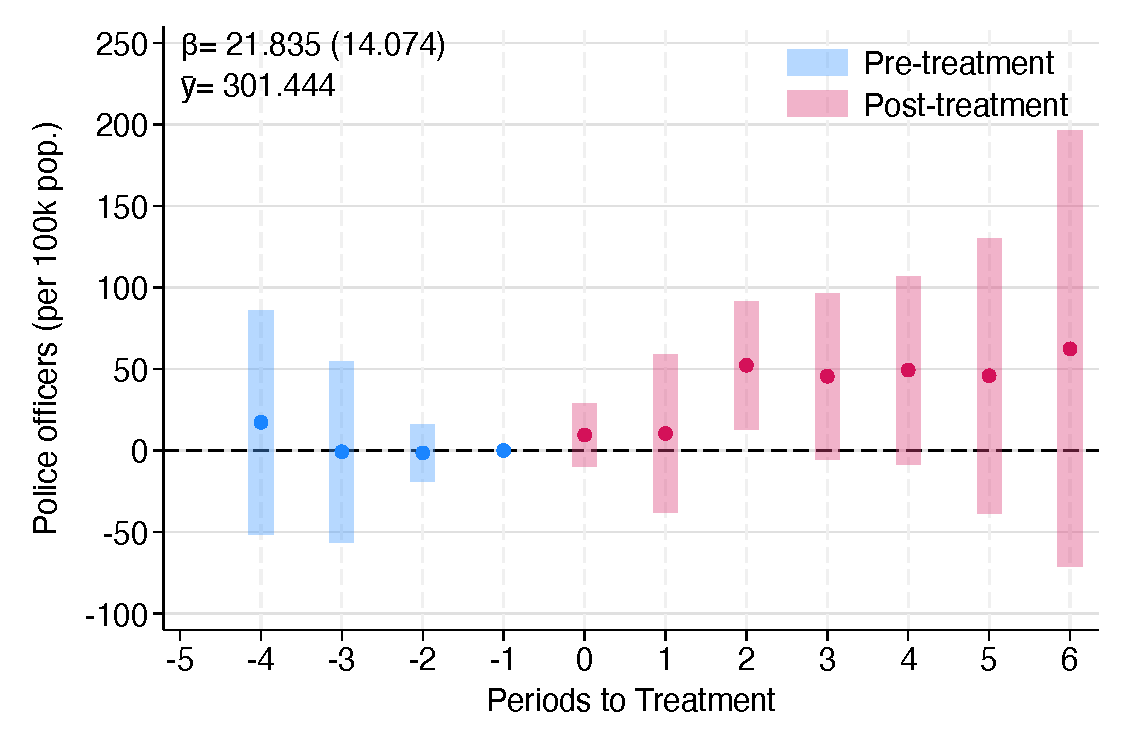
\includegraphics[width=0.98\textwidth]{../manuscript/Graphs/CHDH_continuous_spillover_dotpc_count.pdf}
        \caption{Spillovers on Police Officers}
    \end{subfigure}%
    ~
    \begin{subfigure}{0.495\textwidth}
        \centering
        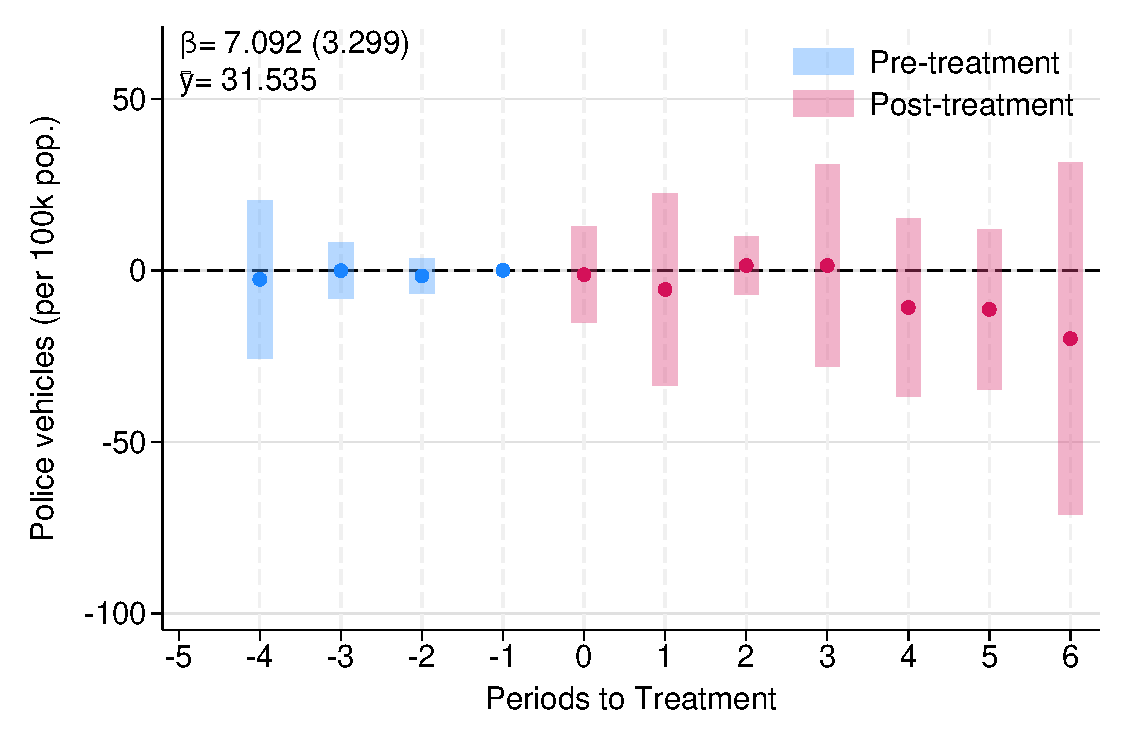
\includegraphics[width=0.98\textwidth]{../manuscript/Graphs/CHDH_continuous_spillover_vehiclespc_count.pdf}
        \caption{Spillovers on Patrol Vehicles}
    \end{subfigure}

    \begin{minipage}{0.95\textwidth}
    \footnotesize
    Notes: This figure reports the geographic spillover effects of \emph{Plan Cuadrante} on four outcomes for never-treated municipalities: reported crime per 100,000 inhabitants (panel a), arrests per 100,000 inhabitants (panel b), the number of police officers per 100,000 inhabitants (panel c), and the number of patrol vehicles per 100,000 inhabitants (panel d). Unlike the dummy spillover specification, the treatment variable is now continuous and equals the number of neighboring municipalities that have implemented \emph{Plan Cuadrante} by year $t$, following the spillover-intensity approach of \citet{crepon2013}. The sample is restricted to municipalities that never adopted \emph{Plan Cuadrante}. Estimation is performed using the heterogeneity-robust estimator of \citet{Chaisemartin}, which accommodates a continuous, time-varying treatment intensity in a staggered design. The dots represent the estimated dynamic effects and the bars behind them denote 95\% confidence intervals. Standard errors are clustered at the municipality level. The pooled effect  and the mean of the outcome among municipalities with no treated neighbors are reported in each panel.
    \end{minipage}
\end{figure}
}

\clearpage

{\renewcommand{\thefigure}{C.15}
\begin{figure}[h!]
    \centering
    \caption{Randomization Inference for the Direct and Spillover Effects of \emph{Plan Cuadrante}}
    \label{fig:ri_placebo}
    \begin{subfigure}{0.495\textwidth}
        \centering
        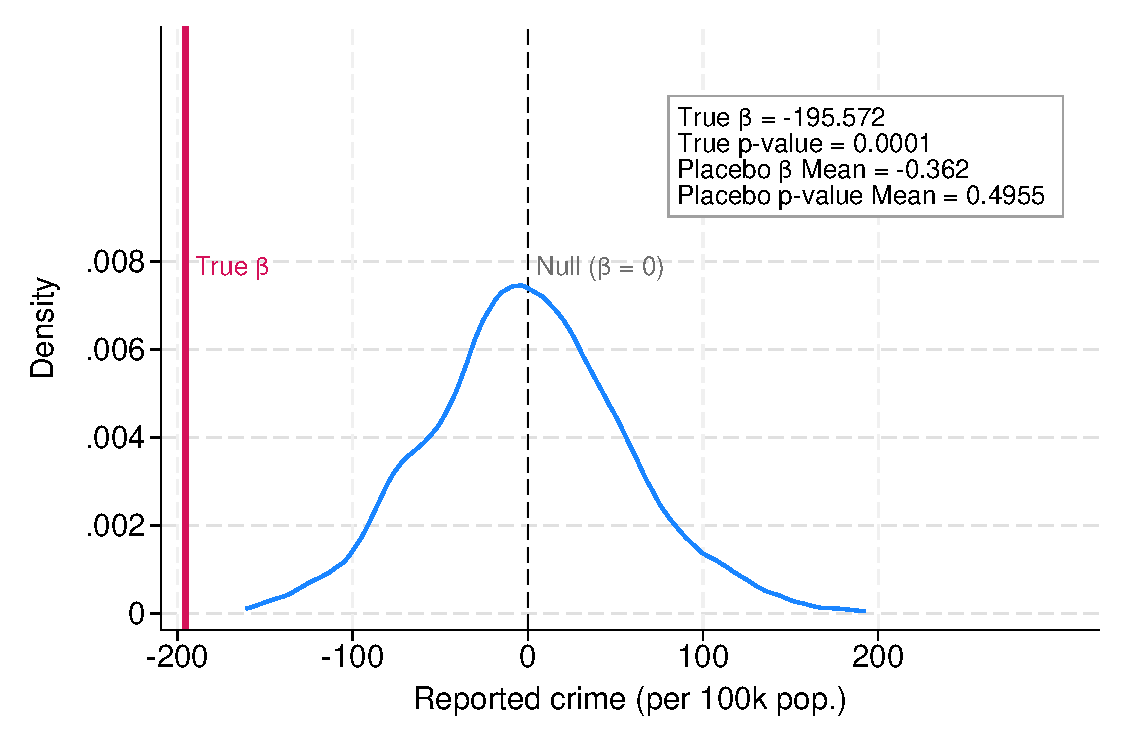
\includegraphics[width=\textwidth]{../manuscript/Graphs/CHDH_RI_placebo_crime.pdf}
        \caption{Reported crime}
        \label{fig:ri_crime}
    \end{subfigure}%
    ~
    \begin{subfigure}{0.495\textwidth}
        \centering
        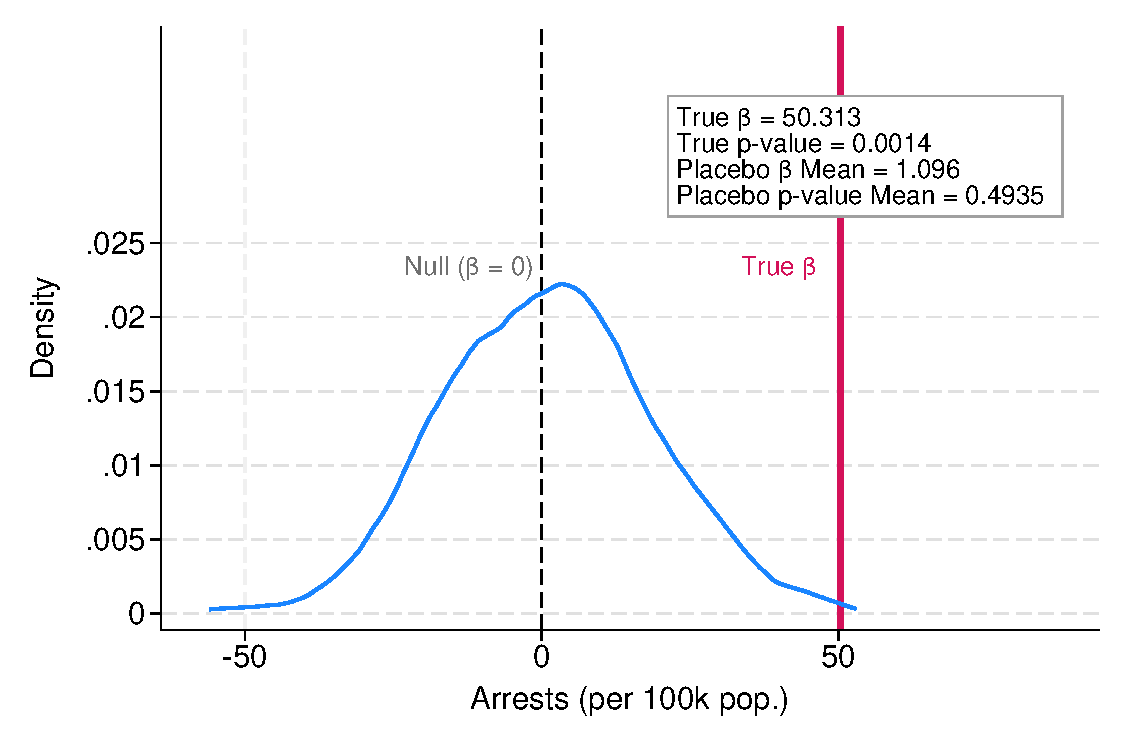
\includegraphics[width=\textwidth]{../manuscript/Graphs/CHDH_RI_placebo_arrests.pdf}
        \caption{Arrests}
        \label{fig:ri_arrests}
    \end{subfigure}

    \begin{subfigure}{0.495\textwidth}
        \centering
        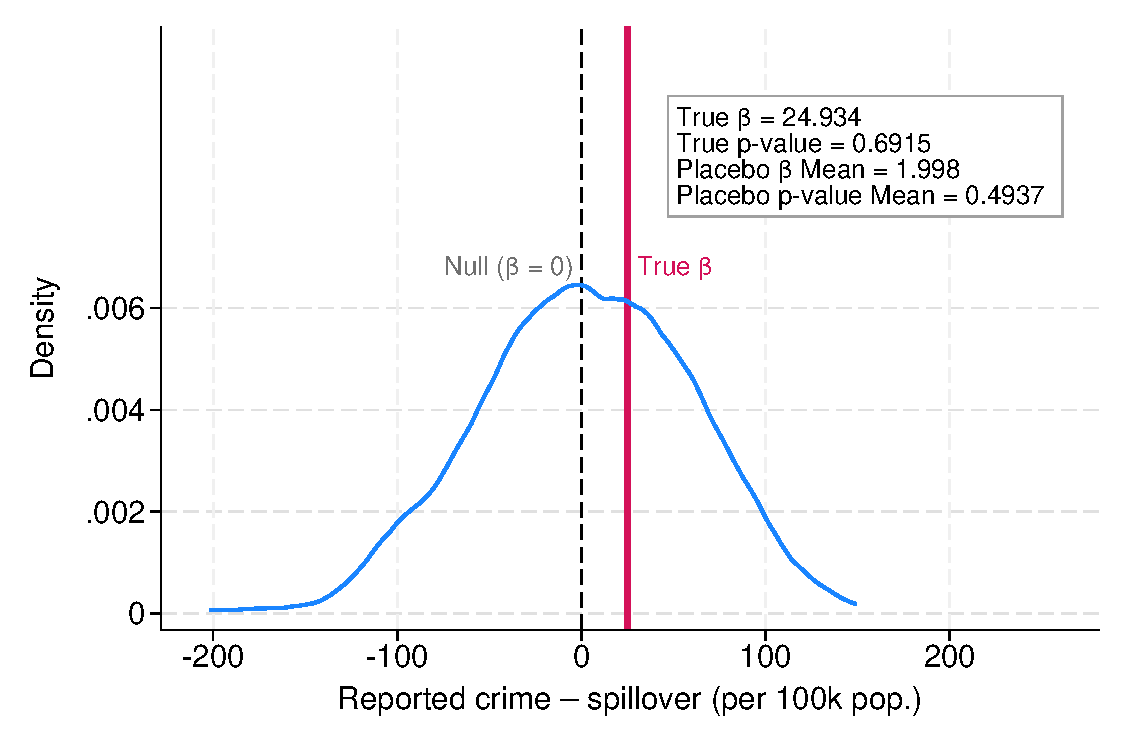
\includegraphics[width=\textwidth]{../manuscript/Graphs/CHDH_RI_placebo_crime_spillover.pdf}
        \caption{Spillovers on Reported crime}
        \label{fig:ri_crime_spillover}
    \end{subfigure}%
    \begin{subfigure}{0.495\textwidth}
        \centering
        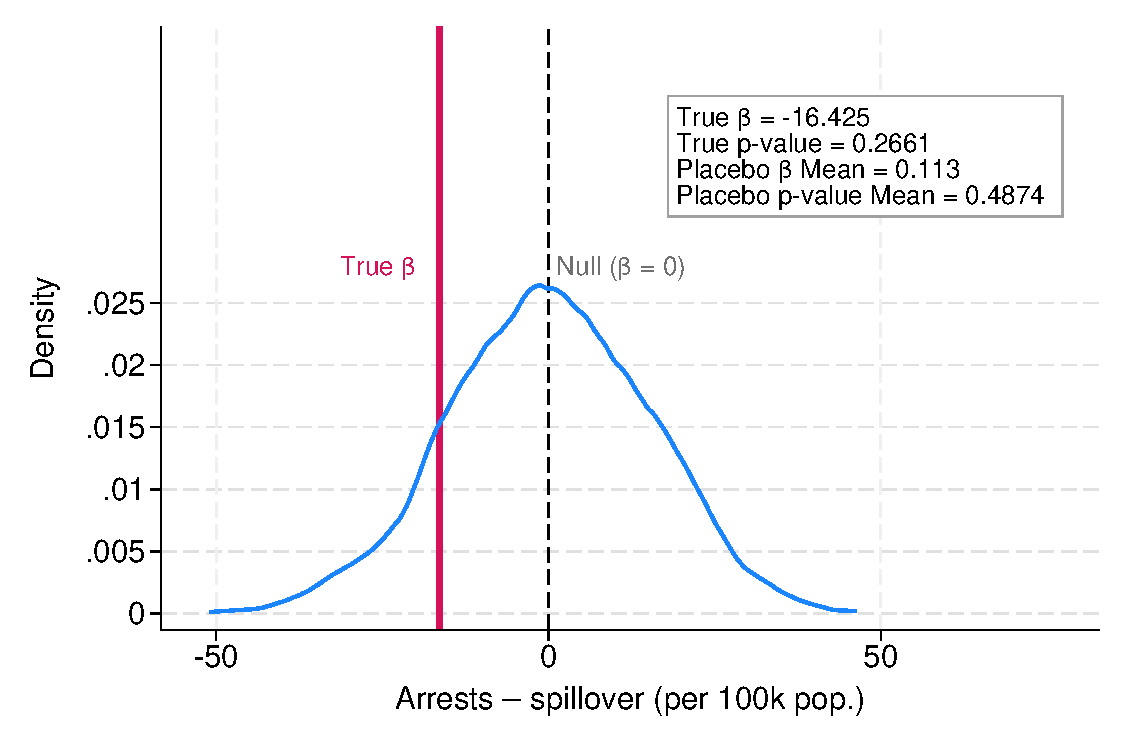
\includegraphics[width=\textwidth]{../manuscript/Graphs/CHDH_RI_placebo_arrests_spillover.pdf}
        \caption{Spillovers on Arrests}
        \label{fig:ri_arrests_spillover}
    \end{subfigure}
    \begin{minipage}{0.95\textwidth}
    \footnotesize
    Notes: This figure presents randomization inference results under the sharp null of no treatment effect, using the heterogeneity-robust estimator of \citet{Chaisemartin}. Each curve is the kernel density of 1{,}000 placebo ATT estimates obtained by jointly permuting \emph{Plan Cuadrante} adoption dates and never-treated status across municipalities (drawing from the empirical distribution of (date, status) pairs, so the marginal counts of treated and never-treated municipalities are preserved in every permutation). In each permutation the variable PC is shuffled across all 346 municipalities and a new time-varying treatment indicator is computed before re-estimating the dynamic effects. The solid colored vertical line marks the point estimate from the true rollout; the dashed black line marks the null expectation $\beta = 0$. The boxes report the true point estimate, its asymptotic two-sided $p$-value, and the mean of the placebo $\beta$ and placebo $p$-value distributions.
    \end{minipage}
\end{figure}
}

\clearpage

{\setcounter{figure}{15}\renewcommand{\thefigure}{C.\arabic{figure}}
\begin{figure}[h!]
    \centering
    \caption{Geographic Spillovers of \emph{Plan Cuadrante} for Neighbors of the ENUSC Municipalities (Administrative Outcomes)}
    \label{fig:figure_46ENUSC_spillovers_admin}
    \begin{subfigure}{0.495\textwidth}
        \centering
        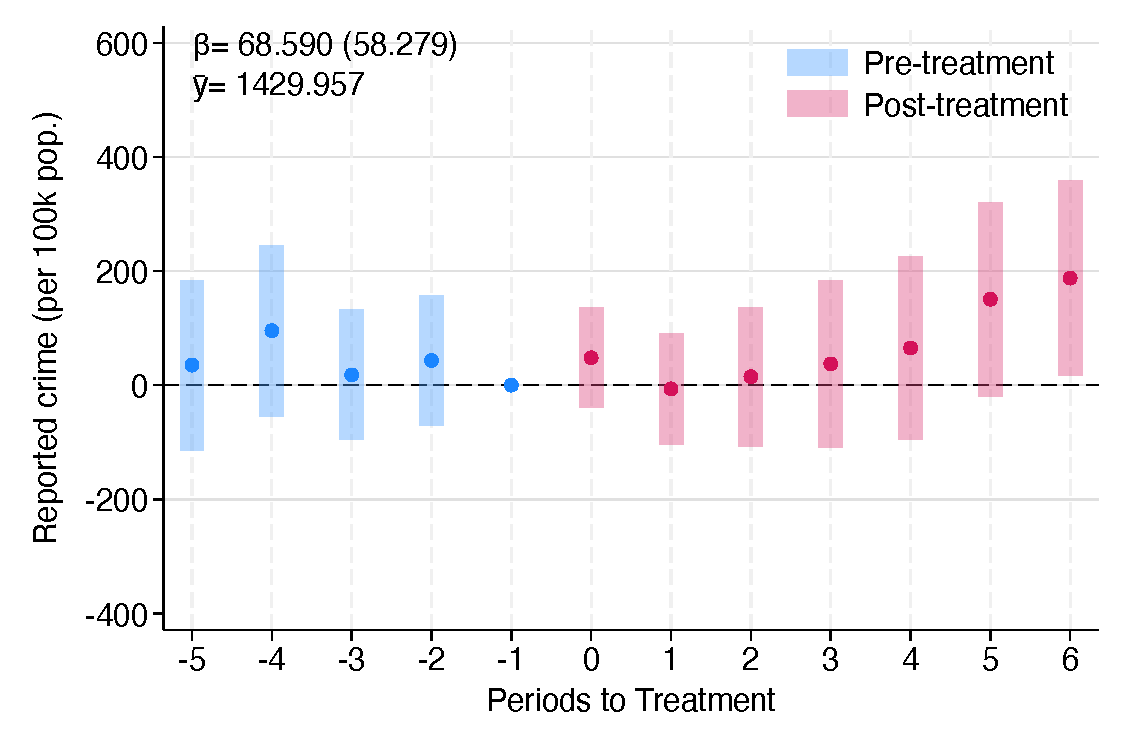
\includegraphics[width=0.98\textwidth]{../manuscript/Graphs/totalreportedcrime_enusc47_neighbors.pdf}
        \caption{Spillovers on Reported Crime}
    \end{subfigure}%
    ~
    \begin{subfigure}{0.495\textwidth}
        \centering
        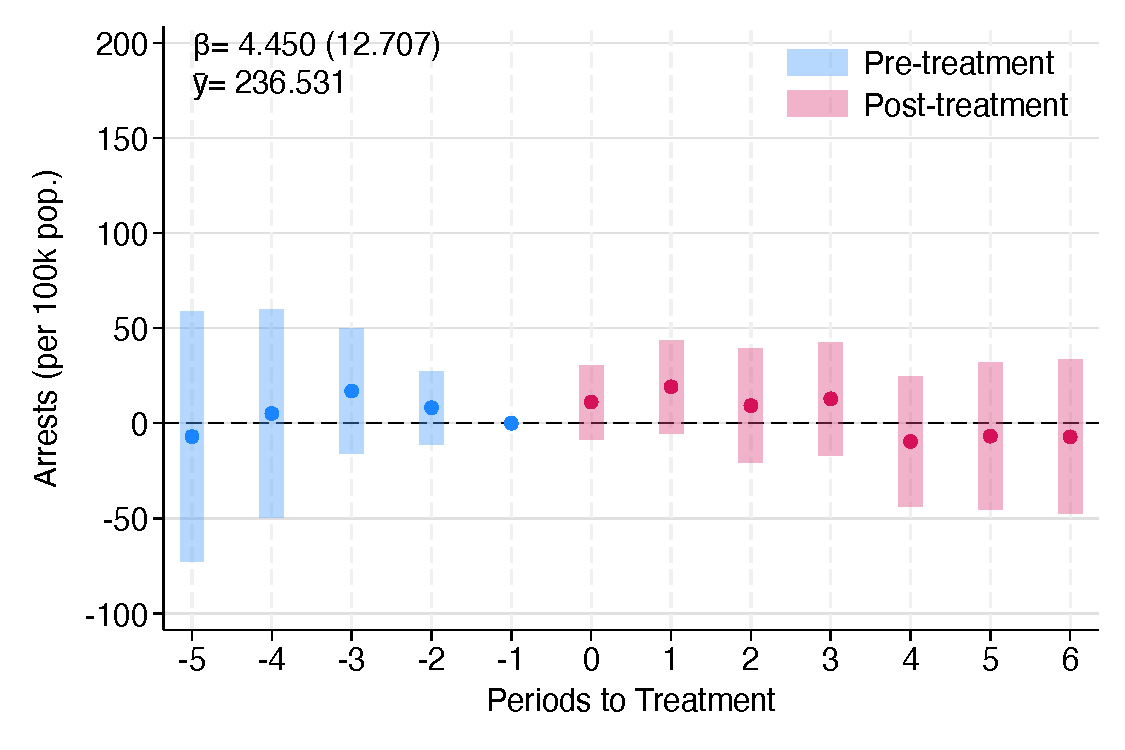
\includegraphics[width=0.98\textwidth]{../manuscript/Graphs/totalarrestscrime_enusc47_neighbors.pdf}
        \caption{Spillovers on Arrests}
    \end{subfigure}

    \vspace{0.5em}

    \begin{subfigure}{0.495\textwidth}
        \centering
        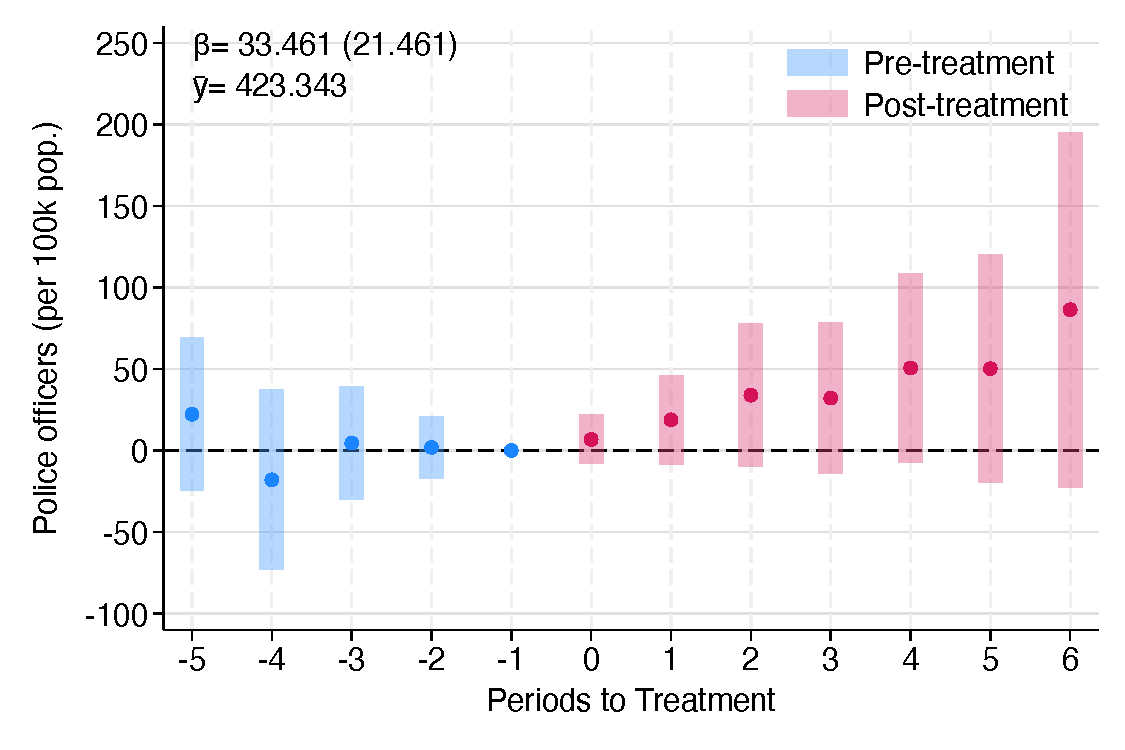
\includegraphics[width=0.98\textwidth]{../manuscript/Graphs/dotpc_enusc47_neighbors.pdf}
        \caption{Spillovers on Police Officers}
    \end{subfigure}%
    ~
    \begin{subfigure}{0.495\textwidth}
        \centering
        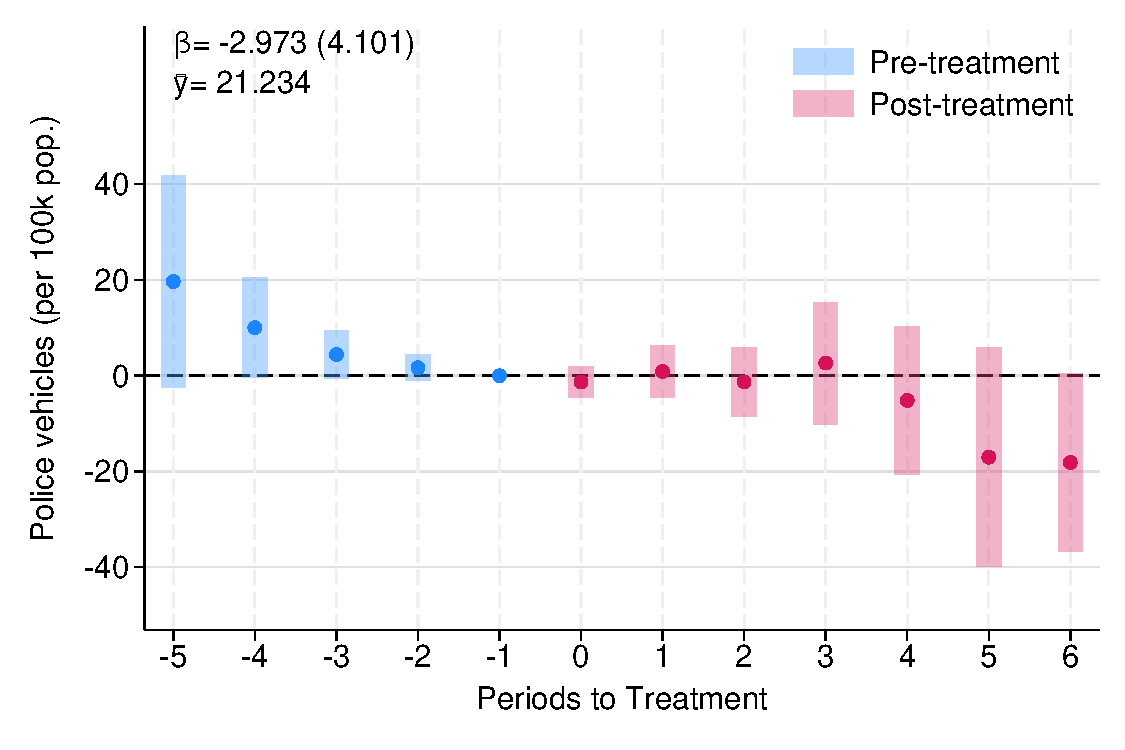
\includegraphics[width=0.98\textwidth]{../manuscript/Graphs/vehiclespc_enusc47_neighbors.pdf}
        \caption{Spillovers on Patrol Vehicles}
    \end{subfigure}

\begin{minipage}{\textwidth}
\footnotesize Notes: This figure reports the spillover effects of \emph{Plan Cuadrante} on the number of crimes reported to the police in the municipality per 100,000 inhabitants (panel a), on the number of arrests in the municipality per 100,000 inhabitants (panel b), on the number of police officers (panel c), and on the number of patrol vehicles (panel d). Specifically, the figure shows the dynamic effects of \emph{Plan Cuadrante} for neighboring never-treated municipalities to the 46 municipalities included in the ENUSC sample. The estimation is conducted using the procedure developed in \citet{Callaway} for difference-in-differences with staggered treatment adoption, using as the treatment introduction date the earliest date of a neighboring municipality. The dots in the figure represent the estimated coefficients and the bars behind them 95\% confidence intervals. Standard errors are clustered at the municipality level using the wild bootstrap procedure. The pooled effect and the mean outcome before the introduction of the treatment for each outcome are also presented in each panel.
\end{minipage}
\end{figure}


\begin{figure}[h!]
    \centering
    \caption{Geographic Spillovers of \emph{Plan Cuadrante} on ENUSC Survey Outcomes (Early- to Late-Adopting Municipalities)}
    \label{fig:figure_results_spillovers_enusc}
    \begin{subfigure}{0.495\textwidth}
        \centering
        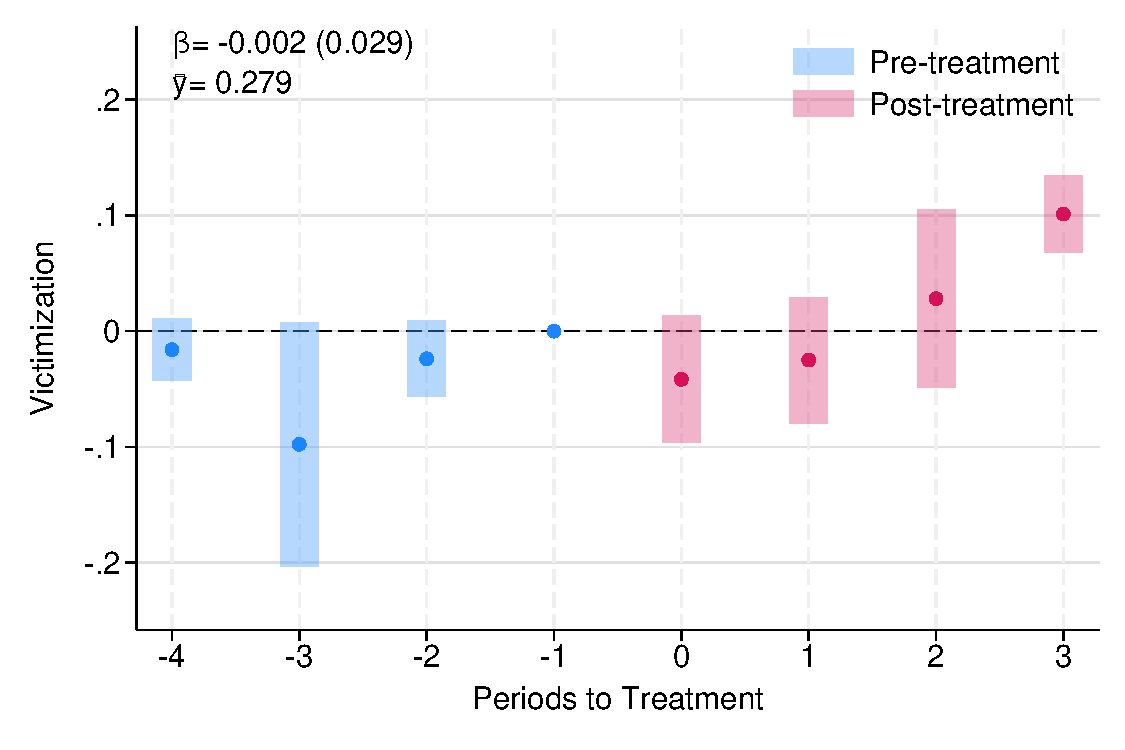
\includegraphics[width=0.98\textwidth]{../manuscript/Graphs/results_spillover_delitos.pdf}
        \caption{Spillovers on Victimization in last 12 months}
    \end{subfigure}%
    ~
    \begin{subfigure}{0.495\textwidth}
        \centering
        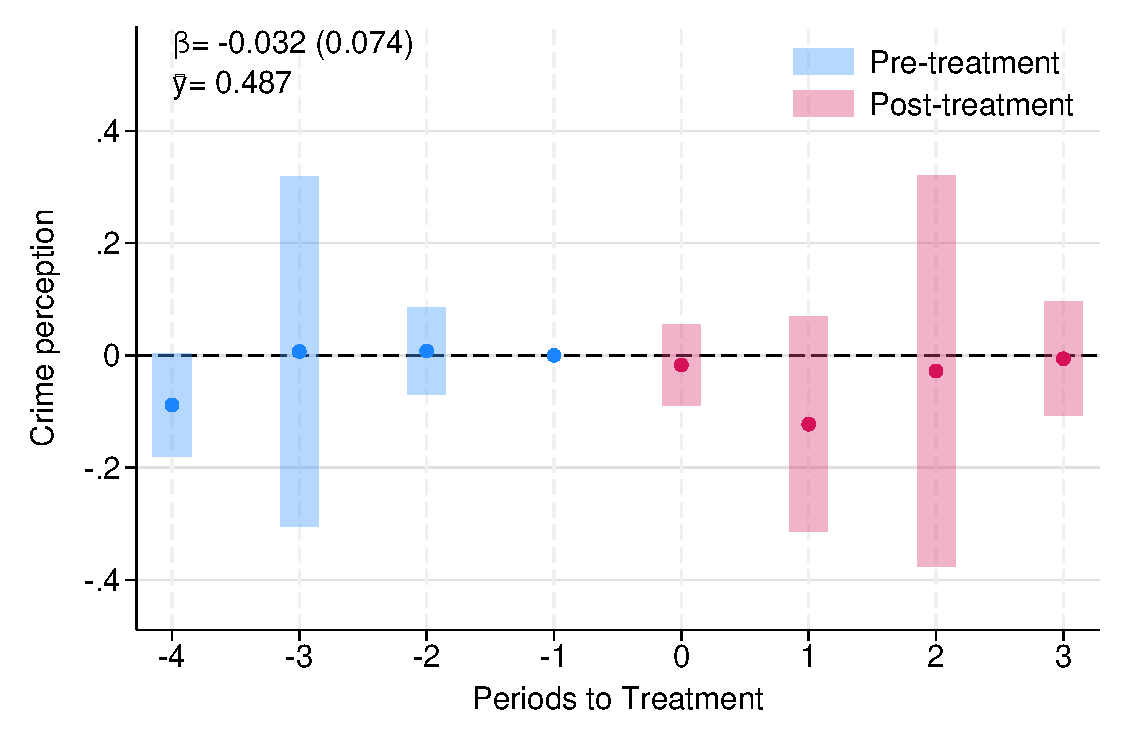
\includegraphics[width=0.98\textwidth]{../manuscript/Graphs/results_spillover_inseguridad_barrio1.pdf}
        \caption{Spillovers on Households reporting an increase in crime}
    \end{subfigure}
    \vspace{0.5em}
    \begin{subfigure}{0.495\textwidth}
        \centering
        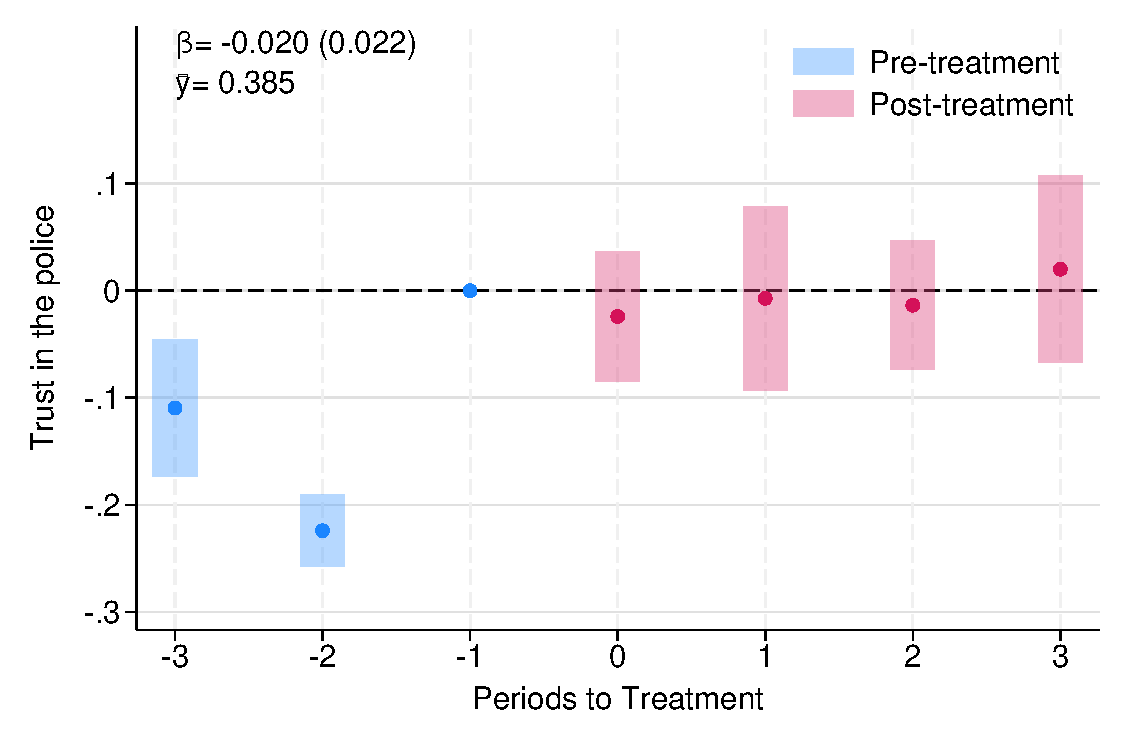
\includegraphics[width=0.98\textwidth]{../manuscript/Graphs/results_spillover_confianza_carabineros.pdf}
        \caption{Spillovers on Trust in the police}
    \end{subfigure}%
    ~
    \begin{subfigure}{0.495\textwidth}
        \centering
        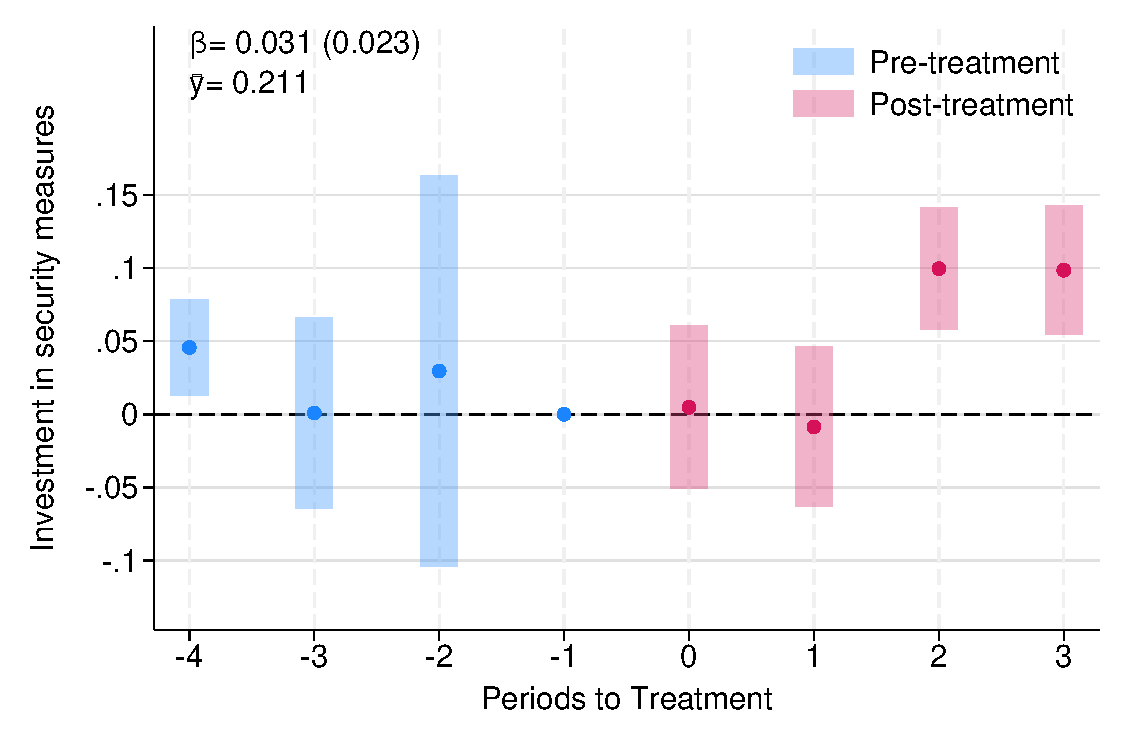
\includegraphics[width=0.98\textwidth]{../manuscript/Graphs/results_spillover_medidas_general_12.pdf}
        \caption{Spillovers on Households adopting security measures}
    \end{subfigure}
    \begin{minipage}{0.95\textwidth}
    \footnotesize
    Notes: This figure presents the geographic spillover effects of \emph{Plan Cuadrante} from early-adopting ENUSC municipalities on their late-adopting ENUSC neighbours, using the ENUSC sample. Panel (a) reports the effect of \emph{Plan Cuadrante} on the probability of household victimization in the last 12-months using the ENUSC survey. Panel (b) reports the effect on crime perception using the ENUSC survey. Panel (c) reports the effect on trust in the police using the ENUSC survey. Panel (d) reports the results on the probability of purchasing private security measures in the last twelve months using the ENUSC survey. The focal treated sample consists of six late-adopting ENUSC municipalities---Molina, Tocopilla, San Carlos, Padre Hurtado, Calera, and Limache---each assigned a spillover-onset date equal to the year its earliest-adopting ENUSC neighbour received \emph{Plan Cuadrante}: Curic\'o (2005) for Molina, Iquique (2005) for Tocopilla, Chill\'an (2007) for San Carlos, Pe\~naflor (2008) for Padre Hurtado, and Quillota (2008) for both Calera and Limache. Estimation is performed using the difference-in-differences estimator for staggered treatment adoption of \citet{Callaway}. The dots represent the estimated dynamic effects and the bars behind them denote 95\% confidence intervals. Standard errors are clustered at the municipality level. The pooled effect  and the mean of the outcome among municipalities with no treated neighbors are reported in each panel.
    \end{minipage}
\end{figure}

}

\clearpage


\end{response}
\stepcounter{AnsweredComments}




% Comment R2 - 4
\begin{refcomment}

\smallskip

Relatedly, criminals may easily cross municipal boundaries in Chile. Can you report the share of offenders apprehended in municipality X who committed crimes elsewhere? How should the reader think about this?

\label{pt:r2_04}
\end{refcomment}

\begin{response}
    %I also noticed that some estimates based on the administrative data have changed between the two versions. In particular, the estimated reduction in reported crime is now 10 percent rather than 14 percent. I could not find this change documented in the response. As long as the authors can provide a reasonable explanation for what changed between rounds and are confident that the current result is robust, I do not view this as a major concern.


Thanks for pointing this out, and apologies for not documenting this change explicitly in our previous response.

The change in the headline number---from a 14\% to a 10\% decline in reported crime--- comes mainly from a change in how we compute $\hat{Y}$, the baseline level we use as the denominator to convert that level effect into a percentage change. In the previous version, $\hat{Y}$ was computed as a simple average over the pooled sample of observations---pre-treatment observations of treated municipalities together with observations from never-treated municipalities---rather than as an average of the two groups' separate means. Since the Callaway and Sant'Anna estimator is essentially a treatment-on-the-treated (ToT) parameter, we now believe it is more appropriate to compute $\hat{Y}$ using only the pre-treatment observations of treated municipalities. This revision affects the administrative-data-based estimates more evidently than the ENUSC-based ones, because the administrative sample includes 196 never-treated municipalities, whereas the ENUSC sample includes only one; pooling into $\hat{Y}$ therefore moved the administrative baseline by much more than the ENUSC one. We apologize again for not flagging this change explicitly in our earlier response. To avoid this ambiguity going forward, we now define $\hat{Y}$ explicitly in the notes of every figure that reports it.

A second, unrelated and more minor change may also explain very minor differences in some $\beta$ coefficients (including the headline estimate). Between the first and second submission we realized that our implementation of the Callaway and Sant'Anna estimator was not weighting estimates by cohort size, while the default ``simple'' and ``dynamic'' aggregation schemes in \citet{Callaway} weight by cohort size (DANI INCLUYE AQUI ALGUNA CITA PORFA -- adicional a Callaway, si tienes una referencia mas especifica sobre el uso de este peso por defecto en la practica, mejor). We corrected this, which slightly changes some point estimates but not in a way that is economically or statistically meaningful.





\end{response}
\stepcounter{AnsweredComments}


% Comment R2 - 5
\begin{refcomment}

Interpretation of the Results: The authors argue that the effects on crime are driven primarily by geographic specialization, rather than additional resources, and leverage variation in the amount of additional resources across municipalities to provide evidence for their claim. However, it is unclear from the paper what drives the variation in additional resources. If municipalities experiencing larger increases in crime are those getting larger increases in resources, then this margin of exposure to the “resource channel” is endogenous. The paper may benefit from explaining what determines the variation in resources across municipalities and whether it correlates with trends in crime. As mentioned above, it may also help to provide more details on “Plan Cuadrante” such as whether it was accompanied by public information campaigns or media coverage, which could plausibly affect perceptions of security (one of their key outcomes) independently of actual crime rates (see Ajzenman et al. 2023 on this mechanism).

\label{pt:r2_05}
\end{refcomment}

\begin{response}
    % Comment 5: Interpretation of the Results: The authors argue that the effects on crime are driven primarily by geographic specialization, rather than additional resources, and leverage variation in the amount of additional resources across municipalities to provide evidence for their claim. However, it is unclear from the paper what drives the variation in additional resources. If municipalities experiencing larger increases in crime are those getting larger increases in resources, then this margin of exposure to the “resource channel” is endogenous. The paper may benefit from explaining what determines the variation in resources across municipalities and whether it correlates with trends in crime. As mentioned above, it may also help to provide more details on “Plan Cuadrante” such as whether it was accompanied by public information campaigns or media coverage, which could plausibly affect perceptions of security (one of their key outcomes) independently of actual crime rates (see Ajzenman et al. 2023 on this mechanism).

Thanks for the comment. Let us start by clarifying our main claim: we do not argue that the additional resources brought by \emph{Plan Cuadrante} have no effect on crime. Our key finding in the heterogeneity analysis by resource increases is that even municipalities that experienced no increase in resources relative to the control group show sizeable effects on nearly every outcome considered (see Figure \ref{fig:figure02}). In this context, where resource increases may be endogenous, we cannot rule out a role for resources in explaining the effects of \emph{Plan Cuadrante} in municipalities that received large increases, nor can we rule out that resources were important for the successful implementation of the beat policing component in those municipalities. However, the finding that municipalities with no additional resources relative to the control group still experience sizeable effects provides clear evidence that the beat policing component of the program plays an important independent role, which is our main point. Consistent with this, and in line with the revised manuscript, we now emphasize that these effects remain sizeable in municipalities with resource increases similar to those in control municipalities. We also find that subsequent increases in police resources outside \emph{Plan Cuadrante} have very limited effects on victimization. First, conditional on municipality and year fixed effects, changes in resources are not associated with reductions in crime. Second, we estimate the effect of a national program that increased police resources without any organizational component and find null effects on crime. Finally, the main estimates are robust to the inclusion of police resources as control variables, which, while by definition bad controls as they are themselves affected by \emph{Plan Cuadrante}, do not meaningfully alter the coefficients.


On what determined the size of the resource increases: During the 2000s and 2010s, the Chilean government substantially increased the overall number of Carabineros and other police resources such as patrol vehicles, and this increase benefited both treated and control municipalities. On top of this general trend, \emph{Plan Cuadrante} aimed to provide treated municipalities with sufficient additional resources to successfully implement the program. Panels (c) and (d) of Figure \ref{fig:figure05} show that, on average, \emph{Plan Cuadrante} substantially increased police resources relative to the control group. Panels (a) and (b) of Figure \ref{fig:figure_resources} show, however, that this increase masks substantial heterogeneity across treated municipalities: while municipalities in the bottom 40\% of the resource-increase distribution experienced increases very similar to those observed in control municipalities, municipalities in the top 40\% experienced substantially larger increases, with officers rising annually by around 22\% and patrol vehicles by around 80\% upon joining \emph{Plan Cuadrante}. So, what drives the variation in additional resources across treated municipalities? In principle, the goal was for \emph{Plan Cuadrante} to increase resources enough to cover each municipality's pre-existing resource deficit, measured in Equivalent Surveillance Units (UVEs). However, program documents make clear that budgetary constraints meant that all municipalities joined \emph{Plan Cuadrante} without fully closing this gap \citep{DIPRES2014, DIPRES2007_largo}, and program evaluations do not clearly establish that the size of this remaining deficit is what determined the resource increase each municipality received. We asked Carabineros for access to the official demand and supply figures that were supposed to guide this allocation, but this information was not provided. Importantly, we find that municipalities receiving larger versus smaller resource increases---whether the split is based on the increase in police officers or in patrol vehicles---do not display differential pre-treatment trends in either the outcomes of interest or in police resources themselves.\footnote{The p-values for the joint test of equal pre-trends between the two groups are, for the officers-based split and the patrol-vehicles-based split respectively: 0.823 and 0.048 for victimization, 0.059 and 0.379 for crime perception, 0.820 and 0.157 for investment in security measures, 0.213 and 0.419 for reported crime, 0.616 and 0.444 for police officers, and 0.405 and 0.157 for patrol vehicles.} We also explore the correlates of the resource increase in Online Appendix B, where we show that pre-treatment outcomes levels are not predictive of the size of the resource increase, while structural municipality characteristics such as population and poverty are more predictive.


Regarding the possibility that the effects on crime perception are driven by accompanying public information campaigns or media coverage, we believe this is unlikely for two reasons. First, \emph{Plan Cuadrante} was an internal operational reform of Carabineros with no formal public communication component in its design. While the program received some media attention when it was broadly rolled out across Santiago in 2000, we find no evidence of targeted information campaigns at the municipality level when individual municipalities subsequently joined the program, and the staggered rollout over more than a decade makes a sustained media salience mechanism implausible. Second, and more importantly, if the improvement in crime perception were driven by media coverage or information campaigns, one would expect the effects to be concentrated shortly after adoption and to fade over time. Instead, the dynamic estimates show that the effects on crime perception grow and persist over time, a pattern more consistent with a genuine improvement in security than with a transitory salience effect of the kind documented in \citet{Ajzenman_Pato}.

All these implementation details are provided in Section 2 in the updated manuscript, which expands substantially the section describing the implementation of \emph{Plan Cuadrante}:

\begin{adjustwidth}{2em}{0em}
{\setcounter{figure}{0}\renewcommand{\thefigure}{\arabic{figure}}
Carabineros, Chile's national police force, was founded in 1927. Through most of our study period, Carabineros operated under the Ministry of Defense, which oversaw both military and police functions until domestic security responsibilities were transferred to the Ministry of Interior in 2011.\footnote{Currently, Carabineros reports to the Ministry of Public Security, created in 2024 to focus exclusively on domestic security.}

Carabineros' mission, functions, and structure are established by Law 18.961 and the Regulation on Carabineros' Organization (Reglamento de Carabineros) \citep{Ley18961,ReglamentoCarabineros1989}. Under this framework, Carabineros is a professional, disciplined, and hierarchical police institution whose mission is to preserve public order and security with a central emphasis on preventive policing. The General Director heads the strategic level, responsible for defining doctrine and institutional strategy, while the Subdirector coordinates implementation. The Directorate of Order and Security administers police functions at the tactical level.

Territorially, Carabineros is organized into zones that oversee \emph{prefecturas}. Zones and \emph{prefecturas} are primarily management layers. Zones map roughly one-to-one to Chile's regional divisions, with two exceptions: the Metropolitan Region of Santiago---the most populated in the country---and La Araucanía---which has recently experienced significant social conflict---are each divided into two zones. Each zone is subdivided into \emph{prefecturas}---54 nationwide---which supervise 227 \emph{comisar\'ias}, the main operational units at the tactical level. These \emph{comisar\'ias} oversee smaller units---\emph{subcomisar\'ias}, \emph{tenencias}, \emph{retenes}, \emph{puestos}, and \emph{avanzadas}---that operate within their assigned jurisdictions.\todo{JORGE: Since we need to cut on the manuscript, I believe this paragraph is a good candidate to be removed or shortened.}

In practice, the \emph{comisar\'ia} is the basic unit of routine frontline policing and, in most municipalities, serves as the territorial anchor of police work. Officers conduct patrol, surveillance, prevention, and first response at this level. In most municipalities, a single \emph{comisar\'ia} covers the entire municipal territory, though larger municipalities may have multiple ones. Santiago, for instance, has four. %By contrast, 112 municipalities---mostly remote or rural---have no \emph{comisar\'ia} and are served through smaller subordinate posts linked to a \emph{comisar\'ia}. 
All municipalities that adopted \emph{Plan Cuadrante} during our study period had a \emph{comisar\'ia}. With the exception of 9 municipalities, each had a single \emph{comisar\'ia} covering the full municipal territory. On average, a \emph{comisar\'ia} in our sample covered 1,608 square kilometers and served 57,642 inhabitants. %Of these, 17 had no subordinate units, whereas the remaining 79 had between one and nine.

\emph{Plan Cuadrante} was introduced within this institutional framework without altering Carabineros' hierarchical structure or its strategic and tactical levels. The reform emerged in a context of rising victimization and insecurity, with the explicit goal of reversing these trends \citep{PCSP2014}. Its central innovation was a shift toward a beat policing model. In the criminology literature, beat policing refers to assigning officers to fixed territorial areas so they can accumulate local knowledge, strengthen ties with residents, and respond more effectively to local crime patterns \citep{cordner1995community,skogan1997comminuty}. In practice, the catchment area of police forces in municipalities adopting \emph{Plan Cuadrante} was partitioned into smaller, fixed geographic units (quadrants), to which officers were permanently assigned. Rather than building new infrastructure, the reform redefined the territorial responsibility of officers in already existing police stations \citep{DIPRES2007_largo}.\footnote{In 2016, Carabineros launched the \emph{Plan Cuadrante 2.0} program in those municipalities served by \emph{Plan Cuadrante}. While this reform introduced additional reforms aimed at integrating the community into the provision of security and building capacity to gather and analyze crime data in police stations, this paper's study period ends before these improvements were introduced.} This represented a clear break from the pre-reform system, in which officers rotated across broad operational territories, very often spanning entire municipalities.

Carabineros began piloting \emph{Plan Cuadrante} in 1998. The program expanded gradually through 2013, as shown in Panel (a) of Figure \ref{fig:figure01}, reaching 150 urban municipalities and covering roughly 90\% of Chile's population.\footnote{Further details about the expansion of \emph{Plan Cuadrante} are provided in Online Appendix \ref{sec:appendixA} and Table \ref{tab:implementation}.} Online Appendix A provides further details about the rollout of the program. The rollout was designed to follow a municipality ranking based on a weighted index of victimization, police resource deficits, drug prevalence, unemployment, and demand for police services, with annual entry determined by available budget.\footnote{The weights assigned to each component changed on a yearly basis \citep{DIPRES2007_largo,DIPRES2014}.} In practice, however, Budget Office evaluations show that adoption diverged from this ranking for undocumented reasons, so the rule operated more as a loose guideline than as a binding assignment mechanism \citep{DIPRES2014}.

\FloatBarrier
%--- Implementation
\begin{figure}[h!]
    \centering
    \caption{Implementation of \emph{Plan Cuadrante}}
    \label{fig:figure01}
    \begin{subfigure}{0.58\textwidth}
        \centering
        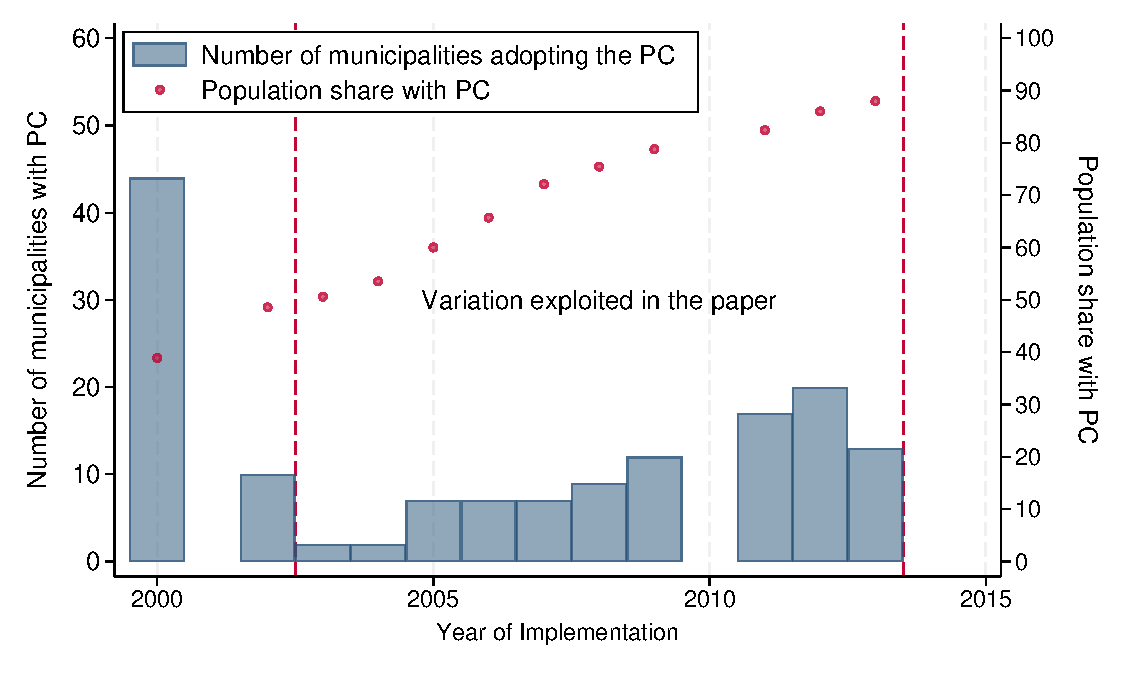
\includegraphics[width=1\textwidth]{../manuscript/Graphs/Graph_PCvariation.pdf}
        \caption{Adoption of \emph{Plan Cuadrante}}
    \end{subfigure}
    \\
    \begin{subfigure}{\textwidth}
    \centering
    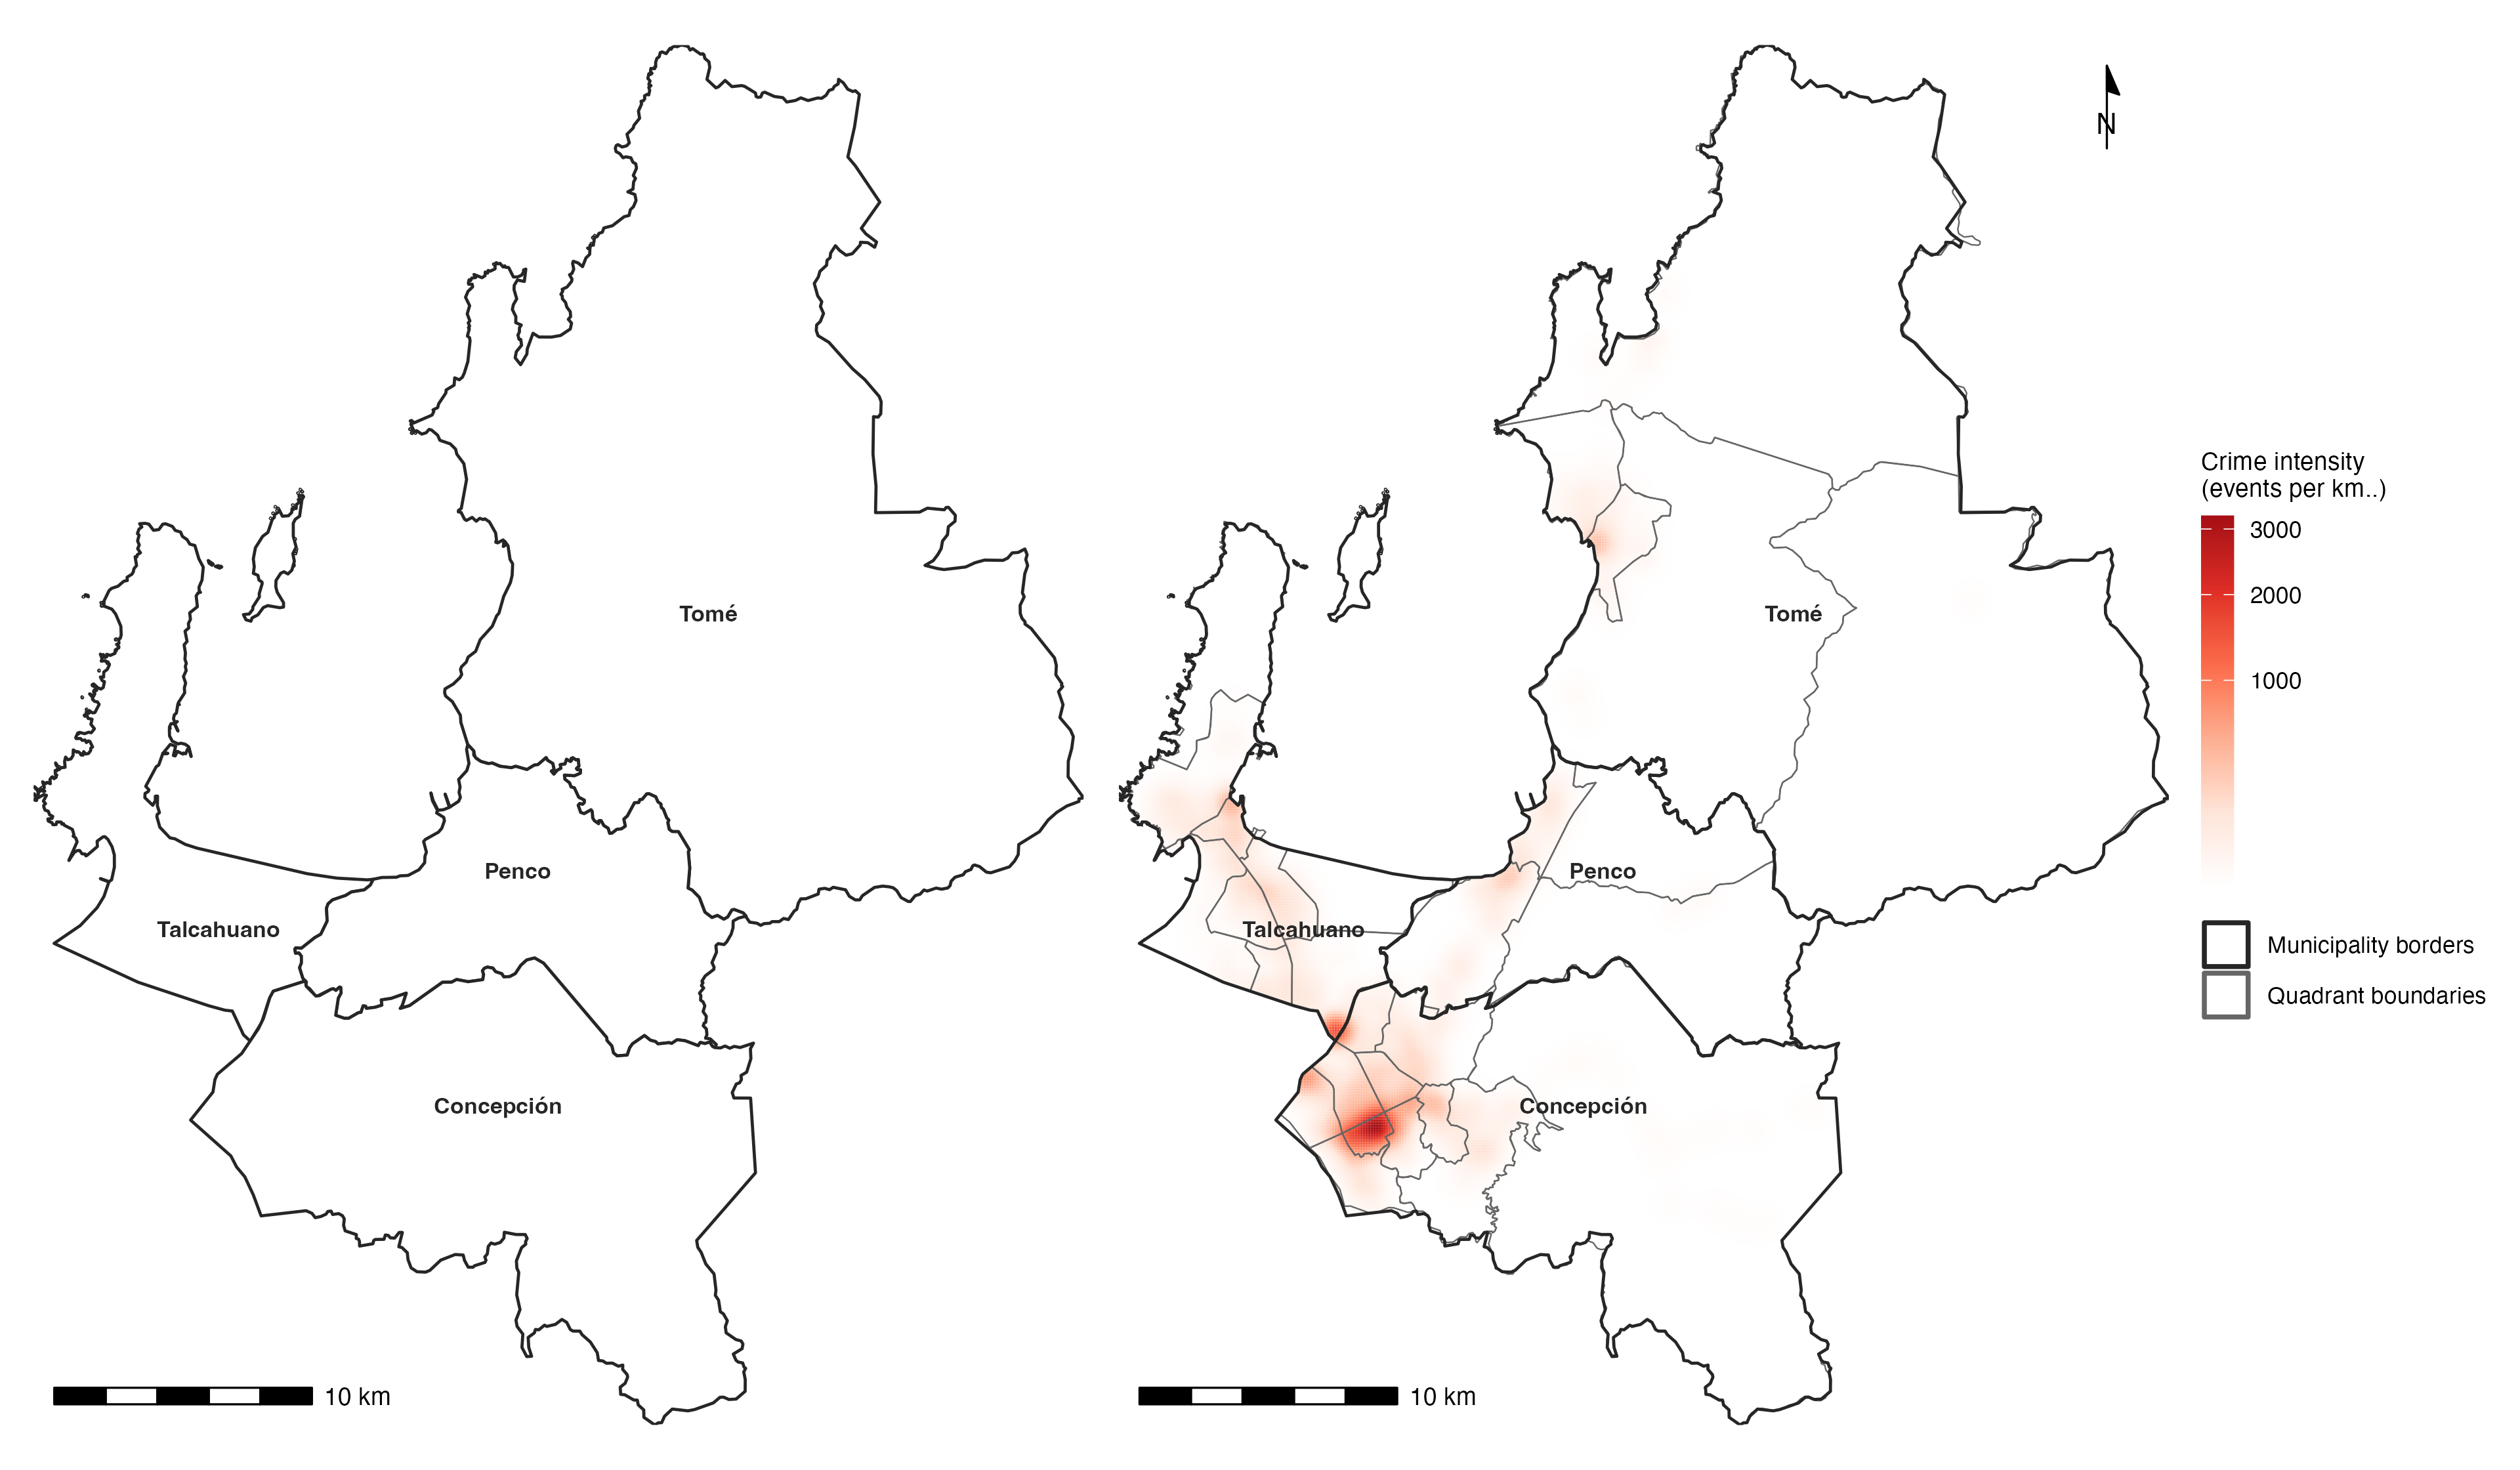
\includegraphics[width=0.65\linewidth]{../manuscript/Graphs/Graph_PCexample_combined.png}
    \caption{\emph{Plan Cuadrante} in the Concepci\'on area}
    \end{subfigure}%
 %   \\
 %   \begin{subfigure}{0.58\textwidth}
 %       \centering
 %       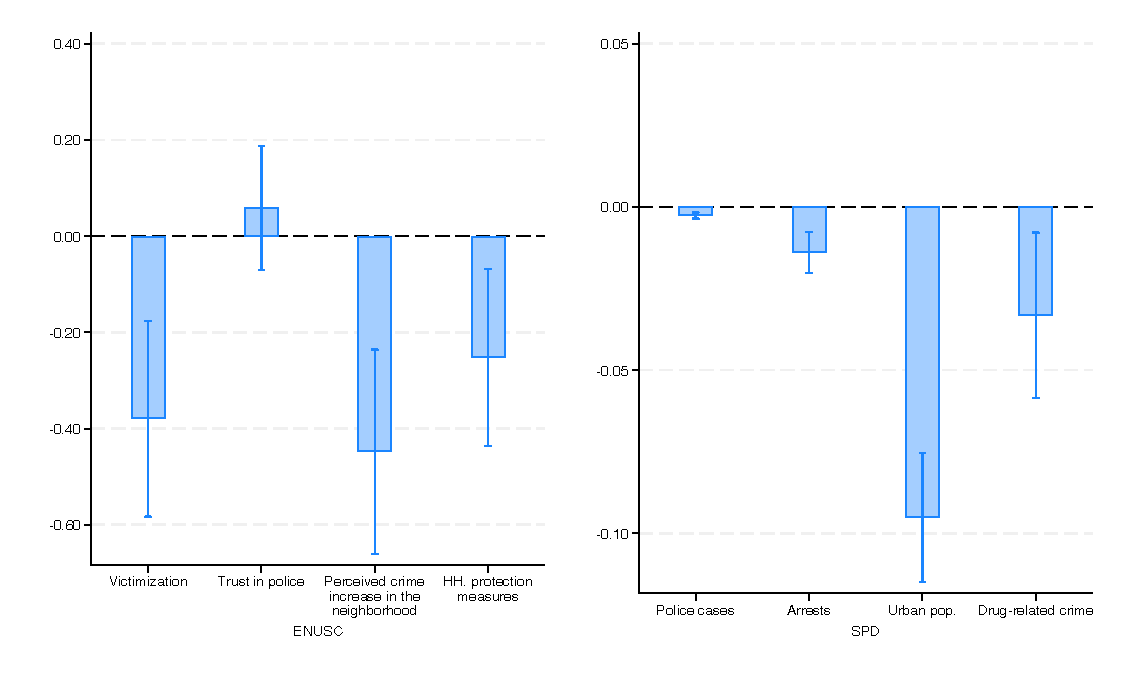
\includegraphics[width=1.1\textwidth]{../manuscript/Graphs/results_predictorsPC_combined.pdf}
 %       \caption{Time of Adoption and Municipality Characteristics}
  %  \end{subfigure}%
    \\[12pt]
    \begin{minipage}{0.95\textwidth}
    \footnotesize Notes: Panel (a) shows the number of municipalities adopting the \emph{Plan Cuadrante} each year (bars), while the circles above them illustrate the cumulative share of the Chilean population living in a municipality with the \emph{Plan Cuadrante} already in place. Panel (b) depicts the metropolitan area of Concepci\'on, the second-largest in Chile: the left map shows its four municipalities---the original police catchment areas---and the right map overlays the Carabineros quadrants together with a kernel-density estimate of all types of robberies and thefts recorded by the police (both reported crimes and arrests). It illustrates how \emph{Plan Cuadrante} subdivided each catchment area (which corresponds to the territory of a municipality) into smaller quadrants, as well as the spatial concentration of crime within them.
    \end{minipage}
\end{figure}
\clearpage

\FloatBarrier

Conceptually, police effectiveness can be viewed as a function of three inputs: total resources, territorial deployment, and policing strategy. Although in some municipalities police resources were increased significantly to operationalize the beat policing model \citep{DIPRES2007_largo,DIPRES2014}, the program primarily transformed the latter two elements. The creation of quadrants was accompanied by permanent geographic assignment of officers to specific areas. This change was operationally critical. By making officers responsible for their quadrant, it encouraged accumulation of local knowledge and stronger community ties, allowing them to adapt patrols and prevention activities to local crime patterns. Importantly, this was not driven by program-specific operational directive changes. Throughout the period we study, a single national set of operational guidelines applied to officers in both treated and control municipalities \citep{Manual_Carabineros2018,DIPRES2007_largo}. Thus, while the average effects we document on crime and crime perception likely reflect combined changes in the three elements we discuss---i.e., resources, deployment, and strategy---the deployment change itself was essential to operationalizing the reform. We discuss the drivers of the effects we document in Section \ref{mechanisms}.

Quadrant size and shape were determined by local police authorities based on factors such as road networks, geographic features, and available resources. In principle, resource allocation across quadrants followed demand for police services, measured in Equivalent Surveillance Units (UVEs); in practice, the station commander retained discretionary authority, as was also the case prior to \emph{Plan Cuadrante} \citep{DIPRES2014}. Municipalities implementing \emph{Plan Cuadrante} were subdivided into an average of seven quadrants, each typically staffed by approximately three officers per shift. On average, each quadrant covered 185 square kilometers and served 13,466 inhabitants. Panel (b) of Figure \ref{fig:figure01} illustrates this structure, showing the 29 quadrants created across the four municipalities of the Concepción metropolitan region---Chile's second-largest metropolitan area and the largest in our sample. Quadrants represented approximately 14\% of the original \emph{comisar\'ia} territory. Officers continued to operate from the same police station but were permanently assigned to a specific sub-area within its jurisdiction. While Carabineros' hierarchical structure limits frontline officer decision-making authority, each quadrant was assigned a Quadrant Delegate (\textit{Delegado de Cuadrante}), a non-commissioned officer, responsible for immediate operational decisions within the quadrant.

\emph{Plan Cuadrante} may affect public safety through two complementary channels: deterrence and police effectiveness, understood as the capacity to respond to and resolve crimes. The changes induced by \emph{Plan Cuadrante}---permanently assigning officers to well-defined neighborhoods and, in some municipalities, increasing available resources---can increase both police visibility and local knowledge. As officers repeatedly patrol the same area, they become familiar with its streets, residents, and routines, which can raise the perceived probability of identification and apprehension and reduce the expected returns to crime. At the same time, this deeper knowledge of local territory and communities can improve police response and case resolution once crimes occur. The reform therefore likely affects both dimensions. Consistent with this interpretation, in Section \ref{results} we document declines in victimization and in reported crime---patterns consistent with deterrence---together with increases in arrests, consistent with improved police effectiveness.

Although beat policing shares features with other policing approaches, such as hot-spot policing and community-based policing, which have been widely studied, it has distinctive features that make it worth studying as an independent approach. Hot-spot policing concentrates resources in high-crime areas and does not focus on building local knowledge and community ties. It is typically implemented through targeted interventions at specific locations rather than systematic territorial organization, and the same officers are not necessarily sent repeatedly to the same areas. Evidence on hot-spot policing is mixed, with some studies showing crime reductions in targeted areas but also potential displacement effects \citep{SR_1}. \emph{Plan Cuadrante}, by contrast, subdivided all urban municipalities into quadrants with permanent officer assignment. As Panel (b) of Figure \ref{fig:figure01} illustrates, some quadrants contained crime hot-spots, but many did not. The reform thus addressed entire urban territories rather than specific high-crime areas, potentially mitigating displacement effects associated with hot-spot policing.

Community-based policing emphasizes building relationships with residents and addressing underlying social issues, and typically involves active community participation in defining strategy and priorities---in some cases, even assuming surveillance and prevention responsibilities. While increasing trust in the police and strengthening community ties were among the declared goals of \emph{Plan Cuadrante}, and may have resulted from its territorial reorganization, the community was not formally involved in the provision of security.\footnote{The \emph{Plan Cuadrante}'s original design contemplated a formal community integration model (MICC) with a Community Affairs Office (\textit{Oficina de Asuntos Comunitarios}) and a dedicated officer in each police station. However, this model was not implemented during our study period. Independent program evaluations from the Budget Office document that these Community Affairs Offices did not exist and had no dedicated personnel, budget, or structured activities in the period we study \citep{DIPRES2007_largo,DIPRES2014}. The community integration model was piloted in four police stations during 2012--2013, none of which are in our analytical sample. Financing was then discontinued in early 2014 and only restored and expanded after our study period ends.}%
 %Similarly, Operations Offices (\textit{Oficina de Operaciones}) formally assigned crime analysis functions but relied on paper-based entry systems, lacking digital infrastructure, analysts, or centralized data systems throughout the study period \citep{DIPRES2014}. Both the community integration model and crime analysis function were substantively implemented only with \emph{Plan Cuadrante} 2.0 (2015--2017) \citep{Carabineros2018}, outside our study period.}

In recent decades, police departments worldwide have transitioned toward beat policing reforms \citep{NASEM2018,PCSP2014}, yet the effectiveness of this model has not been rigorously assessed. Although the beat policing approach introduced through \emph{Plan Cuadrante} shares features with programs previously studied in the economic literature, its distinctive characteristics---comprehensive territorial reorganization and systematic local officer specialization---make it a valuable case for studying how deployment and policing strategies not yet examined in the economics literature affect crime and crime perception.

}
\end{adjustwidth}

We also include below Section 4.4, which summarizes the analyses disentangling the role of resources from that of the beat policing component discussed above:\\

\begin{adjustwidth}{2em}{0em}
{\setcounter{figure}{3}\renewcommand{\thefigure}{\arabic{figure}}
%\textbf{4.4 What Is Driving the Effects of \emph{Plan Cuadrante}?}


To reduce crime and improve security perceptions, police forces need to strengthen both prevention and police effectiveness. Both margins can be shaped by resources, territorial deployment, and policing strategy. This section examines which components of \emph{Plan Cuadrante} are most likely to drive the effects documented in Section \ref{results}. 

The central objective of \emph{Plan Cuadrante} was to introduce a beat policing model by reorganizing deployment. Police operational territories that had typically matched municipal boundaries were subdivided into quadrants, and officers were permanently assigned to these quadrants. During our study period, national operational guidelines remained the same in adopting and non-adopting municipalities. Still, this new deployment likely affected policing strategy at a more operational level, because it allowed officers to adapt patrol routes, schedules, and prevention practices using the local knowledge that the program sought to build.

Although changes in resources were not the core of the reform, implementation contemplated increases in municipalities that lacked the personnel and patrol capacity required to move to this model. During the period we study, Chile was expanding public spending on security, and police resources increased in most municipalities regardless of whether or when they adopted \emph{Plan Cuadrante}. On average, however, municipalities adopting the program experienced larger increases in officers and patrol vehicles, as shown in panels (a) and (b) of Figure \ref{fig:resources}. Since increases in police resources have been shown to reduce crime in some contexts \citep{Evans}, this pattern raises a central question for interpretation, namely whether our estimates reflect resource expansion or the deployment and strategy changes introduced by \emph{Plan Cuadrante}. We address this question through a set of exercises that exploit heterogeneity in resource increases across municipalities and over time.

\FloatBarrier
%--- Implementation
\begin{figure}[H]
    \centering
    \caption{Plan Cuadrante and Changes in Police Resources}
    \label{fig:resources}
    \label{fig:figure_resources}
    \begin{tabular}{cc}
        \begin{minipage}[t]{0.48\textwidth}
            \centering
            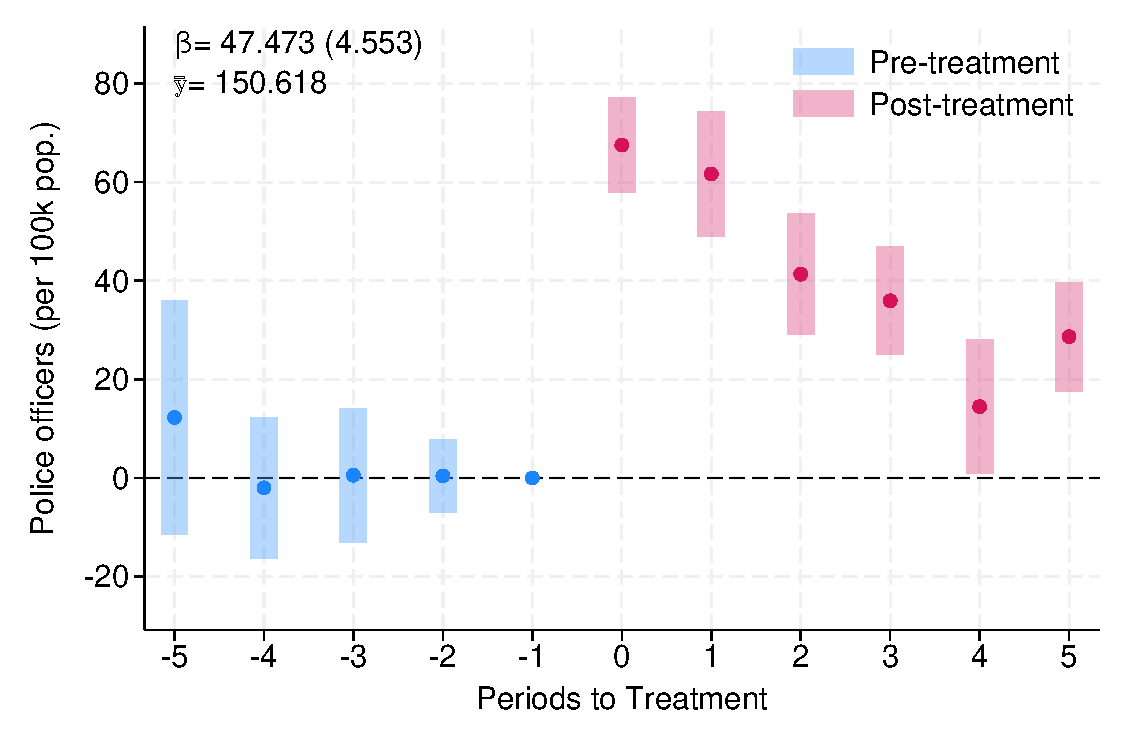
\includegraphics[width=\linewidth]{../manuscript/Graphs/fig4_officers.pdf}

            \small (a) Effect on the number of police officers
        \end{minipage}
        &
        \begin{minipage}[t]{0.48\textwidth}
            \centering
            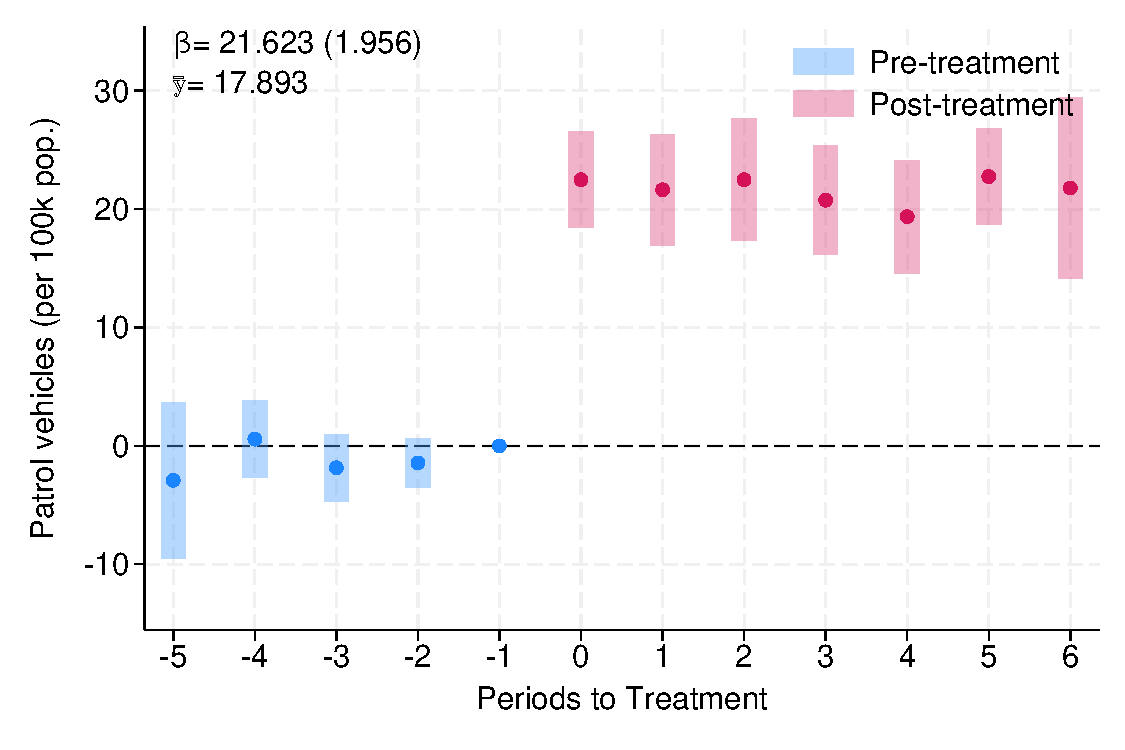
\includegraphics[width=\linewidth]{../manuscript/Graphs/fig4_patrols.pdf}

            \small (b) Effect on the number of patrol vehicles
        \end{minipage}
        \\[4pt]
        \begin{minipage}[t]{0.48\textwidth}
            \centering
            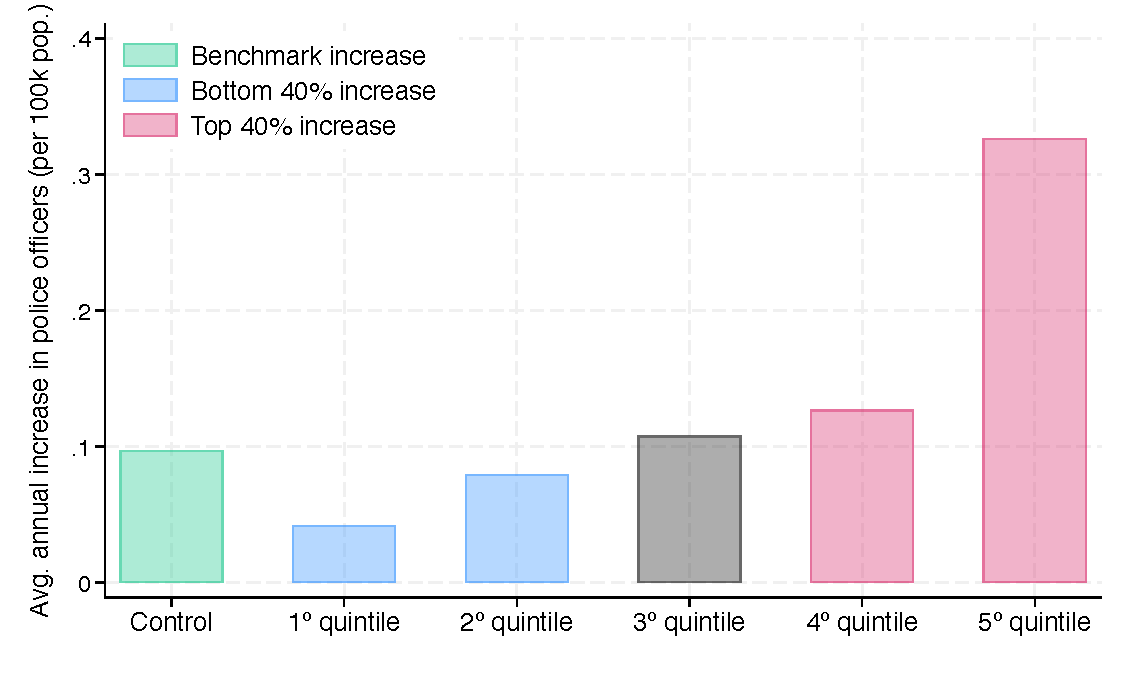
\includegraphics[width=\linewidth]{../manuscript/Graphs/increase_enusc_off_quintiles.pdf}

            \small (c) Distribution of $\Delta$ in police officers
        \end{minipage}
        &
        \begin{minipage}[t]{0.48\textwidth}
            \centering
            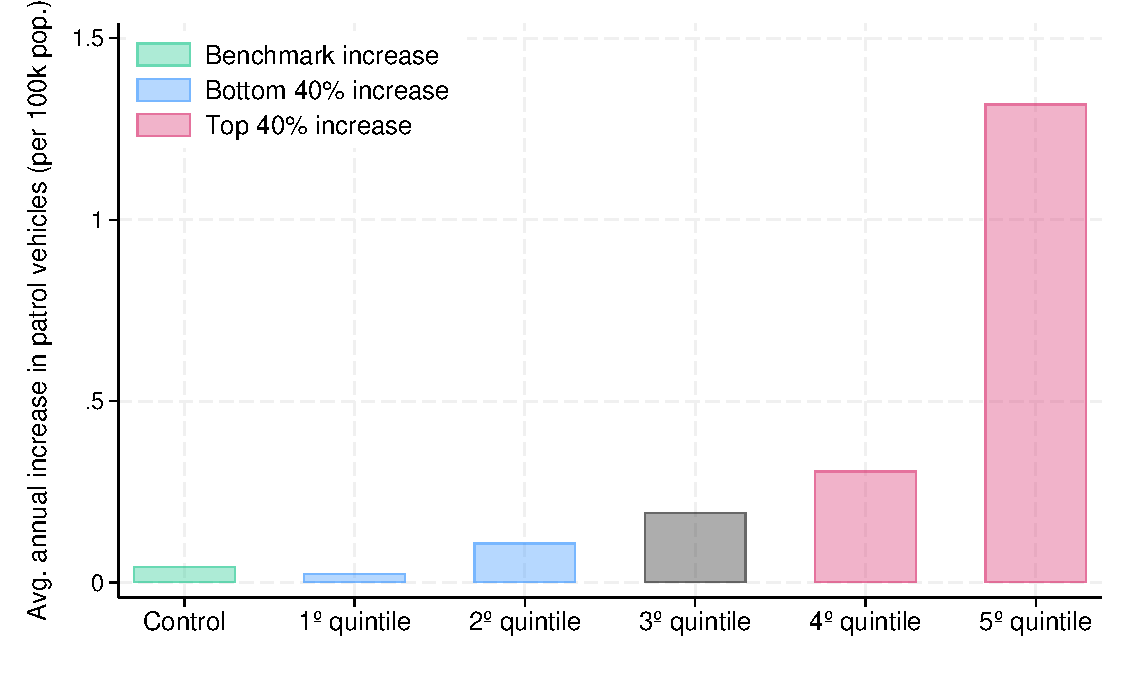
\includegraphics[width=\linewidth]{../manuscript/Graphs/increase_enusc_pv_quintiles.pdf}

            \small (d) Distribution of $\Delta$ in patrol vehicles
        \end{minipage}
        \\[4pt]
        \begin{minipage}[t]{0.48\textwidth}
            \centering
            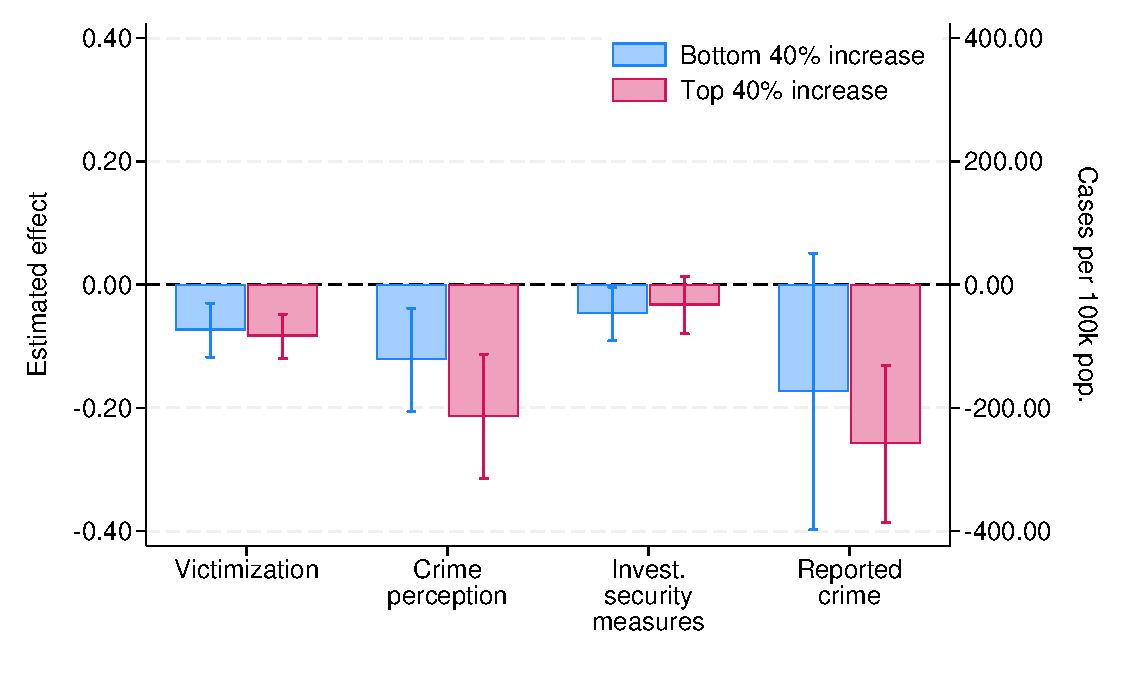
\includegraphics[width=\linewidth]{../manuscript/Graphs/heterogeneity_off.pdf}

            \small (e) Effects by the intensity of $\Delta$ in police officers
        \end{minipage}
        &
        \begin{minipage}[t]{0.48\textwidth}
            \centering
            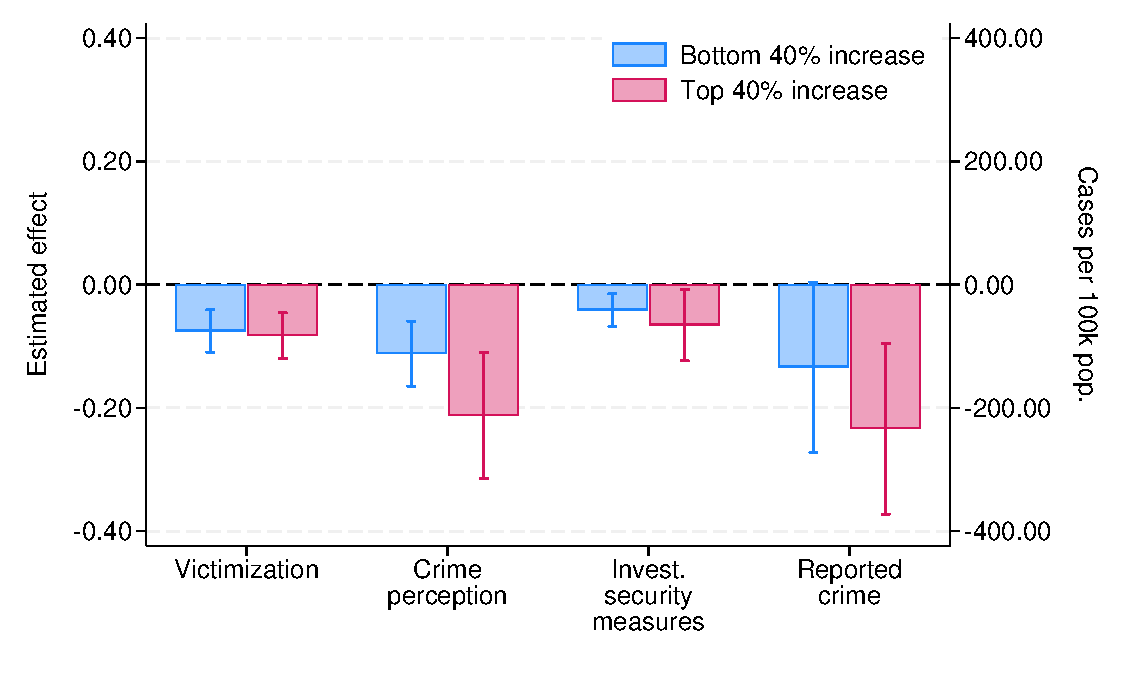
\includegraphics[width=\linewidth]{../manuscript/Graphs/heterogeneity_pv.pdf}

            \small (f) Effects by the intensity of $\Delta$ in patrol vehicles
        \end{minipage}
    \end{tabular}
    \vspace{4pt}
    \begin{minipage}{0.99\textwidth}
    \footnotesize Notes: Panels (a) and (b) show the effect of \emph{Plan Cuadrante} on police officers and patrol vehicles per 100,000 inhabitants. Panels (c) and (d) show the distribution of annual changes in officers and patrol vehicles across municipalities. Panels (e) and (f) report effects by the intensity of resource changes, comparing municipalities in the bottom 40\% and top 40\% of the distribution. The estimation follows \citet{Callaway}. The graphs display estimated coefficients and 95\% confidence intervals. Standard errors are clustered at the municipality level using wild bootstrapping.
    \end{minipage}
\end{figure}
\FloatBarrier
Panels (c) and (d) of Figure \ref{fig:resources} show that the average increase in police resources masks substantial heterogeneity. Municipalities in the bottom 40\% of the resource-change distribution (blue bars) experienced increases close to the average annual variation observed among never treated and not-yet-treated municipalities (green bar). By contrast, municipalities in the top 40\% (red bars) experienced much larger increases, with officers rising by around 22\% and patrol vehicles by around 80\%. If the effects of \emph{Plan Cuadrante} were driven by resource increases alone, we would not expect effects in municipalities whose resource increases were similar to those of the control group. Yet panels (e) and (f) of Figure \ref{fig:resources} show sizeable effects for most crime and crime-perception outcomes even in that low-increase group. While there may be a resource gradient for some crime-perception outcomes, the effects on twelve-month victimization and private investment in security among municipalities with control-like resource increases are close in magnitude to those in municipalities with larger increases. Reassuringly, municipalities in the top and bottom 40\% of the resource-increase distribution do not display differential pre-treatment trends in outcomes or police resources, which suggests that this heterogeneity is not driven by differential pre-existing trends.\footnote{We test for the joint significance of the pre-treatment coefficients between the two groups, separately for the split based on the increase in police officers and the split based on the increase in patrol vehicles. The resulting p-values are, respectively, 0.823 and 0.048 for victimization, 0.059 and 0.379 for crime perception, 0.820 and 0.157 for investment in security measures, and 0.213 and 0.419 for reported crime, as well as 0.616 and 0.444 for police officers and 0.405 and 0.157 for patrol vehicles.}

Although we cannot fully separate the beat policing component from the resource component of the reform---resources may have been important to enable effective implementation of the program, or may explain part of the effects in some municipalities---the fact that municipalities with resource increases similar to those experienced by control municipalities still display sizeable effects indicates that the effects of \emph{Plan Cuadrante} are not driven entirely by resources.\footnote{We also re-estimate the results in Figure \ref{fig:figure02} but controlling for police resources. Online Appendix Table \ref{tab:results_controlbyresources} shows that the magnitude of the estimated effects remains similar for most variables, although the statistical significance is reduced in some estimations. This likely reflects a mechanical feature of the \citet{Callaway} estimation procedure: control variables are not incorporated parametrically, but are instead used to construct the comparison group via outcome regression or propensity-score weighting, so the resulting estimation uncertainty propagates to the ATT standard errors. Note, in addition, that police resources are a bad control---i.e., at least part of their variation is a result of the adoption of \emph{Plan Cuadrante}---so these results should be interpreted cautiously.}\footnote{Table \ref{tab:resourcecorrelates} in Online Appendix \ref{sec:appendixB} examines which factors are associated with a larger increase in police resources upon the adoption of \emph{Plan Cuadrante}.}


\FloatBarrier
%--- Implementation
\begin{figure}[h!]
    \centering
    \caption{Police Resources and Public Safety}
    \label{fig:resources2}
    \begin{subfigure}[t]{0.55\textwidth}
        \centering
        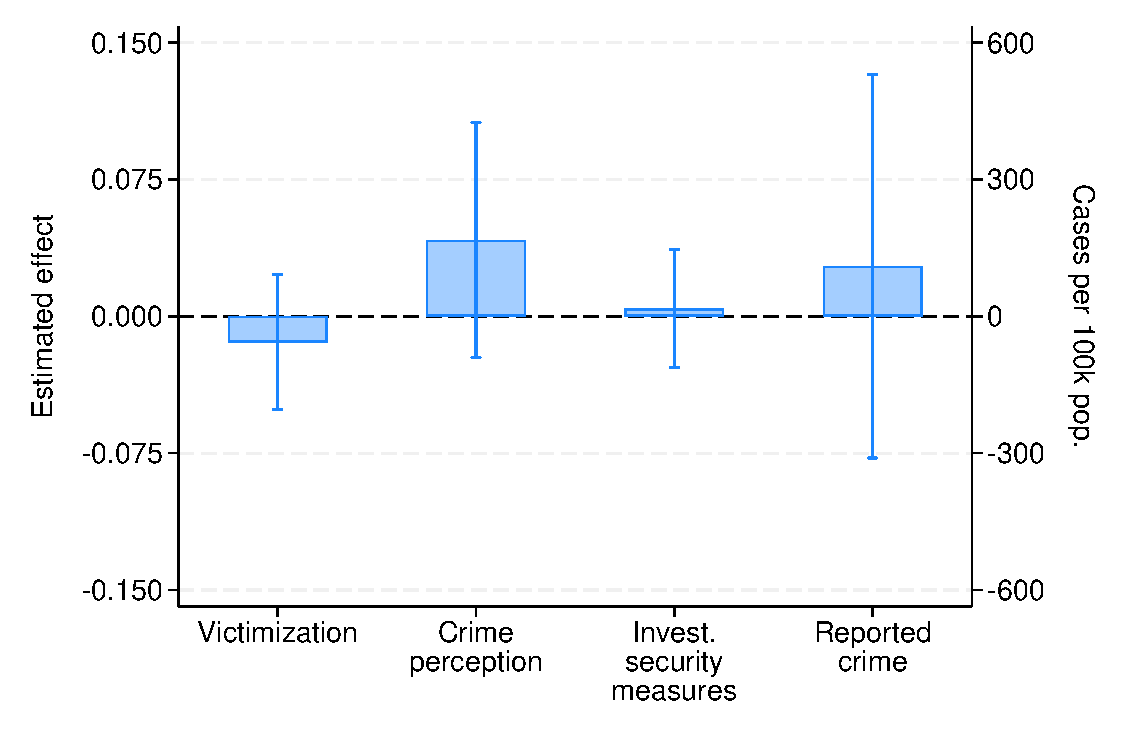
\includegraphics[width=\linewidth]{../manuscript/Graphs/results_SC_att_combined.pdf}
        \caption{Effects of \emph{Seguridad Ciudadana}}
    \end{subfigure}
    \\[6pt]
    \begin{subfigure}[t]{0.55\textwidth}
        \centering
        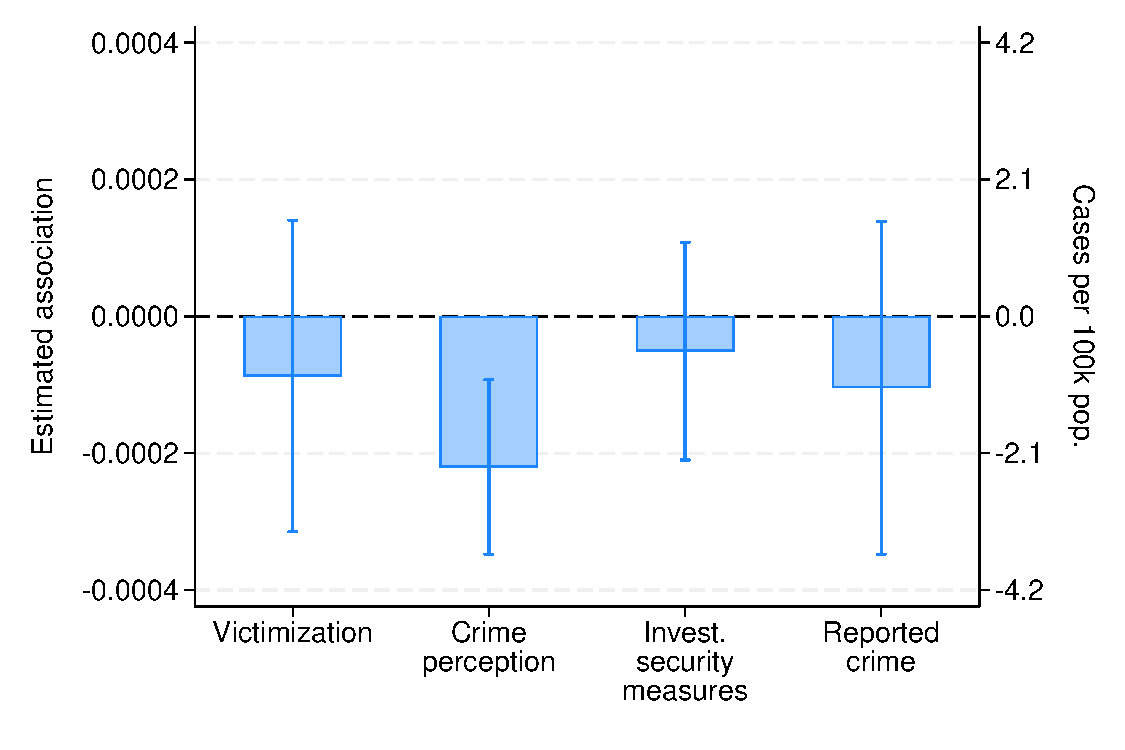
\includegraphics[width=\linewidth]{../manuscript/Graphs/results_corr_novariation_off_santiago.pdf}
        \caption{Association between police officers and effectiveness}
    \end{subfigure}
    \\[6pt]
    \begin{subfigure}[t]{0.55\textwidth}
        \centering
        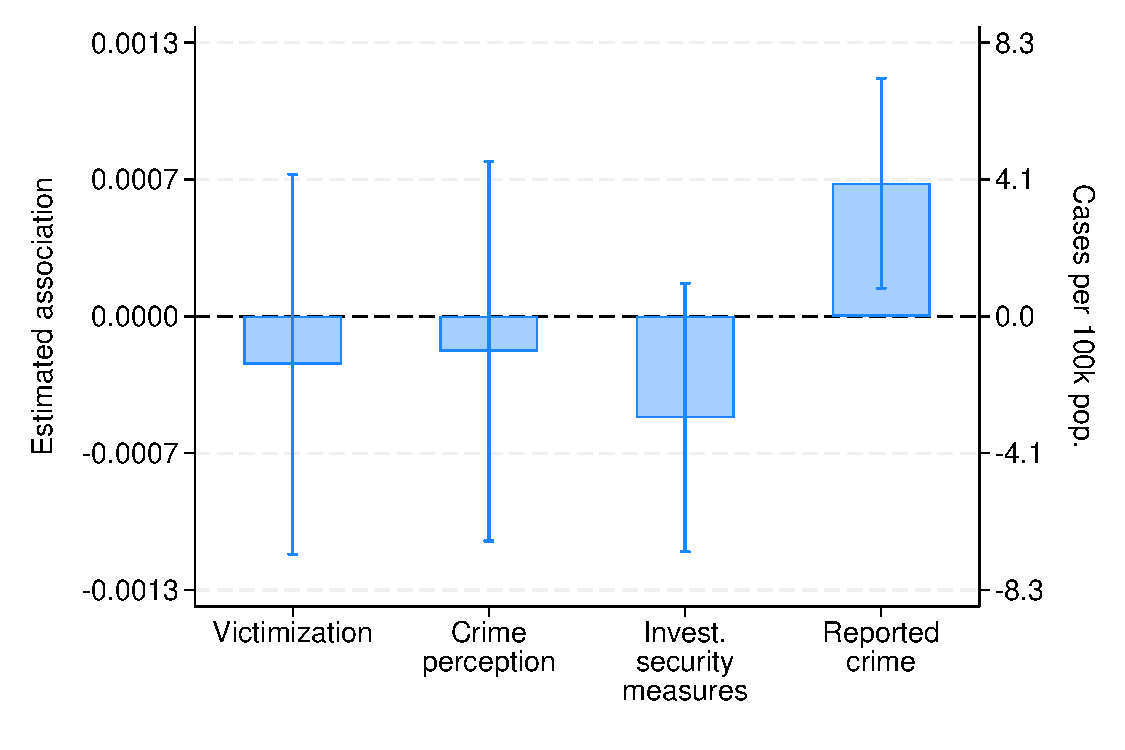
\includegraphics[width=\linewidth]{../manuscript/Graphs/results_corr_novariation_veh_santiago.pdf}
        \caption{Association between patrol vehicles and effectiveness}
    \end{subfigure}
    \\[8pt]
    \begin{minipage}{0.99\textwidth}
    \footnotesize Notes: Panel (a) reports the pooled effect of \emph{Seguridad Ciudadana}, a program that expanded local security personnel to support patrolling and deterrence but did not replicate the deployment-and-strategy features of \emph{Plan Cuadrante}. Panels (b) and (c) report within-municipality associations between police resources and police-effectiveness outcomes among the 41 municipalities of the Santiago Metropolitan Region, all of which had adopted \emph{Plan Cuadrante} by 2000. The regressions include municipality and year fixed effects. Standard errors are clustered at the municipality level using the wild bootstrapping procedure.
    \end{minipage}
\end{figure}
\FloatBarrier

To further investigate whether resource increases alone can explain our results, we assess the effects of \emph{Seguridad Ciudadana}, a program that expanded local security personnel to support patrolling and deterrence, but did not replicate the core deployment-and-strategy features of \emph{Plan Cuadrante}. Using a difference-in-differences specification following \citet{Callaway}, panel (a) of Figure \ref{fig:resources2} shows no significant effects of these resource changes on police effectiveness. Further details about this exercise and the corresponding event-study estimates are reported in Online Appendix \ref{sec:appendixB} and Online Appendix Figure \ref{fig:figureA5}. 


Finally, we study whether variation in police resources in municipalities that had already adopted \emph{Plan Cuadrante} improves public safety and security perceptions. Using ENUSC data and information on resources for 2006--2012 in the 41 municipalities of the Santiago Metropolitan Region---all of which had adopted \emph{Plan Cuadrante} by 2000---we exploit variation in officers and patrol vehicles that is unrelated to program adoption. Panels (b) and (c) of Figure \ref{fig:resources2} show the association between police resources and our main outcomes, conditional on municipality and year fixed effects. With one exception---the association between police officers and crime perception---none of these associations is statistically significant at conventional confidence levels. \footnote{Online Appendix Figure \ref{fig:figureA7B} reports the same exercise and also shows similar results for the broader set of municipalities that adopted \emph{Plan Cuadrante} before 2006 and never-treated municipalities (red bars); see Online Appendix \ref{sec:appendixB} for further details.}

Taken together, these results suggest that resource increases alone do not account for the effects of \emph{Plan Cuadrante}. We next turn to evidence that speaks more directly to the beat-policing components of the reform.

Panel (a) of Figure \ref{fig:police_performance} shows that, following the adoption of \emph{Plan Cuadrante}, households are much more likely to report increased police presence in their neighborhoods. The share of households perceiving increased police presence rises by 35 percentage points (156\%), the share reporting that police pass by their house daily rises by 22 percentage points (59\%), the share reporting never seeing police patrols near their house falls by 10 percentage points (57\%), and complaints about lack of police surveillance fall by around 5 percentage points (20\%). This evidence is consistent with both larger resources and the new deployment model. Yet the latter estimate---the only police-presence outcome for which we can separately estimate effects in municipalities with small and large resource increases---is similar in magnitude across the two groups, which suggests that the increase in police presence is not explained only by larger resource increases (see Online Appendix Figure \ref{fig:heterogeneity_appendix}).\footnote{We cannot estimate heterogeneous effects for other police-presence outcomes, such as the reporting of police passing by or the share of households perceiving an increase in police presence, because those variables are available only in ENUSC rounds 2003, 2005, and 2006, while resource data start in 2006.} More importantly, the broader pattern of results suggests that \emph{Plan Cuadrante} did more than simply increase patrolling intensity. Existing work shows that police presence can reduce crime while officers are present, but that its overall effects may be attenuated when crime is displaced across places or time windows \citep{MASTROBUONI2019, Blanes_Mastrobuoni_2018}. Our results point to something broader. As discussed in Section \ref{results}, we find actual declines in victimization and reported crime, together with no evidence of spillovers to neighboring municipalities. This pattern is more consistent with officers accumulating local knowledge and adapting prevention strategies to local conditions under stable territorial assignment than with a purely mechanical increase in patrol intensity.

Panel (b) of Figure \ref{fig:police_performance} reinforces this interpretation. Households in early-adopting municipalities report better police performance across multiple dimensions. They are 8.1 percentage points (16\%) more likely to rate police performance as good or very good, 7.6 percentage points (11\%) more likely to describe police as efficient, 5 percentage points (6\%) more likely to report that police are helpful, and 4.9 percentage points (7\%) more likely to report that police are well informed. They are also 3.9 percentage points (10\%) less likely to perceive police as corrupt, 7.9 percentage points (21\%) less likely to believe police fail to control crime, and 7.6 percentage points (22\%) less likely to report that police do not perform their duties effectively.\footnote{Information on police performance is only available in ENUSC round 2005. Using this round, we compare perceived police performance in municipalities that adopted \emph{Plan Cuadrante} in 2005 or earlier and in municipalities adopting after 2005. Figure \ref{fig:balance_doseresponse} in Online Appendix \ref{sec:appendixB} shows that the number of years of exposure to \emph{Plan Cuadrante} is positively correlated with perceived police performance. While these exercises on perceived police performance should be interpreted with caution, we show in the same appendix that the timing of future adoption is not correlated with perceived police performance in 2005 for municipalities that had not yet adopted the program by 2005.} %These perceived improvements are consistent with a setting in which officers become better informed about local routines and more effective in how they patrol and respond.

The administrative evidence points in the same direction. Panel (c) of Figure \ref{fig:police_performance} shows that arrests per 100,000 inhabitants increase by 48 (14\%) in our main estimates, even as crime declines overall.\footnote{As with reported crime, this event study is restricted to 5 pre-treatment and 7 post-treatment periods for symmetry with the ENUSC-based analysis; Online Appendix Figure \ref{fig:admin_uncapped} reports the results for arrests using the full set of pre-treatment and post-treatment periods.} This effect is also significant among municipalities with resource increases similar to those in the control group (see Online Appendix Figure \ref{fig:heterogeneity_appendix}). Consistent with this pattern, panel (d) of Figure \ref{fig:police_performance} shows that the arrest rate per reported crime also increases by 1.7 percentage points (10\%), suggesting that a higher share of crimes reported to the police are being solved. Because these gains appear even where resources did not increase more than in control municipalities, they are difficult to reconcile with a pure resource story and are more naturally interpreted as improvements in police effectiveness under the deployment and strategy changes introduced by \emph{Plan Cuadrante}. The corresponding event-study estimates for arrests, the arrest rate per reported crime, and trust in the police in Figure \ref{fig:police_performance} confirm that these changes emerge only after adoption.

Finally, panel (e) of Figure \ref{fig:police_performance} shows a sharp increase in trust in the police in our main specification (Section \ref{results}), consistent with one of the objectives of beat policing, namely bringing officers closer to the community and allowing them to accumulate local knowledge through repeated interaction. Online Appendix Figure \ref{fig:heterogeneity_appendix} shows that this effect remains sizeable both in municipalities that experienced resource increases similar to the control group and in those with larger increases.

Overall, although resources were likely important for implementation and may explain part of the effects in some municipalities, the results in this section indicate that resource changes alone are not enough to explain our findings. The evidence is more consistent with a combination of deployment changes and the strategy adjustments enabled by local knowledge accumulation under permanent assignment to quadrants.

\FloatBarrier
%--- Implementation
\begin{figure}[!ht]
    \centering
    \caption[\emph{Plan Cuadrante} and Changes in Police Performance]{\emph{Plan Cuadrante} and Changes in Police Performance}
    \label{fig:figure05}
    \label{fig:police_performance}
    \label{fig:effectiveness_es}
    \begin{subfigure}[t]{0.44\textwidth}
        \centering
        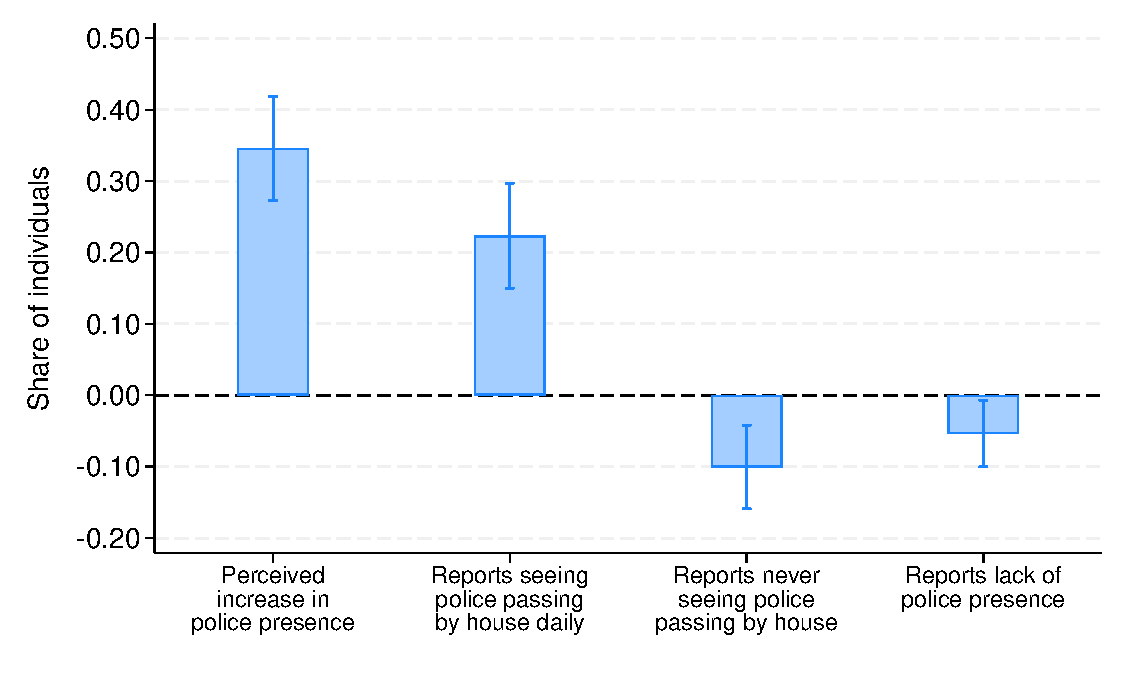
\includegraphics[width=\linewidth]{../manuscript/Graphs/results_policepresence.pdf}
        \caption{Effect on police presence}
    \end{subfigure}\hfill
    \begin{subfigure}[t]{0.44\textwidth}
        \centering
        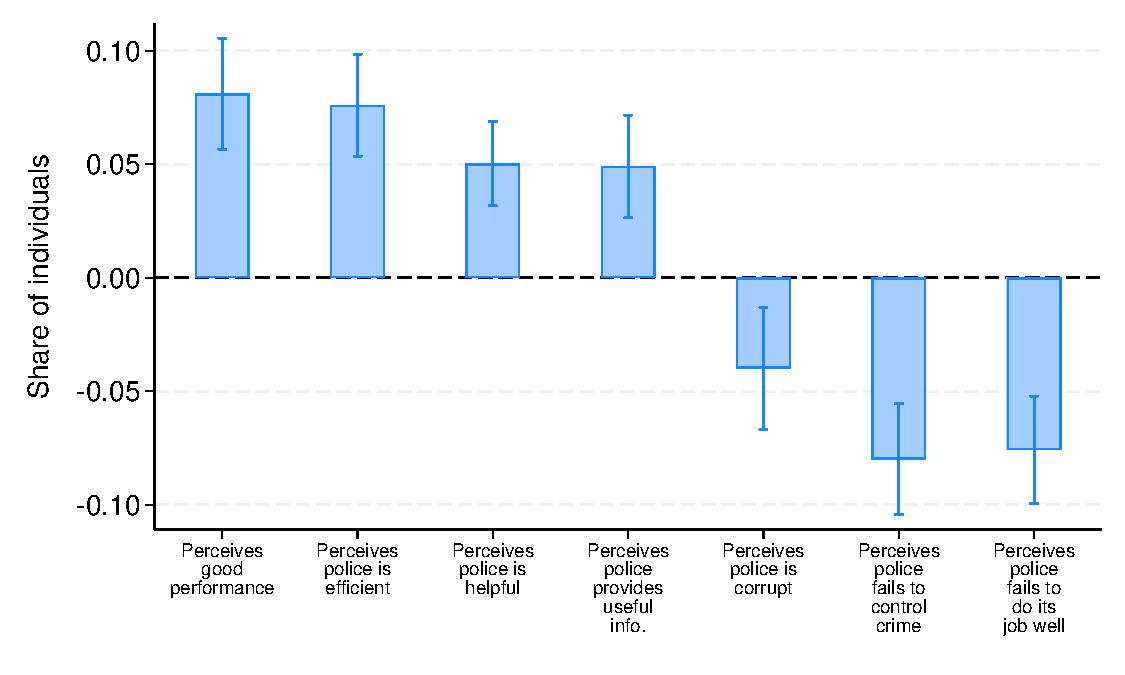
\includegraphics[width=\linewidth]{../manuscript/Graphs/combined_PCttest_2.pdf}
        \caption{Effect on perceived police performance}
    \end{subfigure}
    \\[6pt]
    \begin{subfigure}[t]{0.44\textwidth}
        \centering
        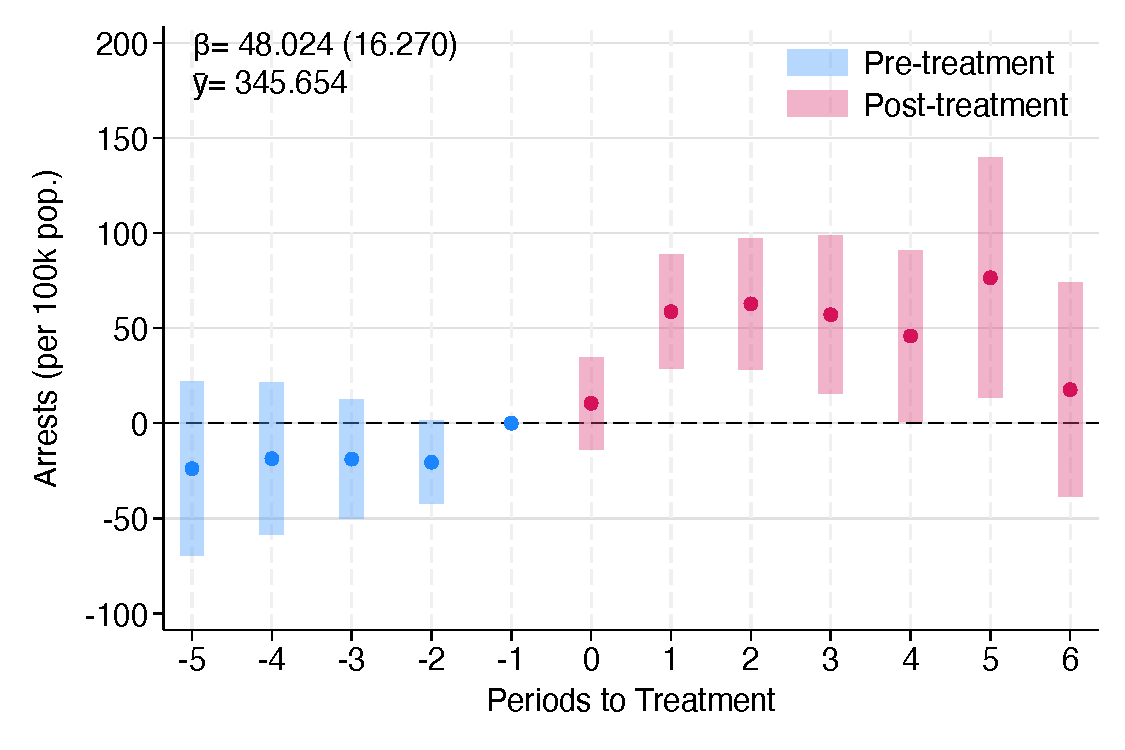
\includegraphics[width=\linewidth]{../manuscript/Graphs/totalarrestscrime_allcomunas.pdf}
        \caption{Arrests (per 100k pop.)}
    \end{subfigure}\hfill
    \begin{subfigure}[t]{0.44\textwidth}
        \centering
        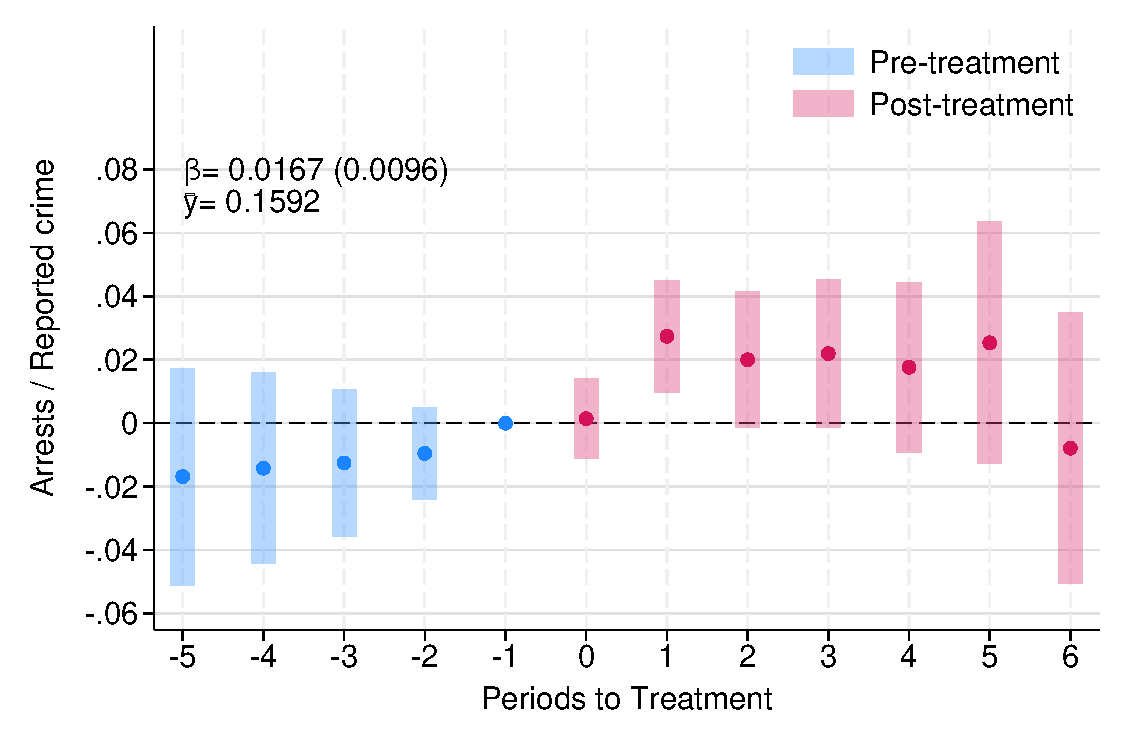
\includegraphics[width=\linewidth]{../manuscript/Graphs/arrests_over_reportedcrime_allcomunas.pdf}
        \caption{Arrests / Reported crime}
    \end{subfigure}
    \\[6pt]
    \begin{subfigure}[t]{0.44\textwidth}
        \centering
        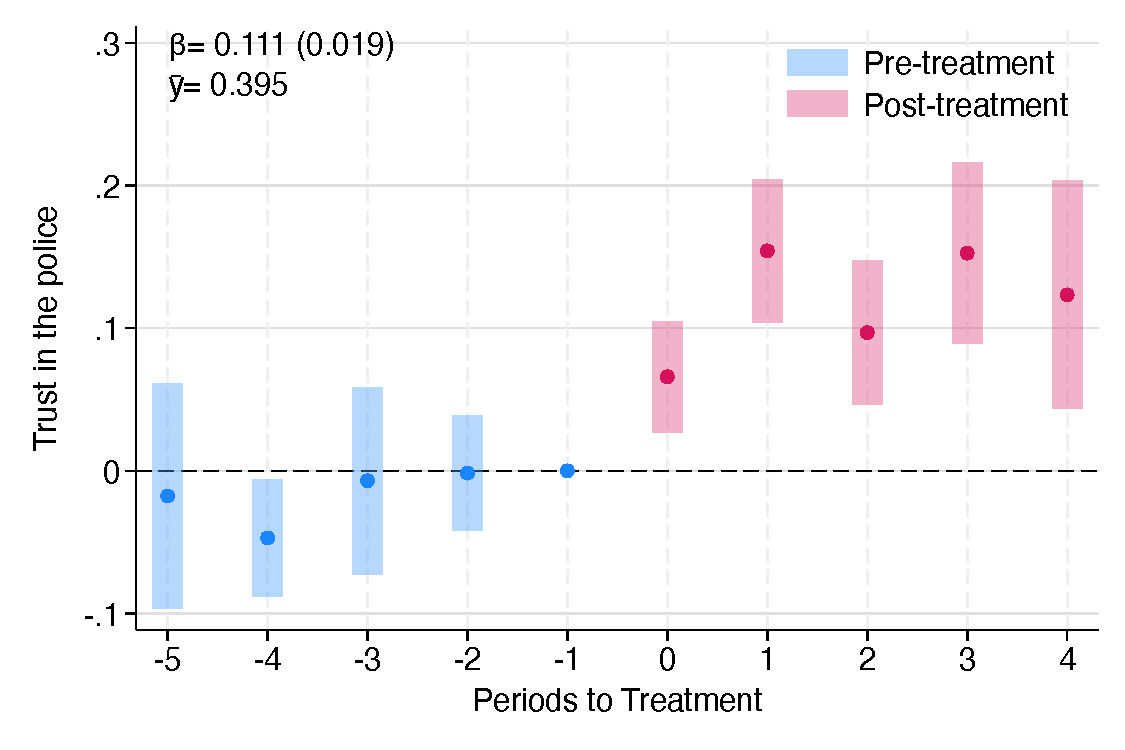
\includegraphics[width=\linewidth]{../manuscript/Graphs/results_trustcarabineros.pdf}
        \caption{Trust in the police}
    \end{subfigure}
    \\[8pt]
    \begin{minipage}{0.99\textwidth}
    \footnotesize Notes: Panel (a) reports the effects on perceived police presence. Panel (b) reports perceived police performance in 2005, comparing municipalities where \emph{Plan Cuadrante} was already implemented before 2006 with municipalities where it was implemented after 2005. Panels (c), (d), and (e) report dynamic event-study estimates for arrests per 100,000 inhabitants, the ratio of arrests to reported crime, and trust in the police. The estimation follows \citet{Callaway}. The graphs display estimated coefficients and 95\% confidence intervals. Standard errors are clustered at the municipality level using the wild bootstrapping procedure.
    \end{minipage}
\end{figure}

\FloatBarrier

%Overall, while resources were arguably important for implementation, the evidence suggests that the beat policing elements---permanent assignment of officers to quadrants and greater local knowledge---were important drivers of the improvements in public safety and security perceptions we document in the paper.



 
}
\end{adjustwidth}

We also added a new Online Appendix B subsection, ``Factors Associated with the Increase in Police Resources,'' regressing the increase in resources at the time of adoption on pre-treatment municipality characteristics. Because the UVE demand-and-supply files were not provided by \textit{Carabineros}, we cannot infer the exact administrative rule used to assign the additional resources:

\begin{adjustwidth}{2em}{0em}
As discussed in Section \ref{institutions} and in Online Appendix \ref{resources_plan_cuadrante}, the increase in police resources associated with the adoption of \emph{Plan Cuadrante} varied substantially across municipalities. In principle, this increase should be related to each municipality's pre-existing police resource deficit---measured in Equivalent Surveillance Units (UVEs)---which \emph{Plan Cuadrante} was meant to help close. However, program evaluations do not clearly establish that this deficit is what determined the size of the resource increase each municipality received \citep{DIPRES2007_largo,DIPRES2014}.\footnote{Although we requested information on the demand and supply of UVEs underlying this allocation, this information was not provided by \textit{Carabineros}.} If the pre-existing deficit is not what determines the resource increase, what is it related to? Reassuringly, municipalities receiving larger versus smaller resource increases do not display differential pre-treatment trends in either the outcomes of interest or in police resources themselves.\footnote{We test for the joint significance of the pre-treatment coefficients between the two groups, separately for the split based on the increase in police officers and the split based on the increase in patrol vehicles. The resulting p-values are, respectively, 0.823 and 0.048 for victimization, 0.059 and 0.379 for crime perception, 0.820 and 0.157 for investment in security measures, and 0.213 and 0.419 for reported crime, as well as 0.616 and 0.444 for police officers and 0.405 and 0.157 for patrol vehicles.} In this section we examine whether the magnitude of the resource increase experienced by a municipality upon adoption is correlated with its pre-treatment levels in crime, police resources, and other observable characteristics. Specifically, we regress the increase in resources at the time of adopting \emph{Plan Cuadrante} on municipality characteristics measured before the program's introduction, including crime and police resources in 2006, the first year for which information on police resources is available. Thus, we restrict this analysis to municipalities that adopted \emph{Plan Cuadrante} from 2007 onward.

Table \ref{tab:resourcecorrelates} reports OLS regressions of the average annual increase in police officers and patrol vehicles per 100,000 inhabitants on pre-adoption municipality characteristics, separately for the administrative (SPD) sample at the municipality level (columns 1--2) and the ENUSC sample at the survey-respondent level (columns 3--4). All variables are standardized and standard errors are clustered by municipality, so coefficients are comparable in magnitude across regressors.

The results provide little support for the hypothesis that municipalities with worse pre-treatment crime outcomes received systematically larger resource increases. Pre-treatment reported crime is, if anything, negatively associated with the subsequent increase in both officers and vehicles in the administrative sample (columns 1--2); in the ENUSC sample, it is negatively associated with the increase in officers (column 3), although it is positively associated with the increase in vehicles (column 4). Pre-treatment victimization is, if anything, negatively associated with both increases in the ENUSC sample (columns 3--4). Pre-treatment arrests, crime perception, trust in the police, and private investment in security measures are not significantly associated with the resource increase. The increase in resources is instead more strongly predicted by structural municipality characteristics: less populous municipalities experienced larger increases in three of the four specifications, and municipalities with higher poverty rates predicted a larger increase in vehicles in the administrative sample (column 2), although this association is not significant for officers in that sample (column 1) or in the ENUSC sample (columns 3--4).
\end{adjustwidth}

\clearpage
\noindent\textbf{Other figures and tables referenced above:}
\vspace{0.5em}

{\setcounter{figure}{1}\renewcommand{\thefigure}{\arabic{figure}}
%--- Implementation
\begin{figure}[h!]
    \centering
    \caption{Effects of \emph{Plan Cuadrante} on Crime Outcomes and Security Perceptions}
    \label{fig:figure02}
    \begin{subfigure}{0.495\textwidth}
        \centering
        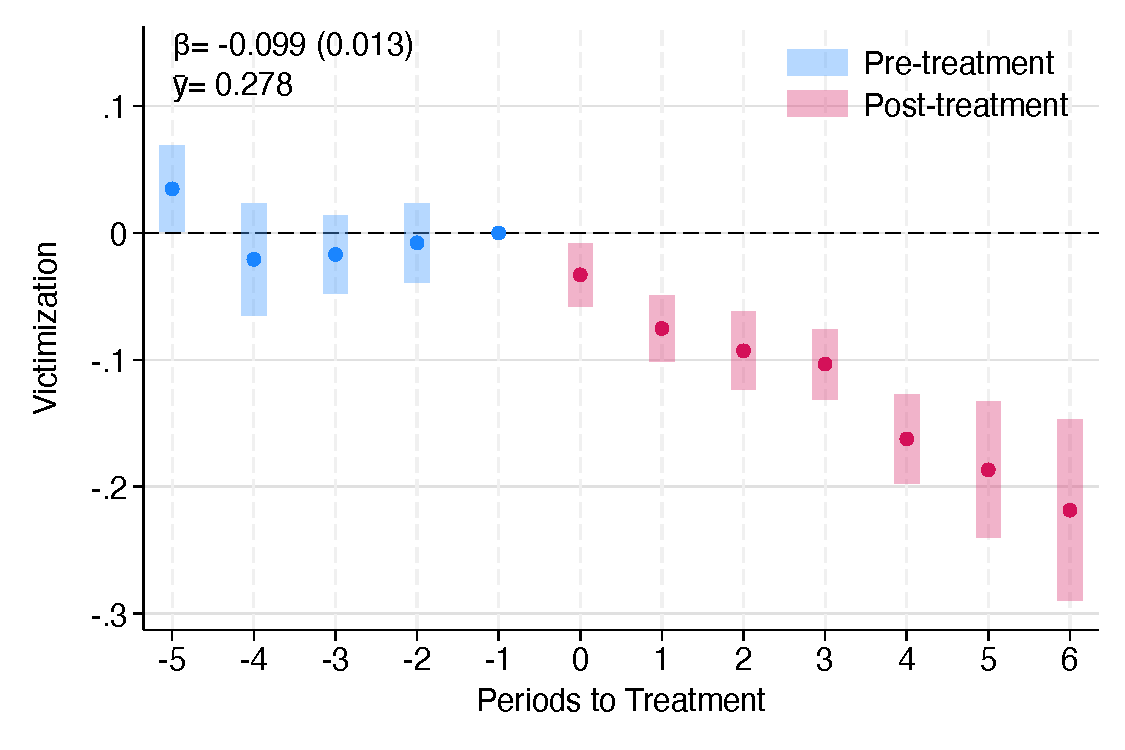
\includegraphics[width=\textwidth]{../manuscript/Graphs/results_victimization.pdf}
        \caption{Victimization in last 12 months}
    \end{subfigure}%
    ~
    \begin{subfigure}{0.495\textwidth}
    \centering
    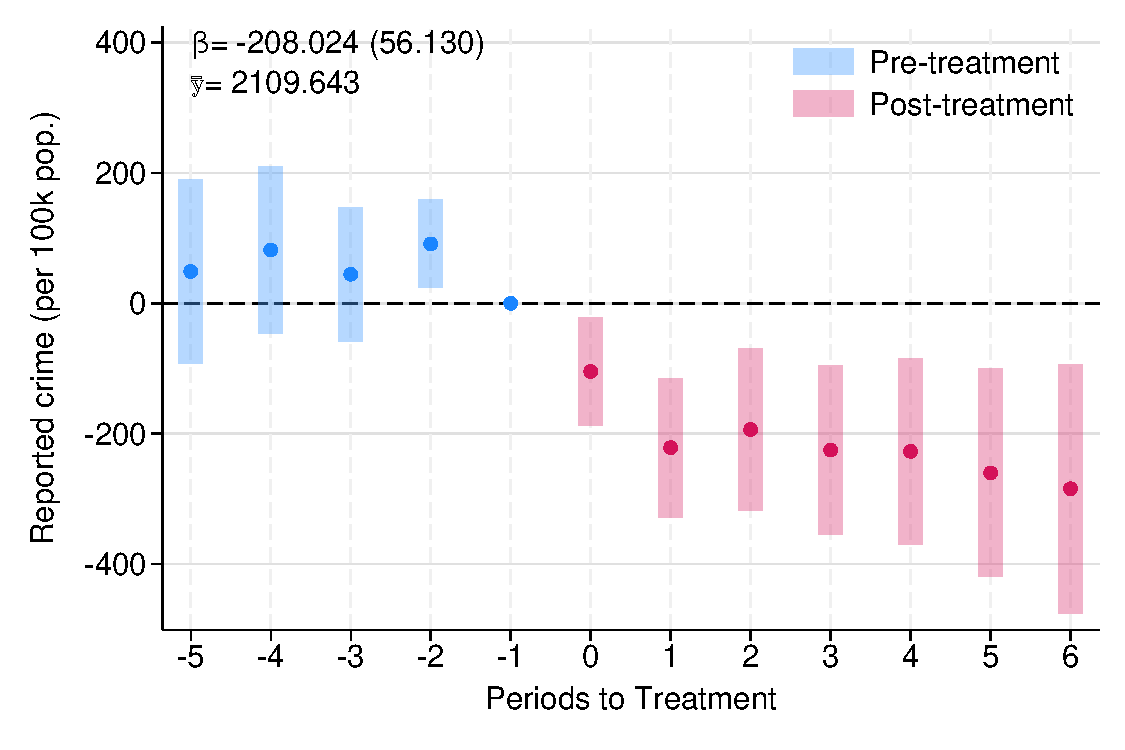
\includegraphics[width=\textwidth]{../manuscript/Graphs/totalreportedcrime_allcomunas.pdf}
        \caption{Reported crime per 100k inhabitants}
    \end{subfigure}
        \begin{subfigure}{0.495\textwidth}
        \centering
        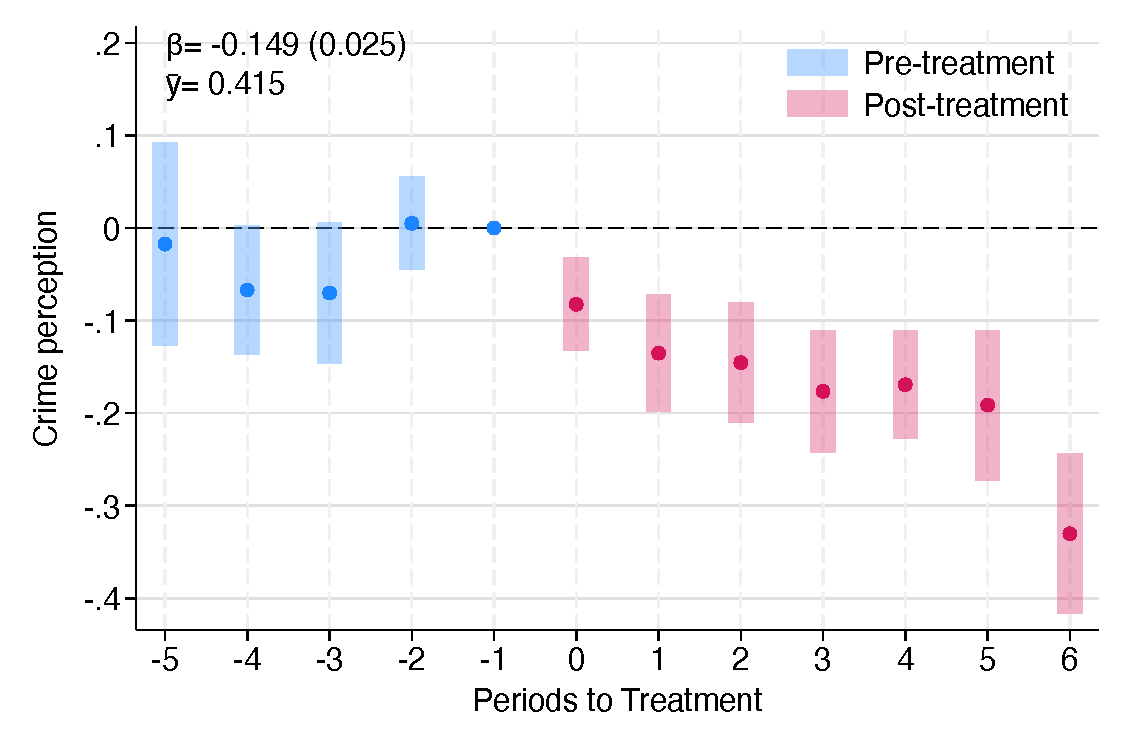
\includegraphics[width=\textwidth]{../manuscript/Graphs/results_perception.pdf}
        \caption{Households reporting an increase in crime}
    \end{subfigure}%
    ~
    \begin{subfigure}{0.495\textwidth}
    \centering
    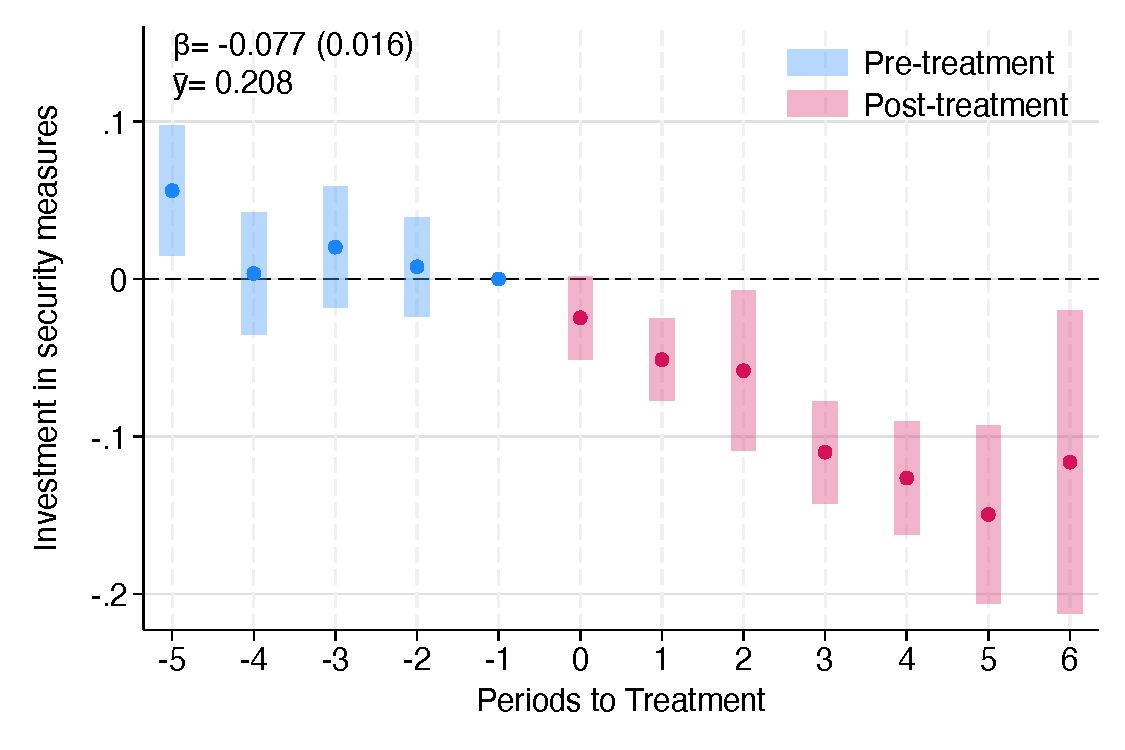
\includegraphics[width=\textwidth]{../manuscript/Graphs/results_hhprotectionmeasures.pdf}
        \caption{Households adopting security measures}
    \end{subfigure}
    \\[12pt]
    \begin{minipage}{0.99\textwidth}
    \footnotesize
    Notes: This figure shows the dynamic effects of the \emph{Plan Cuadrante} on different measures of police effectiveness. The estimation is conducted using the procedure developed in \citet{Callaway} for difference-in-differences with staggered treatment adoption. The dots in the figure represent the estimated coefficients and the bars behind them 95\% confidence intervals. Standard errors are clustered at the municipality level using the wild bootstrapping procedure. The pooled effect and the mean outcome before the introduction of the treatment is also presented in each panel. Panel (a) reports the effect of \emph{Plan Cuadrante} on the probability of household victimization in the last 12 months using the ENUSC survey. Panel (b) reports the effect on the number of crimes reported to the police in the municipality per 100,000 inhabitants using administrative data. Panel (c) reports the effect on the probability of perceiving an increase in crime using the ENUSC survey. Panel (d) reports the effect on the probability of adopting security measures in the last twelve months using the ENUSC survey. Panel (a) includes 93,041 observations; panel (b), 4,231; panel (c), 89,578; and panel (d), 93,041 observations.
    \end{minipage}
\end{figure}
}

\clearpage

{\renewcommand{\thetable}{B.4}
\begin{table}[H]
\centering
\caption{Predictors of the Increase in Police Resources under \emph{Plan Cuadrante}}
\label{tab:resourcecorrelates}
\begin{threeparttable}
\small
\setlength{\tabcolsep}{6pt}
\renewcommand{\arraystretch}{1.1}
\begin{tabular}{@{}l cc cc@{}}
\toprule
& \multicolumn{2}{c}{Administrative sample} & \multicolumn{2}{c}{ENUSC sample} \\
\cmidrule(lr){2-3} \cmidrule(lr){4-5}
& Police & Patrol & Police & Patrol \\
Dep.\ var: avg.\ annual increase & officers & vehicles & officers & vehicles \\
in resources (share of pre-adoption level) & (1) & (2) & (3) & (4) \\
\midrule
Reported crime (per 100k pop.) & $-0.203^{**}$ & $-0.199^{**}$ & $-0.319^{*}$ & $0.272^{*}$ \\
 & (0.099) & (0.097) & (0.182) & (0.137) \\
Arrests (per 100k pop.) & $0.099$ & $-0.041$ & $0.003$ & $0.297$ \\
 & (0.136) & (0.129) & (0.186) & (0.223) \\
Victimization &  &  & $-0.017^{*}$ & $-0.025^{*}$ \\
 &  &  & (0.010) & (0.013) \\
Crime perception &  &  & $0.005$ & $0.008$ \\
 &  &  & (0.017) & (0.014) \\
Trust in the police &  &  & $0.024$ & $0.027$ \\
 &  &  & (0.018) & (0.019) \\
Investment in security measures &  &  & $0.004$ & $-0.003$ \\
 &  &  & (0.010) & (0.009) \\
Police officers (per 100k pop.) & $-0.207$ & $0.155$ & $-0.888^{***}$ & $0.571^{***}$ \\
 & (0.155) & (0.129) & (0.154) & (0.136) \\
Patrol vehicles (per 100k pop.) & $-0.129$ & $-0.139$ & $0.537^{**}$ & $-0.507^{***}$ \\
 & (0.129) & (0.126) & (0.212) & (0.169) \\
Log population & $-0.529^{***}$ & $-0.203^{*}$ & $-0.193$ & $-0.626^{**}$ \\
 & (0.145) & (0.112) & (0.189) & (0.269) \\
Poverty rate (2004) & $0.170$ & $0.308^{**}$ & $0.027$ & $-0.017$ \\
 & (0.113) & (0.126) & (0.108) & (0.108) \\
\midrule
Observations & 65 & 65 & 8,781 & 8,781 \\
R-squared & 0.342 & 0.282 & 0.614 & 0.545 \\
\bottomrule
\end{tabular}
\begin{tablenotes}[flushleft]
\footnotesize
\item \textit{Note:} OLS regressions of the average annual increase in police officers (columns 1 and 3) and patrol vehicles (columns 2 and 4) per 100{,}000 inhabitants, from the year before adoption of \emph{Plan Cuadrante} to 2012. As in panels (a) and (b) of Figure \ref{fig:figure_resources}, the increase is expressed as a share of the resources available the year before adoption. Columns 1--2 use the administrative sample at the municipality level; columns 3--4 use ENUSC survey respondents interviewed before 2007 (survey outcomes at the respondent level, other regressors as pre-2006 municipality aggregates). All variables are standardized. Standard errors clustered by municipality in parentheses.
\item $^{*}p<0.1$; $^{**}p<0.05$; $^{***}p<0.01$.
\end{tablenotes}
\end{threeparttable}
\end{table}
}

\clearpage



\end{response}
\stepcounter{AnsweredComments}


% Comment R2 - 6
\begin{refcomment}

Since the authors emphasize local knowledge as the key mechanism, the paper would also benefit from a deeper integration with the economics literature on local governance and institutional design. In particular, Ostrom (1973) provides relevant conceptual grounding for specialization and local monitoring in the context of policing, yet her work and related contributions are not cited.

\label{pt:r2_06}
\end{refcomment}

\begin{response}
    %Minor editorial issue 2: The abbreviation "PCSP" does not appear to be defined in the paper, although it is used in some notes and figures.


Thanks for the catch. PCSP stands for Plan Cuadrante de Seguridad P\'ublica (Quadrant Plan for Public Security). We now define the abbreviation in page XX, the first time it is used in the main text. 


\end{response}
\stepcounter{AnsweredComments}



% Comment R2 - 7
\begin{refcomment}

Some additional comments.

1. The authors should provide more details on the timing of adoption among municipalities. What criteria or circumstances led to a staggered adoption?

\label{pt:r2_07}
\end{refcomment}

\begin{response}
    %Minor editorial issue 3: The reference list includes Ajzenman, Dominguez, and Undurraga (2023a) and (2023b) as separate entries for what appears to be the same paper, and both entries are cited in the text.



\end{response}
\stepcounter{AnsweredComments}

% Comment R2 - 8
\begin{refcomment}

2. The paper should provide additional information on the estimation sample: Are the event-study models estimated within a fixed window? What happened to observations outside the window (included but not reported or binned-up)?


\label{pt:r2_08}
\end{refcomment}

\begin{response}
    %2.	The paper should provide additional information on the estimation sample: Are the event-study models estimated within a fixed window? What happened to observations outside the window (included but not reported or binned-up)?


Thanks. Information on the estimation sample is now described in the data section and then provided in the footnote below each figure in the manuscript.

In the ENUSC data, the analytical sample includes the 47 municipalities surveyed in the ENUSC that were not treated in 2003 or earlier, the first year for which data are available. The sample period is restricted to 2003--2012 by two features of the data. First, the ENUSC is only available from 2003. Second, since all but one ENUSC municipality is eventually treated, the Callaway and Sant'Anna estimator cannot use already-treated municipalities as controls, and extending the sample beyond 2012---the last year in which an ENUSC municipality adopted the program---would leave only a single never-treated municipality as the comparison group. This results in an event study with a maximum of 5 pre-treatment and 7 post-treatment periods.\footnote{Some variables---such as trust in the police, police presence, or complaints about lack of police presence---are not available in every ENUSC wave, so the number of pre- and post-treatment periods may differ across event studies for these variables.} Note that since treatment adoption is staggered, not all municipalities contribute to the estimation of every pre- and post-treatment period. As a robustness check, we also estimate the main results using a balanced panel of municipalities, which is reported in Online Appendix C in the updated manuscript. We restrict the sample to municipalities that implemented \emph{Plan Cuadrante} between 2006 and 2009, enabling the construction of a symmetric window from $t-2$ to $t+3$. The resulting estimates are very similar to those from the main specification.


The administrative data are available for the full set of Chilean municipalities---reported crimes from 2002 to 2016 and arrests from 2005 to 2016. Because reported crime is available from 2002, the analytical sample for this outcome includes 292 municipalities: all municipalities that adopted \emph{Plan Cuadrante} from 2003 onward, together with all never-treated municipalities. Because arrests are only available from 2005, the corresponding analytical sample is restricted to 281 municipalities: all municipalities that adopted the program from 2005 onward, together with all never-treated municipalities. For symmetry with the ENUSC analysis, the main specification is nonetheless restricted to 5 pre-treatment and 7 post-treatment periods in both samples. We conduct here two robustness checks. First, we also estimate the effects using the full set of pre- and post-treatment periods available in each administrative sample and find consistent results. Second, we restrict the sample to municipalities that implemented \emph{Plan Cuadrante} between 2006 and 2009 and construct a symmetric window from $t-2$ to $t+3$. Once again, the resulting estimates are very similar to those from the main specification.

Below we reproduce the relevant paragraphs from the Data subsection of the updated manuscript, describing the construction of both analytical samples:

\begin{adjustwidth}{2em}{0em}
We combine administrative and survey data from \emph{Carabineros}, the Undersecretary for Crime Prevention, and the National Institute of Statistics (INE).

\emph{Carabineros} provided information on \emph{Plan Cuadrante} implementation, which we use to define treatment status across municipalities over time. The National Institute of Statistics granted access to the National Survey on Security and Crime (ENUSC), a repeated cross-section first conducted in 2003 and administered annually between October and December since 2005. The survey covers more than 25,000 households across 101 urban municipalities, collecting information on crime victimization, perceptions, trust in police, and household prevention measures over the previous 12 months.\footnote{The survey is administered to a randomly selected household member who must: a) live in the household, b) be 15 years or older, c) not be a domestic worker, and d) not have any disability preventing survey comprehension.}

Our empirical approach excludes always-treated municipalities \citep{Callaway}. Given ENUSC's first implementation in 2003 and absence in 2004, our main sample includes households from 46 urban municipalities that adopted \emph{Plan Cuadrante} between 2005 and 2012 plus one never-treated municipality.\footnote{This sample excludes municipalities adopting \emph{Plan Cuadrante} in 2013 as they are not covered by ENUSC. Also, there is only one never treated municipality covered by ENUSC.} The treated municipalities in this analytical sample account for approximately 27\% of Chile's population.

The Undersecretary for Crime Prevention provided data on the number of reported crimes (2002--2016) and arrests (2005--2016) for all municipalities. This comprehensive coverage allows us to expand the analytical sample: for reported crime, we include all municipalities adopting \emph{Plan Cuadrante} after 2002 together with never-treated municipalities, for a total of 292 municipalities; for arrests, the corresponding sample includes all post-2005 adopters and never-treated municipalities, for a total of 281 municipalities. The treated municipalities in these analytical samples account for over half of Chile's population.

The study period differs across the two data sources, as each covers a different time span and a different set of municipalities. For the ENUSC-based analysis, it is restricted to 2003--2012. The \citet{Callaway} estimator uses not-yet-treated and never-treated municipalities as the comparison group. Since only one municipality in the survey sample is never treated, extending the analysis beyond 2012---the last year in which a municipality surveyed in ENUSC adopts the program---would leave only that single never-treated unit as the comparison group for subsequent periods, making the estimates unreliable. The administrative data, by contrast, cover a large number of never-treated municipalities that can serve as controls throughout the full data period, allowing us to exploit the complete administrative coverage---2002--2016 for reported crime and 2005--2016 for arrests---and to include all municipalities adopting the program from 2003 to 2013, when the last municipality joins \emph{Plan Cuadrante}.

Together, the treated municipalities in our two analytical samples represent substantial shares of the Chilean population---approximately 27\% in the ENUSC-based analysis and over half in the administrative data analysis---and are geographically distributed across the country rather than clustered in a single region. Tables \ref{tab:sum_statsA2} and \ref{tab:sum_statsA3} in Online Appendix \ref{sec:appendixA} and Table \ref{tab:comparing_samples} and Figure \ref{fig:pcsp_maps} in Online Appendix \ref{sec:appendixB} provide a detailed characterization of the treated municipalities in each analytical sample relative to the average Chilean municipality.
\end{adjustwidth}

Note also the following footnote to Section 4 in the main manuscript:

\begin{adjustwidth}{2em}{0em}
Online Appendix Figure \ref{fig:admin_uncapped} reports the results for reported crime and arrests using the full set of post-treatment and pre-treatment periods, which are very similar to those presented here.
\end{adjustwidth}

and the following subsection of Online Appendix C, ``Effects of \emph{Plan Cuadrante} Using the Full Set of Post-treatment and Pre-treatment Periods'', which reports the first robustness check described above:

\begin{adjustwidth}{2em}{0em}
For symmetry with the ENUSC-based analysis, the event studies for reported crime and arrests reported in the main text are restricted to 5 pre-treatment and 7 post-treatment periods. Because the administrative data are available for the full set of Chilean municipalities and therefore include a much larger number of never-treated municipalities than the ENUSC sample, we can estimate these effects over a longer window without exhausting the pool of valid comparison units. Figure \ref{fig:admin_uncapped} reports the effects of \emph{Plan Cuadrante} on reported crime and arrests using the full set of post-treatment and pre-treatment periods rather than capping the event study to the 5 pre-treatment and 7 post-treatment periods used in the main specification. The results are very similar to those presented in Section \ref{main_results}.
\end{adjustwidth}

as well as the following subsection of Online Appendix C, ``Effects of \emph{Plan Cuadrante} using a Balanced Panel'', which reports the second robustness check described above for both analytical samples:

\begin{adjustwidth}{2em}{0em}
Figure \ref{fig:figureA6_bp} shows the effects of \emph{Plan Cuadrante} on the main outcomes, but estimated using a balanced panel of municipalities. For the ENUSC-based outcomes, this panel includes only municipalities that implemented the \emph{Plan Cuadrante} between 2006 and 2009, which allows the construction of a balanced panel from t-2 to t+3 (31 municipalities). For the administrative outcomes, the balanced panel comprises those municipalities observed over that same t-2 to t+3 window around their own adoption (94 for reported crime and 78 for arrests). The resulting estimates are very similar to those presented in the main document.
\end{adjustwidth}

\clearpage
\noindent\textbf{Other figures and tables referenced above:}
\vspace{0.5em}

{\renewcommand{\thetable}{A.2}
\begin{table}[H]
\centering
\caption{Summary Statistics -- ENUSC sample}
\label{tab:sum_statsA2}
\begin{threeparttable}
\begin{tabular}{l r r r r r}
\toprule
 & Mean & SD & Min & Max & N \\
\midrule
\multicolumn{6}{@{}l}{\textit{Household}} \\
\quad Socioeconomic status               & 3.58  & 0.73  & 1    & 5    & 99,298 \\
\quad Victimization                    & 0.26  & 0.44  & 0    & 1    & 99,298 \\
\quad Crime perception (neighborhood)  & 0.38  & 0.49  & 0    & 1    & 95,598 \\
\quad Crime perception (municipality)  & 0.66  & 0.48  & 0    & 1    & 96,794 \\
\quad Crime perception (country)       & 0.79  & 0.41  & 0    & 1    & 98,525 \\
\quad Trust in the police              & 0.44  & 0.50  & 0    & 1    & 51,445 \\
\quad Investment in security measures  & 0.21  & 0.40  & 0    & 1    & 99,298 \\
\quad \emph{Plan Cuadrante} (year)                  & 2007  & 1.85  & 2005 & 2012 & 97,847 \\
\addlinespace
\multicolumn{6}{@{}l}{\textit{Household member interviewed}} \\
\quad Female                      & 0.55  & 0.50  & 0  & 1  & 99,298 \\
\quad Age                         & 43.87 & 17.95 & 15 & 99 & 99,298 \\
\quad Primary school attendance   & 0.98  & 0.14  & 0  & 1  & 99,298 \\
\quad Secondary school attendance & 0.72  & 0.45  & 0  & 1  & 99,298 \\
\quad University attendance       & 0.20  & 0.40  & 0  & 1  & 99,298 \\
\bottomrule
\end{tabular}
\begin{tablenotes}[flushleft]
\footnotesize
\item Note: This table presents summary statistics from the ENUSC sample, covering the 47 municipalities used in the survey-based analysis (46 that adopted \emph{Plan Cuadrante} between 2005 and 2012 plus one never-treated municipality). Socioeconomic status is a 1 to 5 measure produced by ENUSC surveys and based on self-reported socioeconomic strata, being 1 the highest ranked and 5 the lowest. Crime perception is equal to 1 if the interviewed person reports that crime has increased in the last 12 months. The \emph{Plan Cuadrante} (year) row is computed over treated municipalities only.
\end{tablenotes}
\end{threeparttable}
\end{table}
}

\clearpage

{\renewcommand{\thetable}{A.3}
\begin{table}[H]
\centering
\caption{Summary Statistics -- Administrative municipality level sample}
\label{tab:sum_statsA3}
\begin{threeparttable}
\begin{tabular}{l r r r r r}
\toprule
 & Mean & SD & Min & Max & N \\
\midrule
\multicolumn{6}{@{}l}{\textit{Panel A. Reported-crime sample (292 municipalities)}} \\
\quad Reported crime (per 100k pop.)            & 1,732.39 & 1,036.68 & 0.00   & 11,434.40 & 4,371 \\
\quad Arrests (per 100k pop.)                   & 332.07   & 271.75   & 0.00   & 1,712.30  & 3,504 \\
\quad Poverty rate (\%)                         & 25.74    & 9.72     & 5.65   & 58.33     & 3,720 \\
\quad Pop.\ density (pop./km\textsuperscript{2}) & 63.51   & 140.47   & 0.09   & 1,109.58  & 4,065 \\
\quad \emph{Plan Cuadrante} (year)                     & 2010     & 2.82     & 2003   & 2013      & 1,440 \\
\addlinespace
\multicolumn{6}{@{}l}{\textit{Panel B. Arrests sample (281 municipalities)}} \\
\quad Reported crime (per 100k pop.)            & 1,684.74 & 1,014.67 & 0.00   & 11,434.40 & 4,209 \\
\quad Arrests (per 100k pop.)                   & 313.21   & 251.23   & 0.00   & 1,712.30  & 3,372 \\
\quad Poverty rate (\%)                         & 26.01    & 9.72     & 5.65   & 58.33     & 3,570 \\
\quad Pop.\ density (pop./km\textsuperscript{2}) & 57.90   & 127.30   & 0.09   & 1,109.58  & 3,900 \\
\quad \emph{Plan Cuadrante} (year)                     & 2010     & 2.26     & 2006   & 2013      & 1,275 \\
\bottomrule
\end{tabular}
\begin{tablenotes}[flushleft]
\footnotesize
\item Note: The table reports municipality-level summary statistics for the two administrative estimation samples used in the paper. Panel A covers the 292 municipalities in the reported-crime sample (municipalities adopting \emph{Plan Cuadrante} from 2003 onward plus never-treated); Panel B the 281 municipalities in the arrests sample (adopters from 2006 onward plus never-treated --- municipalities adopting in 2005 are excluded because arrest data begin that year, leaving no pre-treatment period). Reported crime and arrests are measured per 100,000 inhabitants over 2002--2016 and 2005--2016, respectively. Minimum reported crime and arrests of zero correspond to tiny, remote never-treated comunas (e.g., Juan Fernández, Cabo de Hornos). The \emph{Plan Cuadrante} (year) row is computed over treated municipalities only. Data from the Undersecretary for Crime Prevention.
\end{tablenotes}
\end{threeparttable}
\end{table}
}

\clearpage

{\renewcommand{\thefigure}{B.1}
\begin{figure}[h!]
    \centering
    \caption{Geographic Distribution of \emph{Plan Cuadrante}}
    \label{fig:pcsp_maps}
    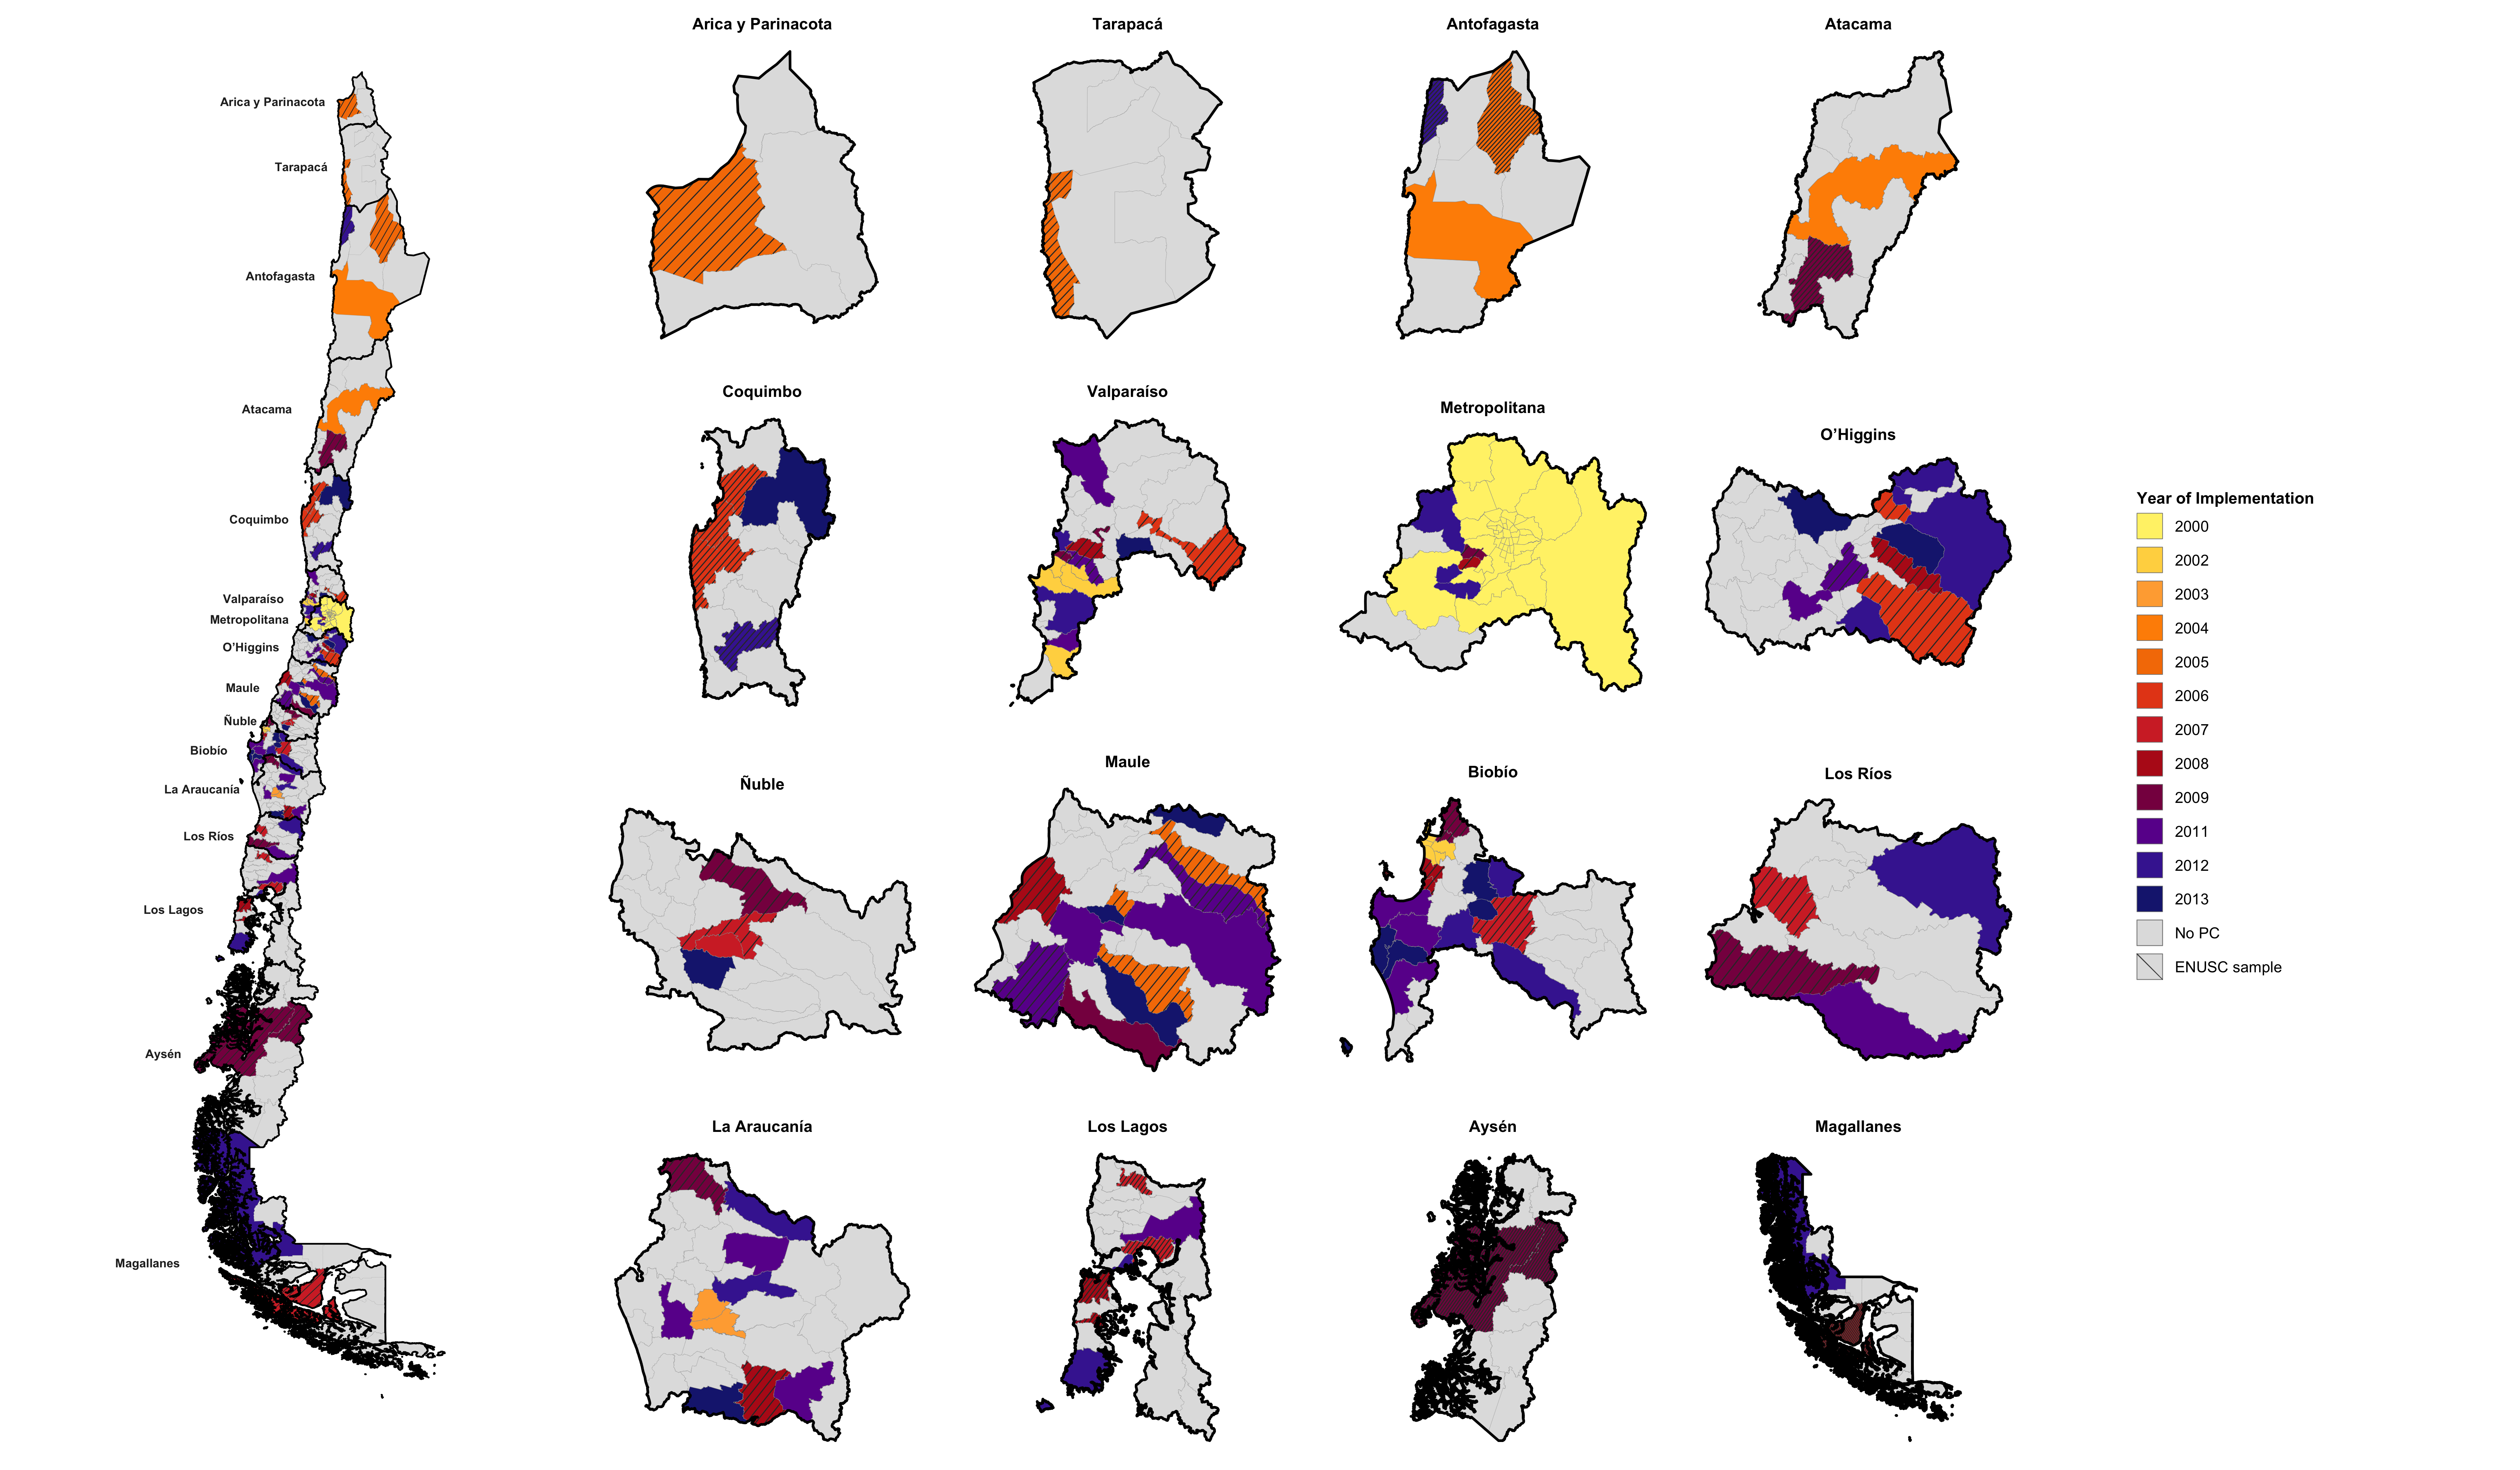
\includegraphics[width=\textwidth]{../manuscript/Graphs/mapa_PCSP_Chile_combinado.png}
    \begin{minipage}{0.95\textwidth}
    \footnotesize
    Notes: This figure shows the spatial rollout of \emph{Plan Cuadrante} across Chilean municipalities. The national map (left) is displayed alongside the 16 regional maps (right) for closer inspection. The color of each treated municipality indicates its year of program adoption, ranging from 2000 (lightest) to 2013 (darkest), following the legend. Municipalities shown in light grey were never treated under PC. Diagonal hatching identifies the 46 treated municipalities in the analytical sample used to estimate the effects on ENUSC outcomes.
    \end{minipage}
\end{figure}
}

\clearpage

{\renewcommand{\thetable}{B.1}
\begin{table}[H]
\caption{Baseline characteristics by subsample}
\label{tab:comparing_samples}
\begin{center}
\resizebox{\textwidth}{!}{
\begin{threeparttable}
\begin{tabular}{l cccccc}
\toprule
&  & \multicolumn{4}{c}{PC municipalities}  & \\
\cmidrule(lr){3-6}
& (1) & (2) & (3) & (4) & (5) & (6) \\
& All & All PC & Always- & Treated & Treated & Never- \\
& municipalities & municipalities & treated & ENUSC & admin.\ data & treated \\
\midrule
Reported crime (per 100k pop.) &     1,650.23 &     2,132.29 &     2,437.25 &     2,202.06 &     1,976.59 &     1,282.47 \\
Arrests (per 100k pop.)        &       267.62     &       442.08     &       606.01     &       459.05     &       358.11     &       134.11     \\
Poverty rate (\%)              &        23.73     &        20.50     &        14.88     &        21.73     &        23.96     &        26.82     \\
Pop.\ density (pop./km$^2$)   &       870.28 &     1,904.14 &     4,593.32 &       215.52 &       134.50 &        27.02 \\
Population                     &    57,857.22         &   117,975.43         &   187,558.74         &   113,079.74         &    81,532.84         &    11,612.44         \\
\midrule
Municipalities                 &          346            &          150            &           58            &           46            &           96            &          196            \\
\bottomrule
\end{tabular}
\begin{tablenotes}[flushleft]
\footnotesize{\item Note: Reported crime, poverty rate, population density, and population are measured as of 2003; arrests are measured as of 2005, the first year for which arrest data are available. Column (1) includes all municipalities in Chile. Column (2) includes all PC municipalities. Column (3) restricts to municipalities that adopted \emph{Plan Cuadrante} before 2005, the always-treated in our sample, which are therefore excluded from our estimation samples (as depicted in Figure 1, panel (a)). Column (4) restricts to treated municipalities in the analytical sample using the ENUSC data. Column (5) restricts to treated municipalities included in the analytical sample using the administrative data. Column (6) includes never-treated municipalities.}
\end{tablenotes}
\end{threeparttable}}
\end{center}
\end{table}
}

\clearpage

{\renewcommand{\thefigure}{C.8}
\begin{figure}[h!]
    \centering
    \caption{Effects of \emph{Plan Cuadrante} on Reported Crime and Arrests Using the Full Set of Post-treatment and Pre-treatment Periods}
    \label{fig:admin_uncapped}
    \begin{subfigure}{0.495\textwidth}
        \centering
        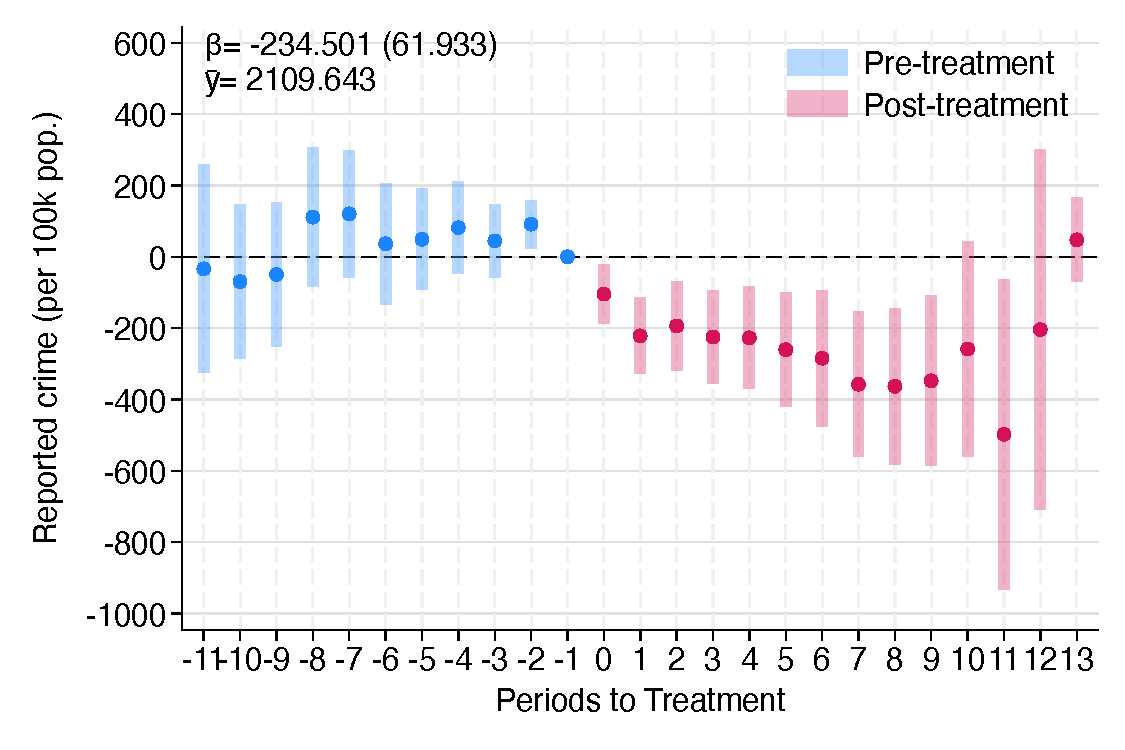
\includegraphics[width=0.98\textwidth]{../manuscript/Graphs/totalreportedcrime_allcomunas_uncapped.pdf}
        \caption{Reported crime per 100k inhabitants}
    \end{subfigure}%
    ~
    \begin{subfigure}{0.495\textwidth}
    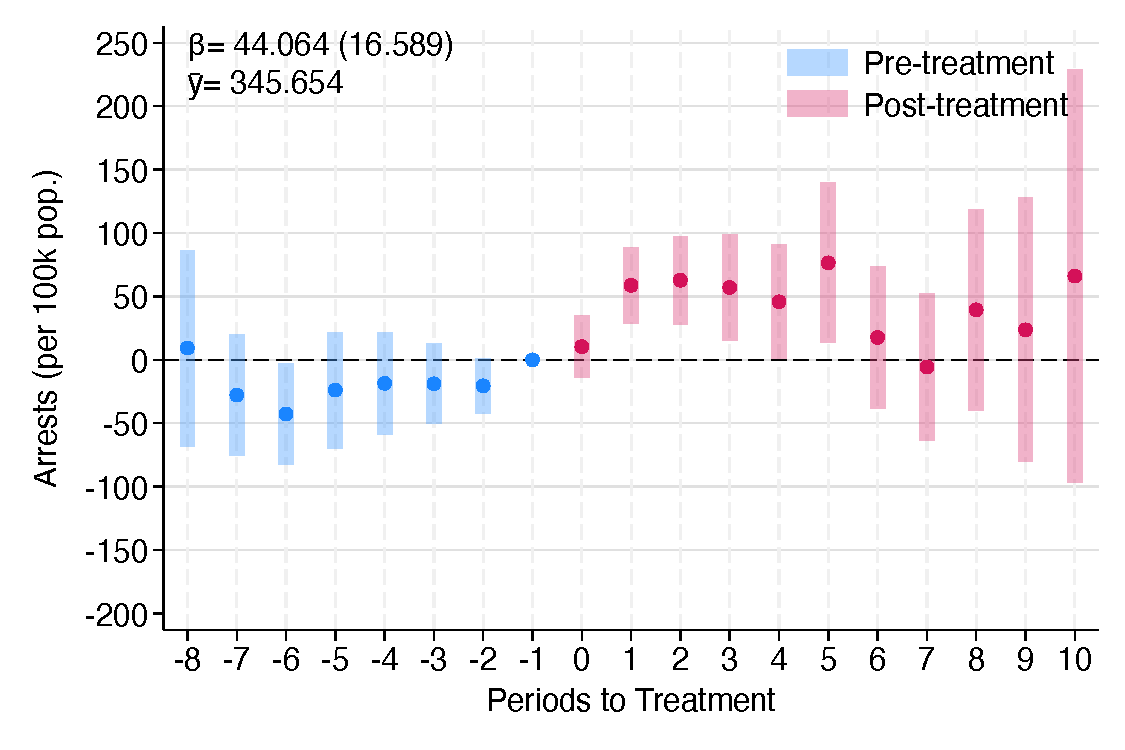
\includegraphics[width=0.98\textwidth]{../manuscript/Graphs/totalarrestscrime_allcomunas_uncapped.pdf}
        \caption{Arrests per 100k inhabitants}
    \end{subfigure}
    \begin{minipage}{\textwidth}
    \footnotesize
   Notes: This figure shows the dynamic effects of \emph{Plan Cuadrante} on the number of crimes reported to the police in the municipality per 100,000 inhabitants (panel a) and on the number of arrests in the municipality per 100,000 inhabitants (panel b), using administrative data. The estimation is conducted using the procedure developed in \citet{Callaway} for difference-in-differences with staggered treatment adoption. The dots in the figure represent the estimated coefficients and the bars behind them 95\% confidence intervals. Standard errors are clustered at the municipality level using the wild bootstrapping procedure. The pooled effect and the mean outcome before the introduction of the treatment are also presented in each panel. Unlike Figure \ref{fig:figure02} in the main text, we do not cap the event study to the same 5 pre-treatment and 6 post-treatment periods used for symmetry with the ENUSC-based analysis. Instead, we exploit the full set of post-treatment and pre-treatment periods. Panel (a) includes 4,371 observations and panel (b) 3,372 observations.
    \end{minipage}
\end{figure}
}

\clearpage

{\renewcommand{\thefigure}{C.7}
\begin{figure}[h!]
    \centering
    \caption{Effects of \emph{Plan Cuadrante} Using a Balanced Panel of Municipalities}
    \label{fig:figureA6_bp}
    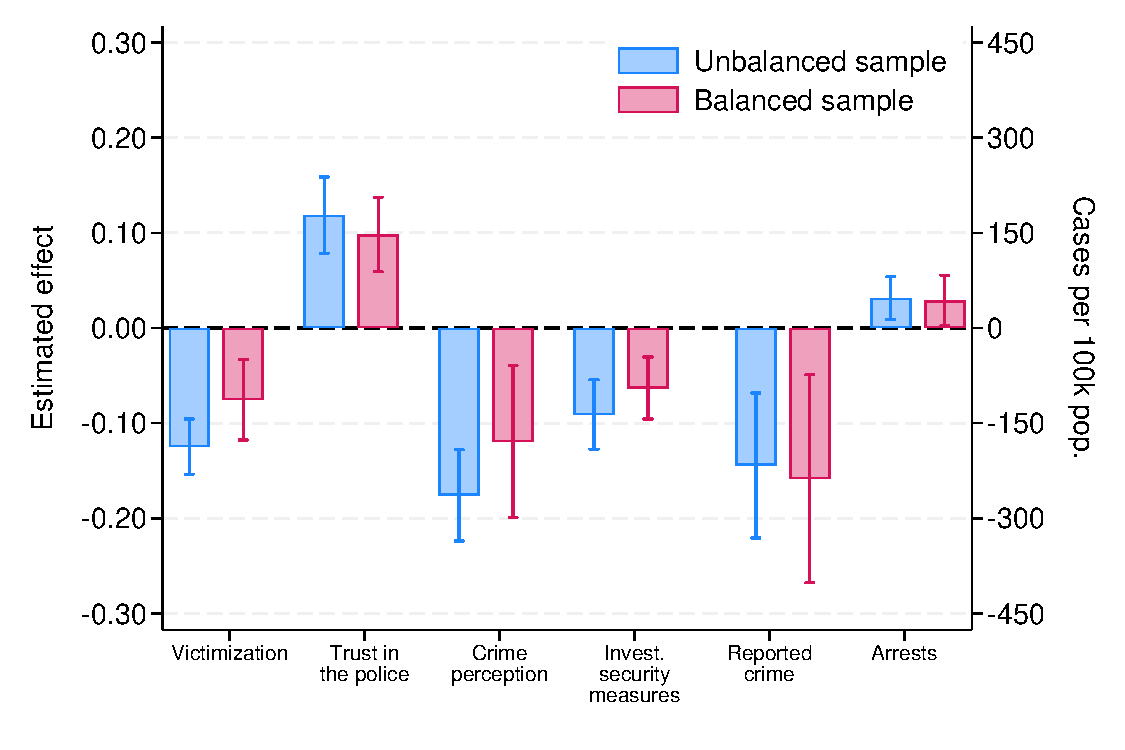
\includegraphics[width=0.8\textwidth]{../manuscript/Graphs/results_crime_balanced_combined.pdf}
    \\[10pt]
    \begin{minipage}{0.99\textwidth}
    \footnotesize Notes: The figure reports the effects of \emph{Plan Cuadrante} on different measures of police effectiveness using the main analytical sample (unbalanced, blue bars) and a balanced panel of municipalities observed over the full event-study window from $t-2$ to $t+3$ (red bars). For the ENUSC sample the balanced panel consists of the 31 municipalities that implemented \emph{Plan Cuadrante} between 2006 and 2009; for the administrative municipality-level sample it consists of 94 municipalities for reported crime and 78 municipalities for arrests. The bars represent the average post-treatment effect estimated with the difference-in-differences estimator developed in \citet{Callaway}, and the whiskers the 95\% confidence intervals; standard errors are clustered at the municipality level. Victimization is the probability of household victimization in the last 12 months; reported crime is the number of crimes reported to the police in the municipality per 100,000 inhabitants; arrests is the number of arrests per 100,000 inhabitants; trust in the police is the probability of reporting high trust in the police; crime perception is the probability of perceiving an increase in crime; and investment in security measures is the probability of adopting security measures in the last twelve months. Reported crime and arrests (administrative data) are read on the right axis; all other outcomes, from the ENUSC survey, are read on the left axis.
    \end{minipage}
\end{figure}
}

\clearpage


\end{response}
\stepcounter{AnsweredComments}




% Comment R2 - 9
\begin{refcomment}

3. Although I appreciate the robustness check to the various difference-in-differences estimators presented in Appendix B, it would be more reassuring to see the event studies.

\label{pt:r2_09}
\end{refcomment}

\begin{response}
    %3. Although I appreciate the robustness check to the various difference-in-differences estimators presented in Appendix B, it would be more reassuring to see the event studies.

Thank you very much for the suggestion. In the revised manuscript, we have expanded the ``Alternative Estimation Methods'' subsection of Appendix \ref{sec:appendixC} to include event-study plots for all main outcomes under each alternative estimator. We have also added a sentence in the Empirical Strategy section noting that the event studies using these staggered difference-in-differences estimators confirm flat pre-adoption trends under all estimation methods.

We reproduce this sentence from the Empirical Strategy section below:

\begin{adjustwidth}{2em}{0em}
Online Appendix Figure \ref{fig:figureA2_alterestim} shows robustness to alternative estimators, including those developed by \citet{Chaisemartin, Gardner, wooldridge2023simple}, as well as to the canonical two-way fixed effects (TWFE) estimator. The resulting estimates are remarkably similar across the alternative staggered-adoption estimators, except for the canonical TWFE, which shows attenuated effects, arguably driven by the negative weights problem discussed above \citep{GoodmanBacon}. The corresponding event studies, reported in Online Appendix Figures \ref{fig:alterestim_delitos}, \ref{fig:alterestim_inseguridad}, \ref{fig:alterestim_medidas}, and \ref{fig:alterestim_crime}, confirm that pre-adoption trends are flat under each alternative estimator.
\end{adjustwidth}

We also reproduce below the expanded ``Alternative Estimation Methods'' subsection of Online Appendix C:

\begin{adjustwidth}{2em}{0em}
The results reported in Section \ref{main_results} are estimated using the difference-in-differences estimator for staggered treatment adoption developed in \citet{Callaway}. In this subsection, we examine the robustness of the results to the use of alternative difference-in-difference estimators for staggered treatment adoption including those developed in \citet{Chaisemartin}, \citet{Gardner}, \citet{wooldridge2023simple}, and also to the canonical two-way fixed effects (TWFE).

The results of these analyses are reported in Figure \ref{fig:figureA2_alterestim} and show similar effects of \emph{Plan Cuadrante} in terms of both magnitude and statistical significance across most specifications. On the other hand, the canonical TWFE shows smaller effects, likely due to the negative weights problem highlighted by \citet{GoodmanBacon} when estimating difference-in-differences with staggered treatment adoption using TWFE.

Figures \ref{fig:alterestim_delitos} through \ref{fig:alterestim_crime} report the corresponding event-study estimates for victimization, crime perception, investment in security measures, and reported crime under each alternative estimator. Pre-treatment coefficients are consistently small and statistically indistinguishable from zero across all estimators and outcomes, confirming that the parallel trends assumption holds regardless of the estimation method. Post-treatment effects remain negative and statistically significant across these outcomes, closely mirroring the results from the main specification in Figure \ref{fig:figure02}.
\end{adjustwidth}

\clearpage
\noindent\textbf{Other figures referenced above:}
\vspace{0.5em}

{\renewcommand{\thefigure}{C.2}
\begin{figure}[h!]
    \centering
    \caption[Effects of \emph{Plan Cuadrante} on Police Effectiveness Using Alternative Estimators]{Effects of \emph{Plan Cuadrante} on Police Effectiveness Using Alternative Estimators}
    \label{fig:figureA2_alterestim}
    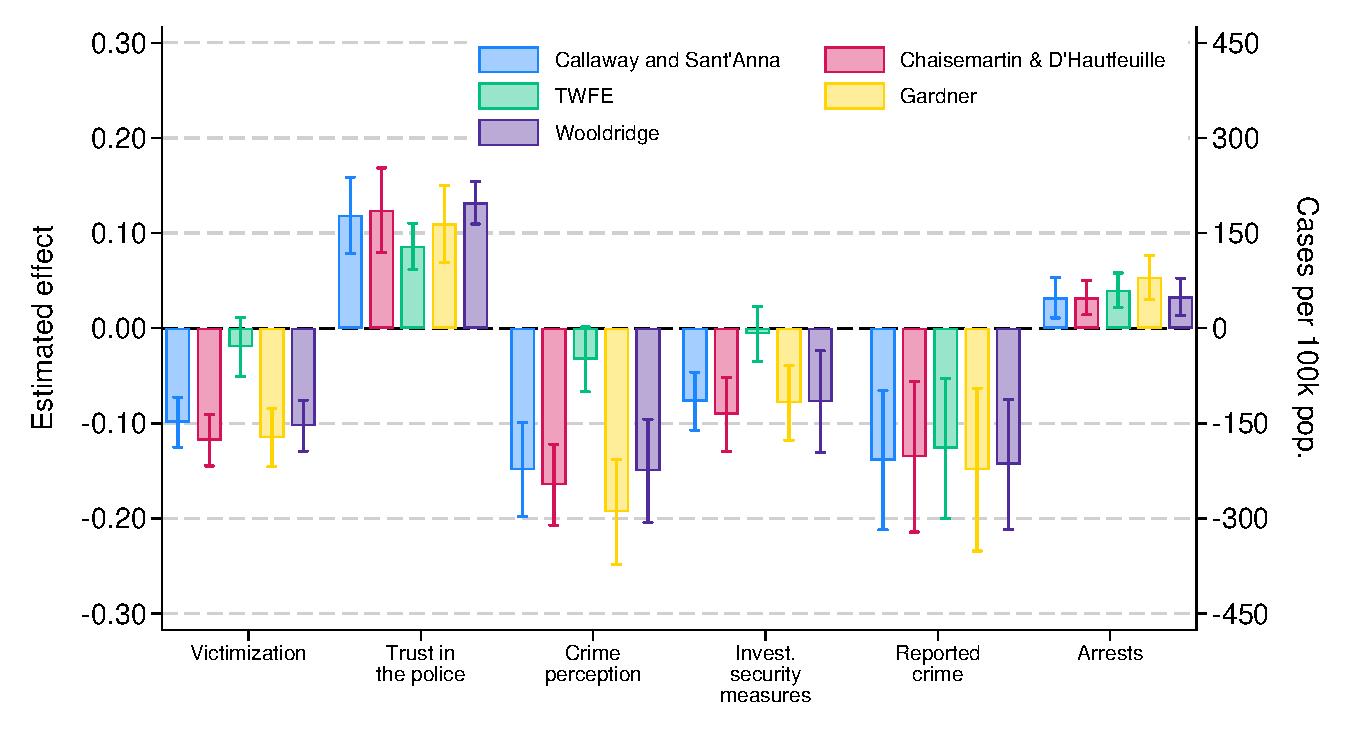
\includegraphics[width=\textwidth]{../manuscript/Graphs/Comparison_estimators_combined.pdf}
    \\[8pt]
    \begin{minipage}{0.99\textwidth}
    \footnotesize Notes: The figure reports the effects of \emph{Plan Cuadrante} on different measures of police effectiveness using various difference-in-differences estimators, including the methods developed in \citet{Callaway}, \citet{Chaisemartin}, \citet{Gardner}, \citet{wooldridge2023simple}, and the canonical two-way fixed effects (TWFE). Bars are the estimated post-treatment effects and the whiskers the 95\% confidence intervals; standard errors are clustered at the municipality level. Victimization is the probability of household victimization in the last 12 months; reported crime is the number of crimes reported to the police in the municipality per 100,000 inhabitants; crime perception is the probability of perceiving an increase in crime; investment in security measures is the probability of adopting security measures in the last twelve months; trust in the police is the probability of reporting high trust in the police; and arrests is the number of arrests per 100,000 inhabitants. Reported crime and arrests (administrative data) are read on the right axis; all other outcomes, from the ENUSC survey, are read on the left axis.
    \end{minipage}
\end{figure}
}

\clearpage

{\setcounter{figure}{2}\renewcommand{\thefigure}{C.\arabic{figure}}
% =============================================================================
% Alternative-estimator robustness figures
% Each figure shows the event study from three estimators:
%   (a) Chaisemartin & D'Hautfeuille
%   (b) Gardner
%   (c) Wooldridge
% Callaway & Sant'Anna is excluded — it appears as the headline figure.
%
% First block (3 figures): ENUSC survey outcomes
% Second block (1 figure): SPD administrative crime outcomes
% =============================================================================


% ----- Victimization (delitos) -----------------------------------------------
\begin{figure}[h!]
    \centering
    \caption[Effects of \emph{Plan Cuadrante} on Victimization Using Alternative Estimators]{Effects of \emph{Plan Cuadrante} on Victimization Using Alternative Estimators}
    \label{fig:alterestim_delitos}
    \begin{subfigure}{0.47\textwidth}
        \centering
        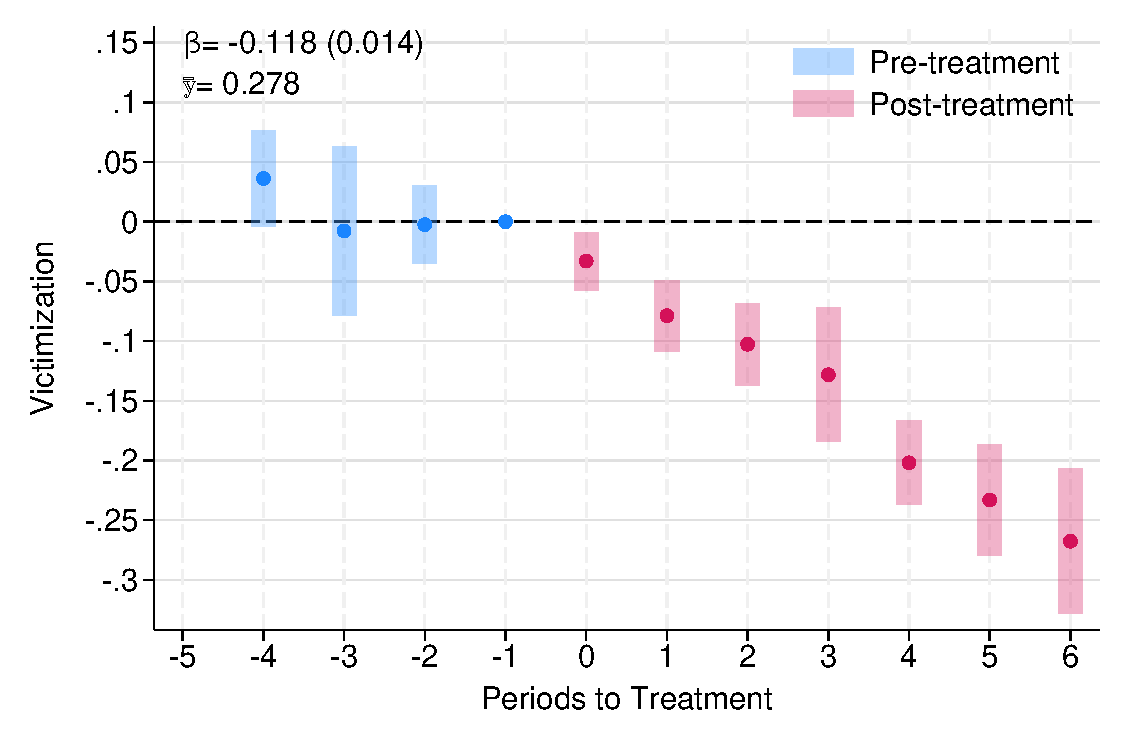
\includegraphics[width=\textwidth]{../manuscript/Graphs/CHDH_event_study_delitos.pdf}
        \caption{Chaisemartin \& D'Hautfeuille}
    \end{subfigure}%
    \begin{subfigure}{0.47\textwidth}
        \centering
        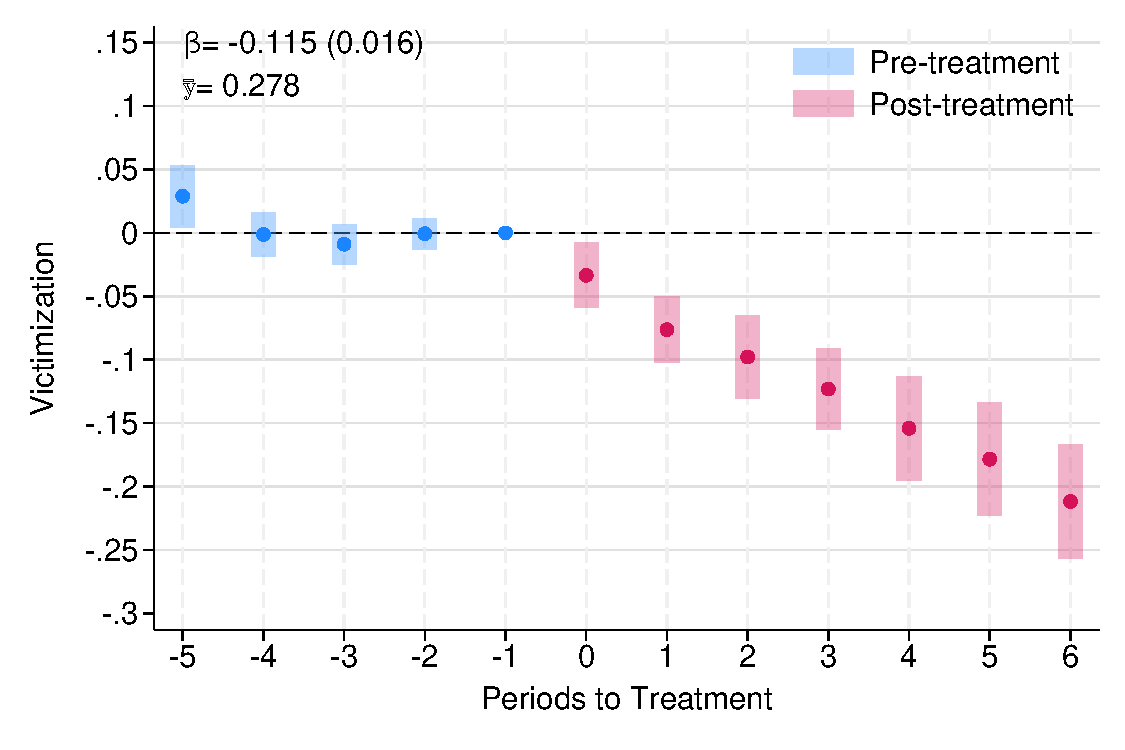
\includegraphics[width=\textwidth]{../manuscript/Graphs/DID2S_event_study_delitos.pdf}
        \caption{Gardner}
    \end{subfigure}
    \\[6pt]
    \begin{subfigure}{0.47\textwidth}
        \centering
        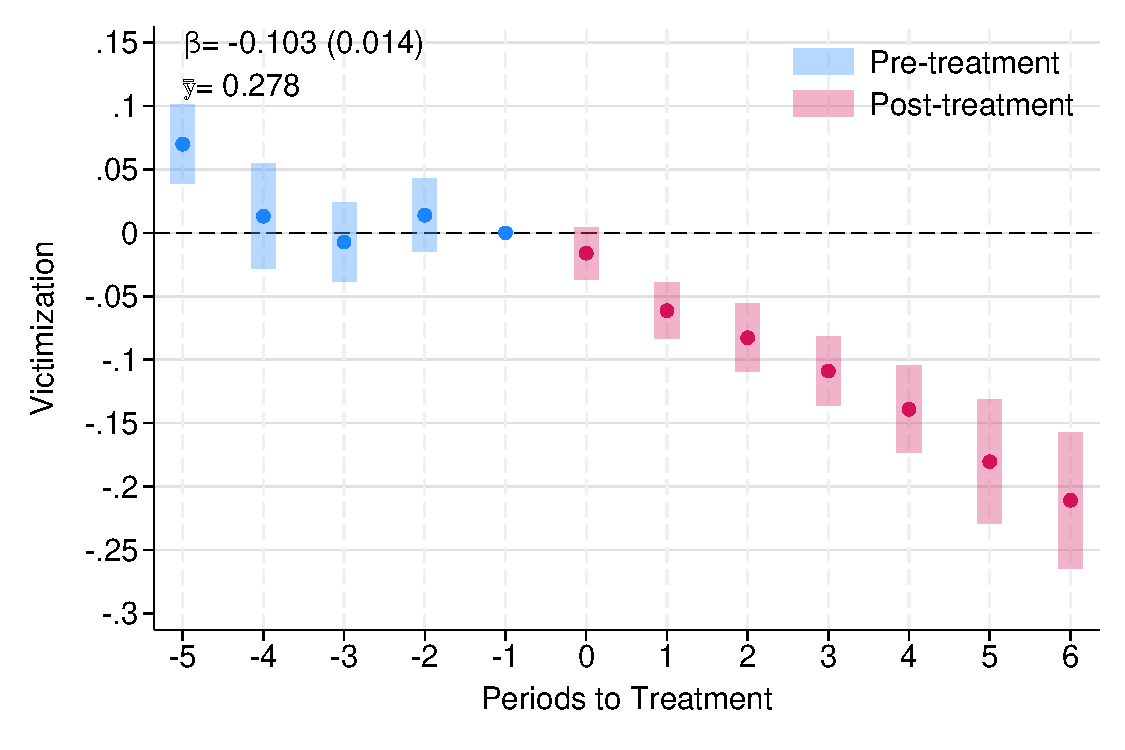
\includegraphics[width=\textwidth]{../manuscript/Graphs/JWDID_event_study_delitos.pdf}
        \caption{Wooldridge}
    \end{subfigure}
    \\[12pt]
    \begin{minipage}{0.99\textwidth}
    \footnotesize Notes: The figure reports event-study estimates of the effect of \emph{Plan Cuadrante} on the probability of household victimization in the last 12 months using the ENUSC survey, estimated with three alternative difference-in-differences estimators robust to staggered adoption: \citet{Chaisemartin} in panel (a), \citet{Gardner} in panel (b), and \citet{wooldridge2023simple} in panel (c). Each panel plots the estimated coefficient at each event time relative to treatment along with 95\% confidence intervals. Standard errors are clustered at the municipality level. The headline coefficient $\beta$ corresponds to the average post-treatment effect, and $\bar{y}$ denotes the never-treated mean of the outcome over the sample period.
    \end{minipage}
\end{figure}


% ----- Crime perception (inseguridad_barrio1) --------------------------------
\begin{figure}[h!]
    \centering
    \caption[Effects of \emph{Plan Cuadrante} on Crime Perception Using Alternative Estimators]{Effects of \emph{Plan Cuadrante} on Crime Perception Using Alternative Estimators}
    \label{fig:alterestim_inseguridad}
    \begin{subfigure}{0.47\textwidth}
        \centering
        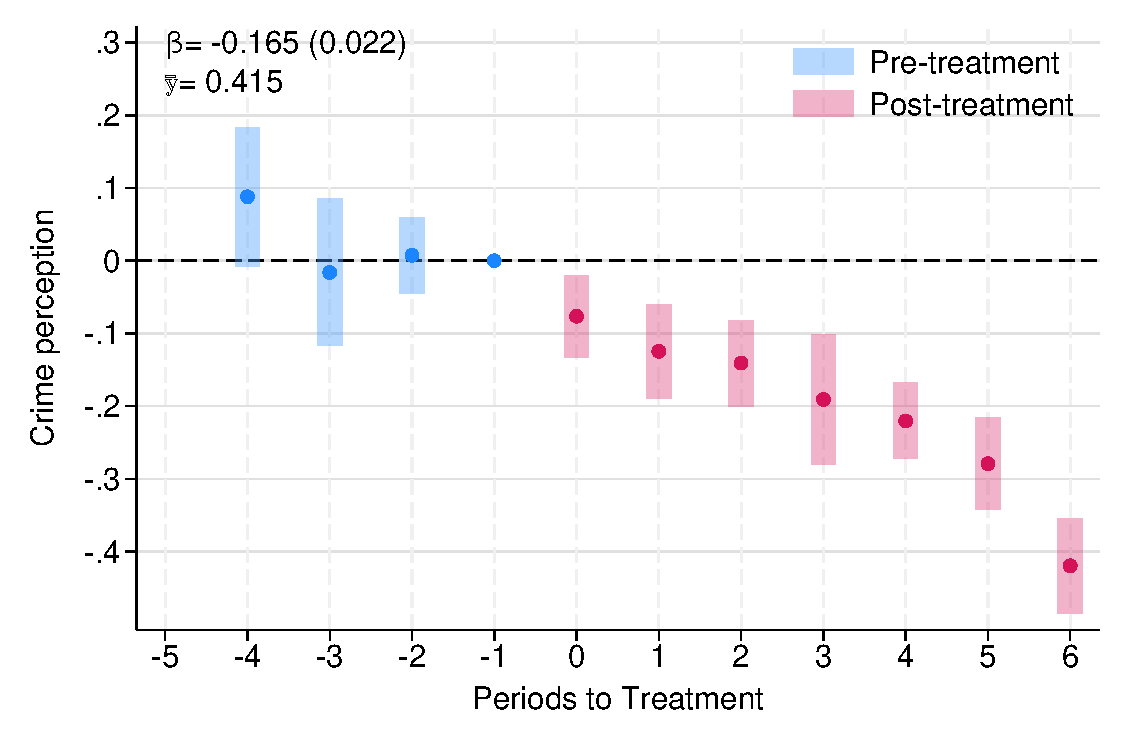
\includegraphics[width=\textwidth]{../manuscript/Graphs/CHDH_event_study_inseguridad_barrio1.pdf}
        \caption{Chaisemartin \& D'Hautfeuille}
    \end{subfigure}%
    \begin{subfigure}{0.47\textwidth}
        \centering
        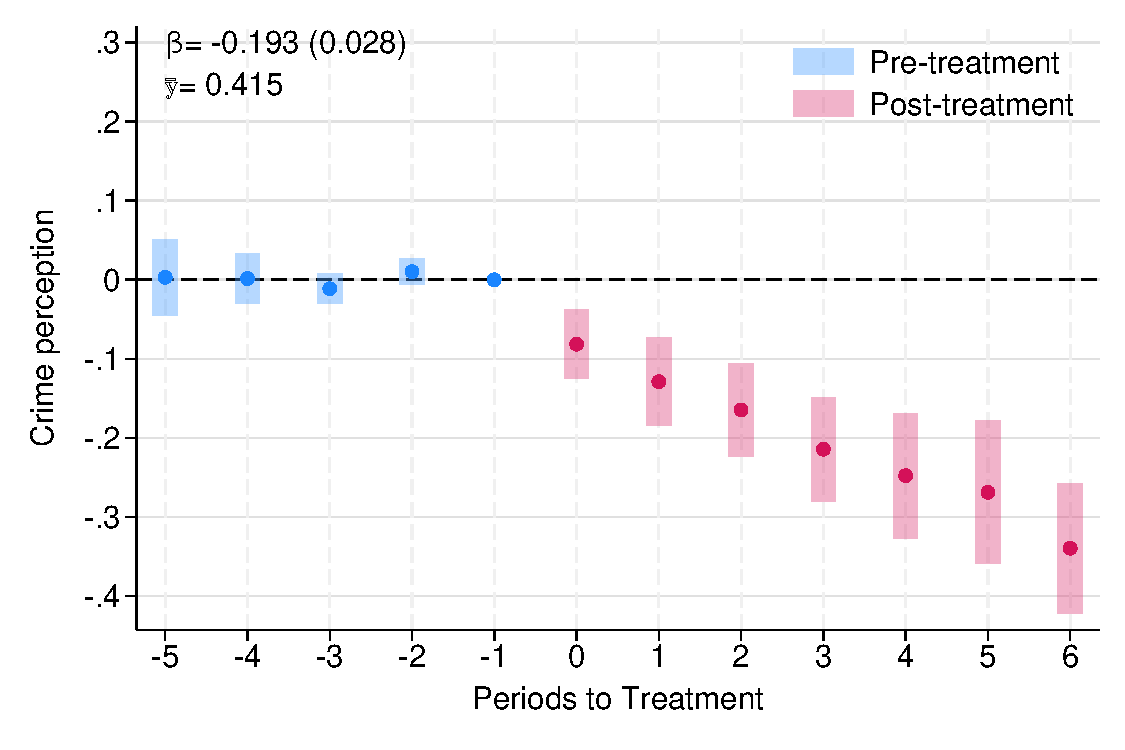
\includegraphics[width=\textwidth]{../manuscript/Graphs/DID2S_event_study_inseguridad_barrio1.pdf}
        \caption{Gardner}
    \end{subfigure}
    \\[6pt]
    \begin{subfigure}{0.47\textwidth}
        \centering
        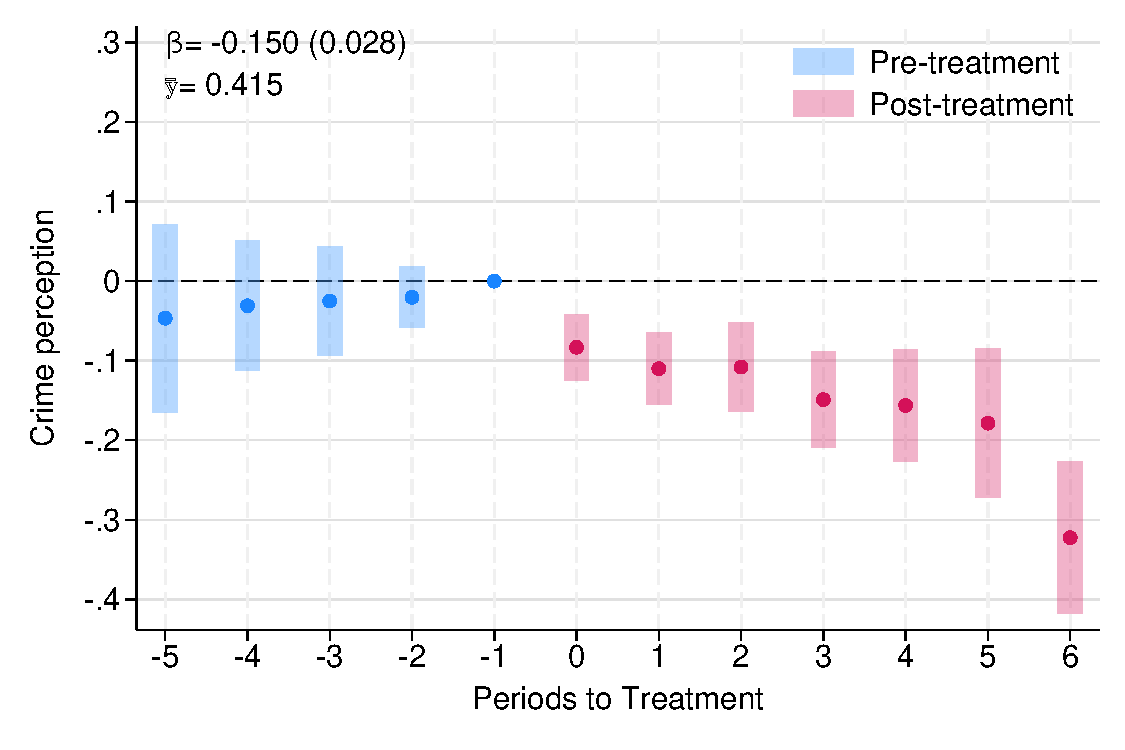
\includegraphics[width=\textwidth]{../manuscript/Graphs/JWDID_event_study_inseguridad_barrio1.pdf}
        \caption{Wooldridge}
    \end{subfigure}
    \\[12pt]
    \begin{minipage}{0.99\textwidth}
    \footnotesize Notes: The figure reports event-study estimates of the effect of \emph{Plan Cuadrante} on the probability of perceiving an increase in crime using the ENUSC survey, estimated with three alternative difference-in-differences estimators robust to staggered adoption: \citet{Chaisemartin} in panel (a), \citet{Gardner} in panel (b), and \citet{wooldridge2023simple} in panel (c). Each panel plots the estimated coefficient at each event time relative to treatment along with 95\% confidence intervals. Standard errors are clustered at the municipality level. The headline coefficient $\beta$ corresponds to the average post-treatment effect, and $\bar{y}$ denotes the never-treated mean of the outcome over the sample period.
    \end{minipage}
\end{figure}


% ----- Private investment in security (medidas_general_12) -------------------
\begin{figure}[h!]
    \centering
    \caption[Effects of \emph{Plan Cuadrante} on Investment in Security Measures Using Alternative Estimators]{Effects of \emph{Plan Cuadrante} on Investment in Security Measures Using Alternative Estimators}
    \label{fig:alterestim_medidas}
    \begin{subfigure}{0.47\textwidth}
        \centering
        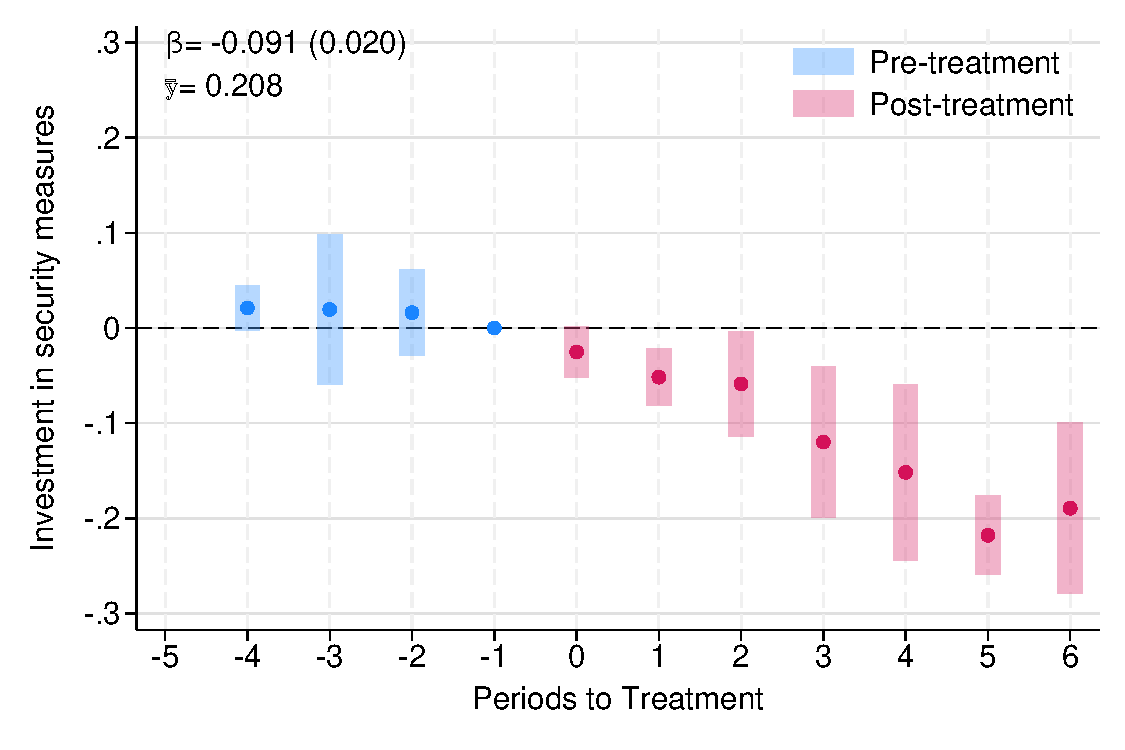
\includegraphics[width=\textwidth]{../manuscript/Graphs/CHDH_event_study_medidas_general_12.pdf}
        \caption{Chaisemartin \& D'Hautfeuille}
    \end{subfigure}%
    \begin{subfigure}{0.47\textwidth}
        \centering
        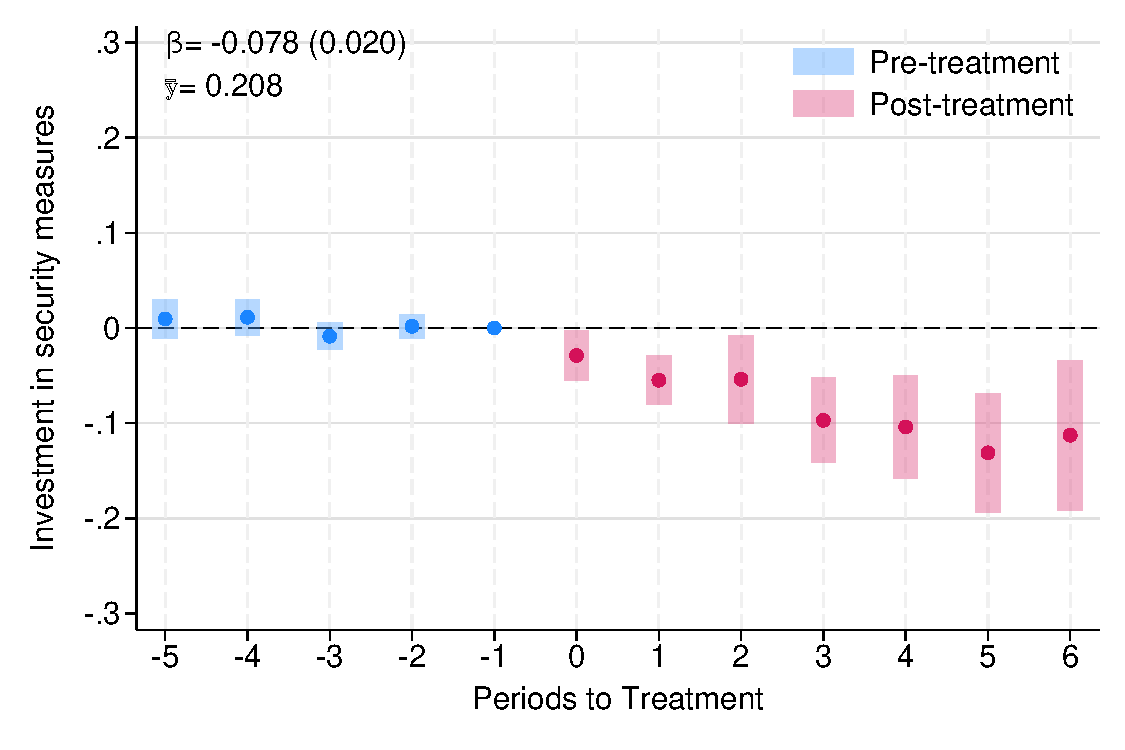
\includegraphics[width=\textwidth]{../manuscript/Graphs/DID2S_event_study_medidas_general_12.pdf}
        \caption{Gardner}
    \end{subfigure}
    \\[6pt]
    \begin{subfigure}{0.47\textwidth}
        \centering
        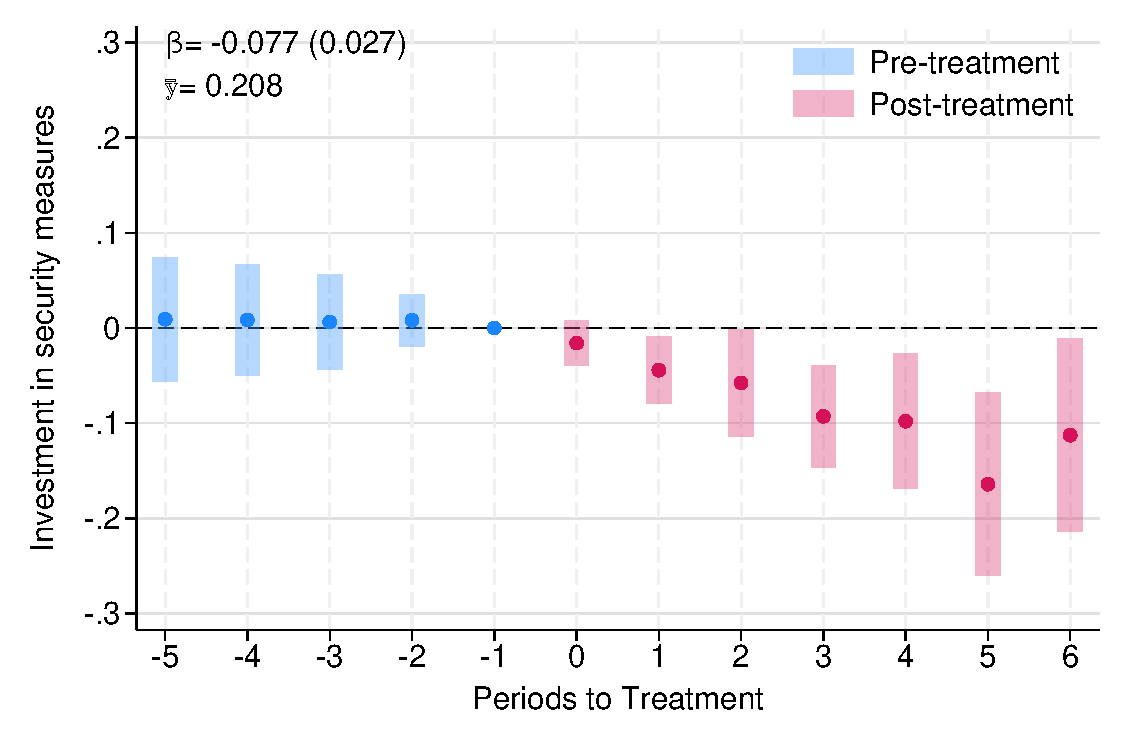
\includegraphics[width=\textwidth]{../manuscript/Graphs/JWDID_event_study_medidas_general_12.pdf}
        \caption{Wooldridge}
    \end{subfigure}
    \\[12pt]
    \begin{minipage}{0.99\textwidth}
    \footnotesize Notes: The figure reports event-study estimates of the effect of \emph{Plan Cuadrante} on the probability of adopting security measures in the last twelve months using the ENUSC survey, estimated with three alternative difference-in-differences estimators robust to staggered adoption: \citet{Chaisemartin} in panel (a), \citet{Gardner} in panel (b), and \citet{wooldridge2023simple} in panel (c). Each panel plots the estimated coefficient at each event time relative to treatment along with 95\% confidence intervals. Standard errors are clustered at the municipality level. The headline coefficient $\beta$ corresponds to the average post-treatment effect, and $\bar{y}$ denotes the never-treated mean of the outcome over the sample period.
    \end{minipage}
\end{figure}


% =============================================================================
% Administrative data (SPD municipality-level)
% =============================================================================


% ----- Reported crime --------------------------------------------------------
\begin{figure}[h!]
    \centering
    \caption[Effects of \emph{Plan Cuadrante} on Reported Crime Using Alternative Estimators]{Effects of \emph{Plan Cuadrante} on Reported Crime Using Alternative Estimators}
    \label{fig:alterestim_crime}
    \begin{subfigure}{0.47\textwidth}
        \centering
        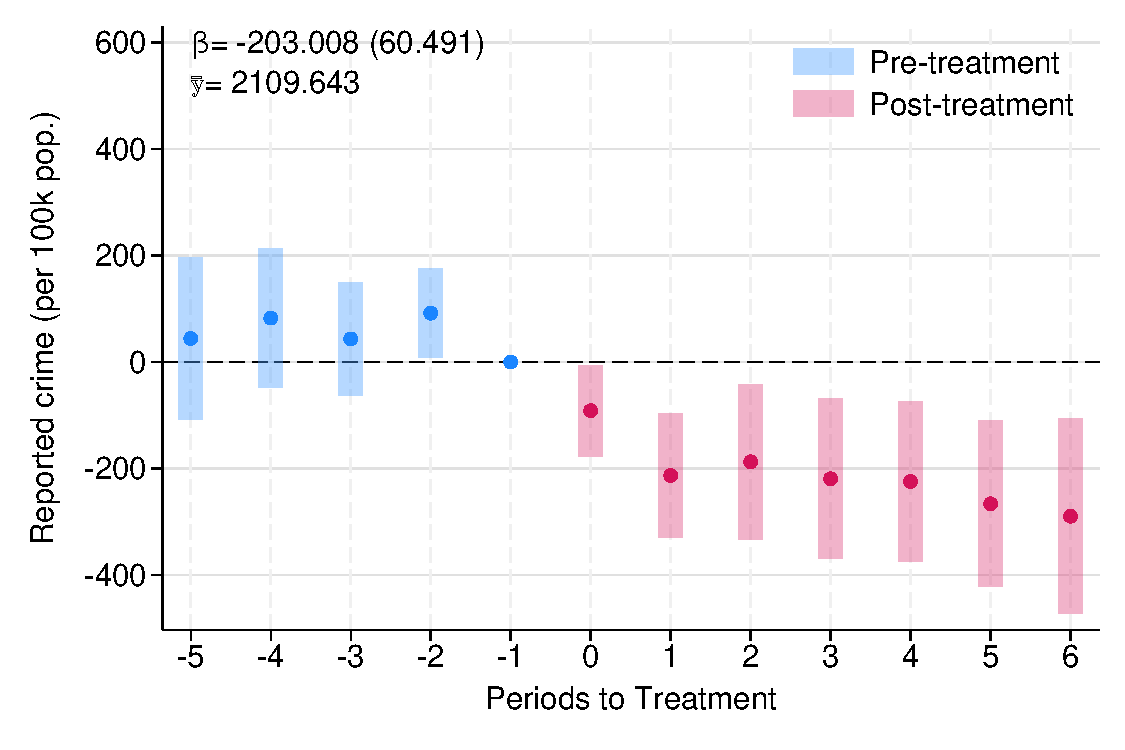
\includegraphics[width=\textwidth]{../manuscript/Graphs/CHDH_event_study_crime.pdf}
        \caption{Chaisemartin \& D'Hautfeuille}
    \end{subfigure}%
    \begin{subfigure}{0.47\textwidth}
        \centering
        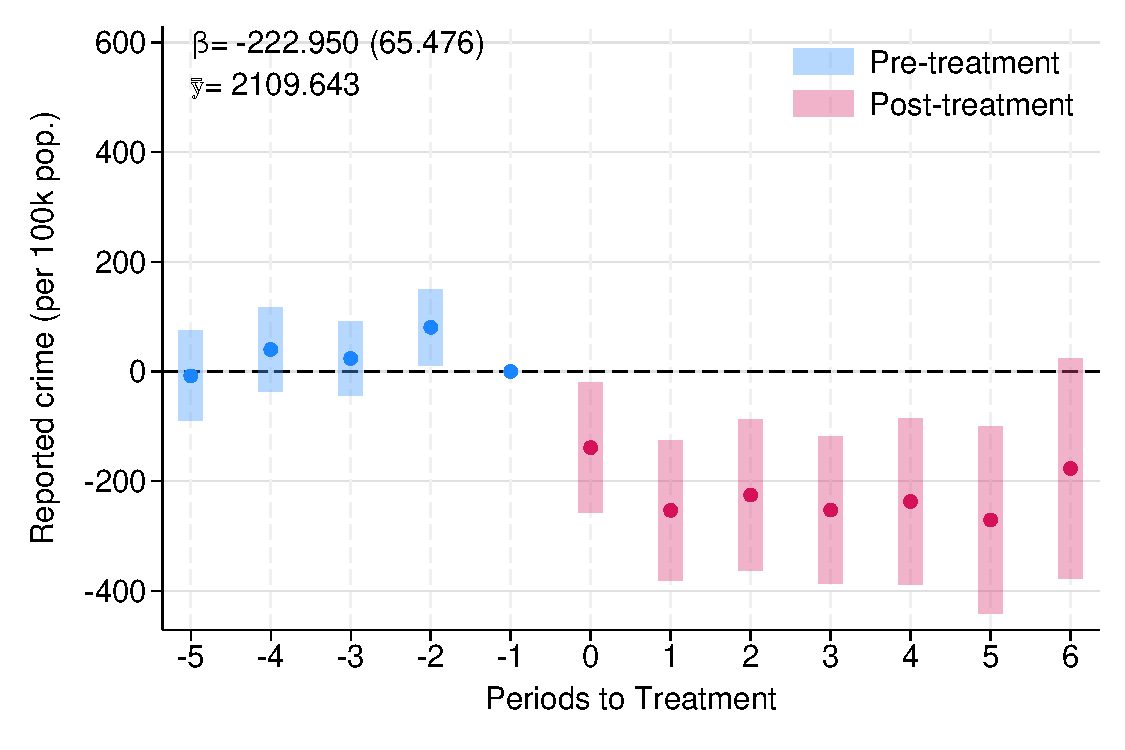
\includegraphics[width=\textwidth]{../manuscript/Graphs/DID2S_event_study_crime.pdf}
        \caption{Gardner}
    \end{subfigure}
    \\[6pt]
    \begin{subfigure}{0.47\textwidth}
        \centering
        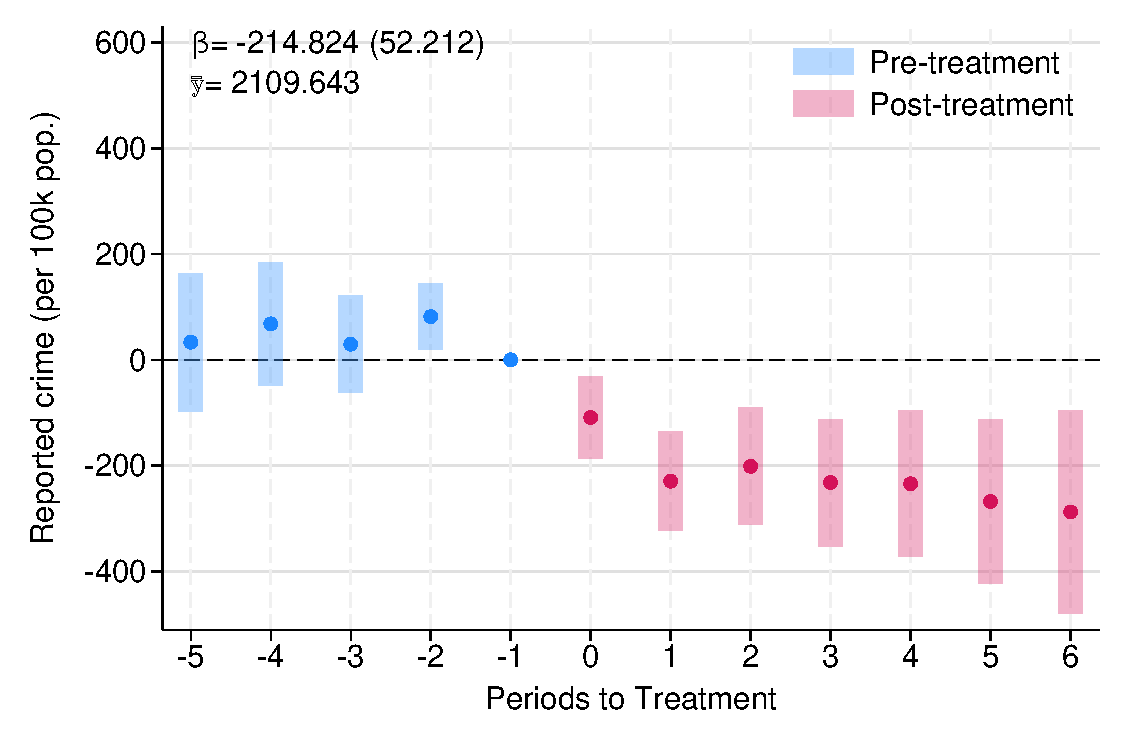
\includegraphics[width=\textwidth]{../manuscript/Graphs/JWDID_event_study_crime.pdf}
        \caption{Wooldridge}
    \end{subfigure}
    \\[12pt]
    \begin{minipage}{0.99\textwidth}
    \footnotesize Notes: The figure reports event-study estimates of the effect of \emph{Plan Cuadrante} on the number of crimes reported to the police in the municipality per 100,000 inhabitants using administrative data, estimated with three alternative difference-in-differences estimators robust to staggered adoption: \citet{Chaisemartin} in panel (a), \citet{Gardner} in panel (b), and \citet{wooldridge2023simple} in panel (c). Each panel plots the estimated coefficient at each event time relative to treatment along with 95\% confidence intervals. Standard errors are clustered at the municipality level. The headline coefficient $\beta$ is the equal-weighted average of the post-treatment effects from $t=0$ to $t=6$, and $\bar{y}$ denotes the never-treated mean of the outcome over the sample period.
    \end{minipage}
\end{figure}
}

\clearpage

\end{response}
\stepcounter{AnsweredComments}

% Comment R2 - 10
\begin{refcomment}

 4. Given the large number of related outcomes (e.g., Figure 2), the authors may want to consider adjustments for multiple hypothesis testing. 

\label{pt:r2_10}
\end{refcomment}

\begin{response}
    %4.	Given the large number of related outcomes (e.g., Figure 2), the authors may want to consider adjustments for multiple hypothesis testing.


We thank the reviewer for this suggestion.

We acknowledge that testing multiple outcomes simultaneously raises concerns about false discoveries. We note, however, that all six outcomes in our main analysis---including the four now presented in Figure 2 and the arrests and trust-in-police outcomes moved to the mechanisms section in the revised manuscript---are statistically significant at the 1\% significance level. Under the null hypothesis of no effects, one would expect at most 1\% of tested coefficients to be false positives by chance at the same level. The observed pattern of results is therefore difficult to reconcile with false discoveries driven by multiple testing. Nonetheless, to address this concern formally, we apply a multiple hypothesis testing correction to the p-values. While procedures such as \citet{romano2005} would be the natural choice, their implementation is not computationally straightforward with the \citet{Callaway} estimator. We therefore apply the Bonferroni correction, which can be applied directly to any set of estimated p-values regardless of the underlying estimator. The adjusted p-values, reported in Table \ref{tab:bonferroni}, confirm that the main results remain statistically significant after correction for every outcome considered. 

In the revised manuscript, we have added the following footnote in Section 4.1: 


\begin{adjustwidth}{2em}{0em}
Table \ref{tab:bonferroni} in Online Appendix \ref{sec:appendixC} applies the Bonferroni correction across the main outcome estimates and confirms that these results are not a product of multiple hypothesis testing.
\end{adjustwidth}

We also add the following subsection, ``Multiple Hypothesis Testing,'' to Online Appendix C reporting this exercise in detail:

\begin{adjustwidth}{2em}{0em}
Testing multiple outcomes simultaneously raises concerns about false discoveries. In our analyses, all six outcomes in our main analyses are statistically significant at the 1\% significance level. Under the null hypothesis of no effects, one would expect at most 1\% of tested coefficients to be false positives by chance at the same level. The observed pattern of results is therefore difficult to reconcile with false discoveries driven by multiple testing. Nonetheless, to address this concern formally, we apply a multiple hypothesis testing correction to the p-values. While procedures such as \citet{romano2005} would be a natural choice, their implementation is not computationally straightforward with the \citet{Callaway} estimator. We therefore apply the Bonferroni correction, which can be applied directly to any set of estimated p-values regardless of the underlying estimator. The adjusted p-values, reported in Table \ref{tab:bonferroni}, confirm that the main results remain statistically significant at conventional confidence levels after correction for every outcome considered.
\end{adjustwidth}

\clearpage
\noindent\textbf{Other figure and table referenced above:}
\vspace{0.5em}

{\setcounter{figure}{1}\renewcommand{\thefigure}{\arabic{figure}}
%--- Implementation
\begin{figure}[h!]
    \centering
    \caption{Effects of \emph{Plan Cuadrante} on Crime Outcomes and Security Perceptions}
    \label{fig:figure02}
    \begin{subfigure}{0.495\textwidth}
        \centering
        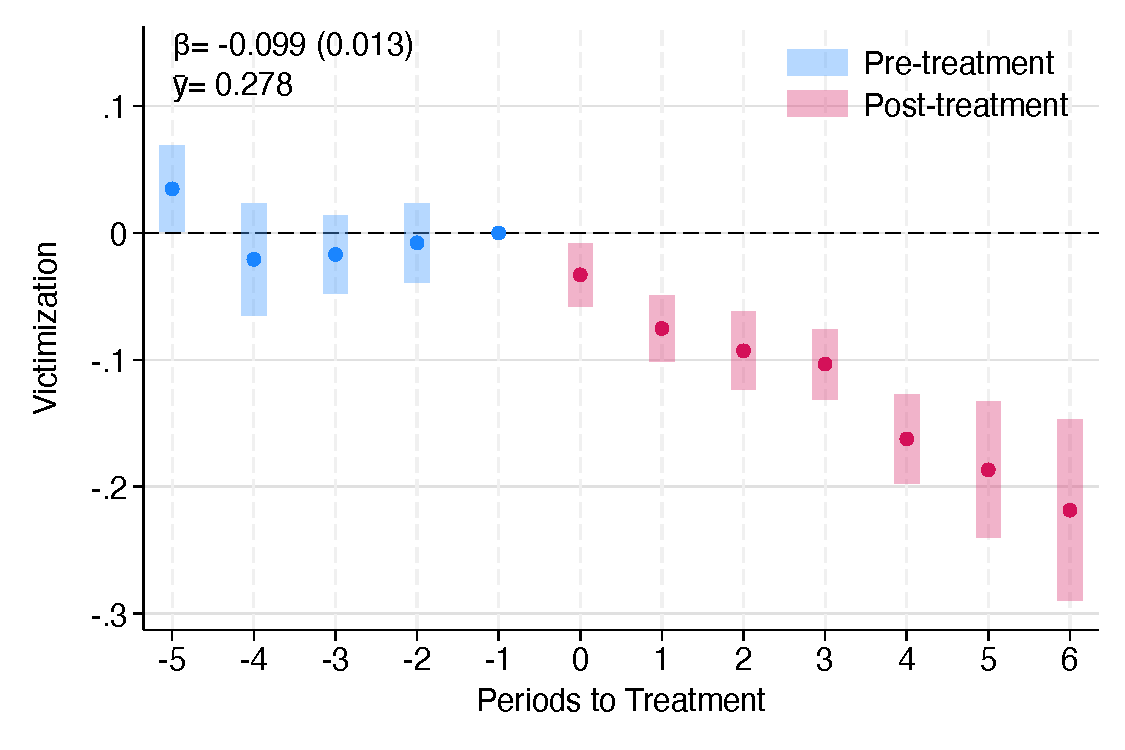
\includegraphics[width=\textwidth]{../manuscript/Graphs/results_victimization.pdf}
        \caption{Victimization in last 12 months}
    \end{subfigure}%
    ~
    \begin{subfigure}{0.495\textwidth}
    \centering
    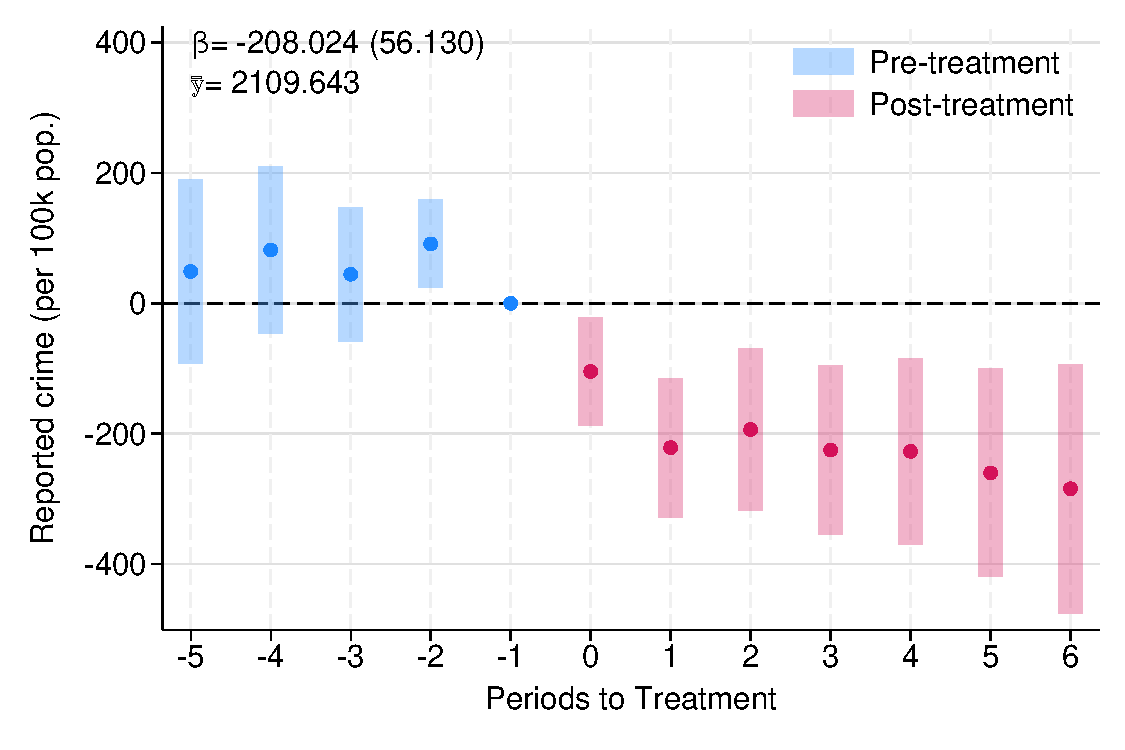
\includegraphics[width=\textwidth]{../manuscript/Graphs/totalreportedcrime_allcomunas.pdf}
        \caption{Reported crime per 100k inhabitants}
    \end{subfigure}
        \begin{subfigure}{0.495\textwidth}
        \centering
        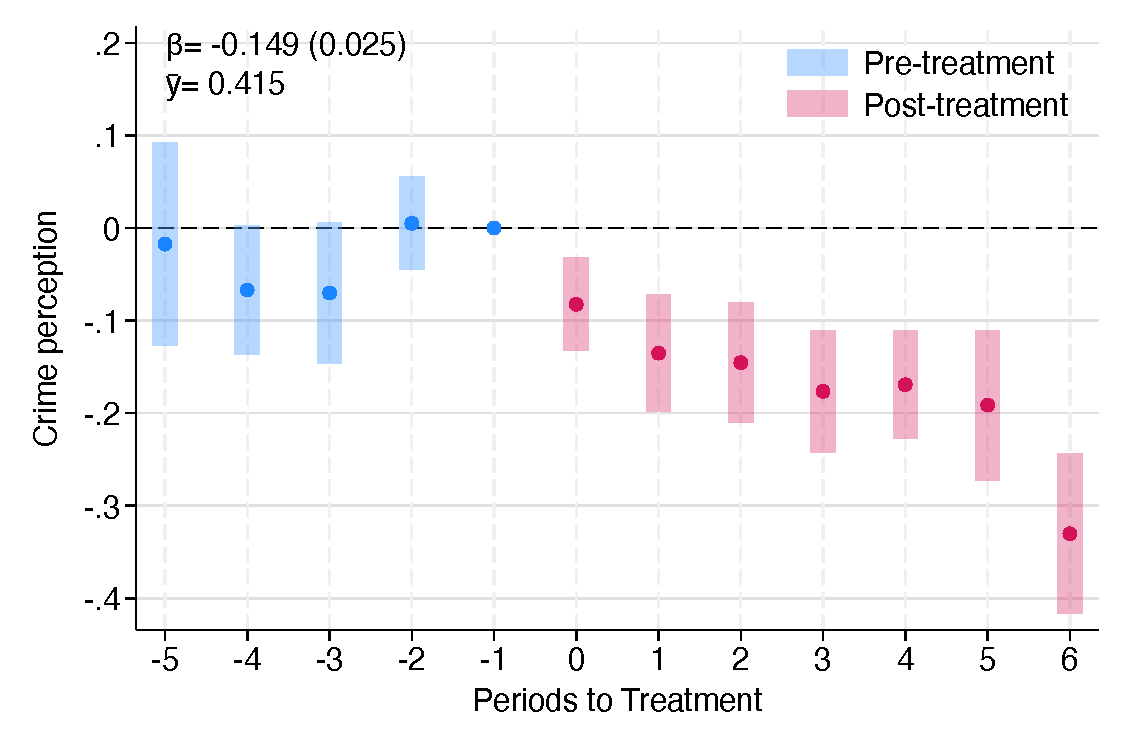
\includegraphics[width=\textwidth]{../manuscript/Graphs/results_perception.pdf}
        \caption{Households reporting an increase in crime}
    \end{subfigure}%
    ~
    \begin{subfigure}{0.495\textwidth}
    \centering
    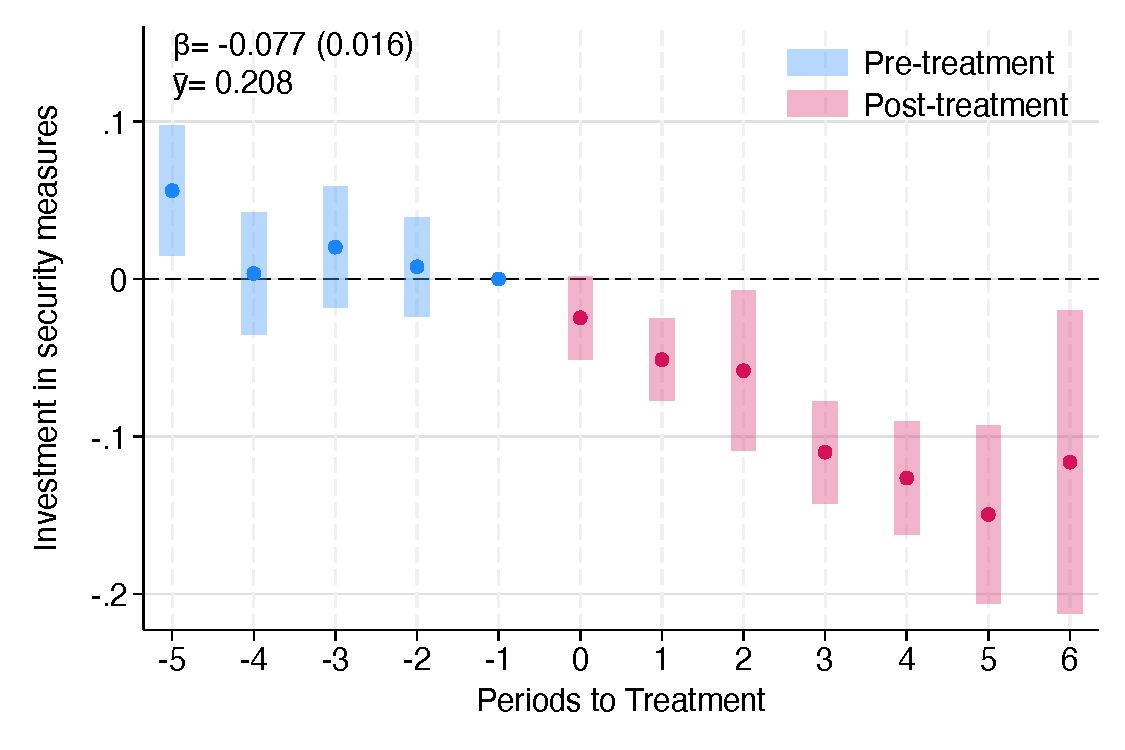
\includegraphics[width=\textwidth]{../manuscript/Graphs/results_hhprotectionmeasures.pdf}
        \caption{Households adopting security measures}
    \end{subfigure}
    \\[12pt]
    \begin{minipage}{0.99\textwidth}
    \footnotesize
    Notes: This figure shows the dynamic effects of the \emph{Plan Cuadrante} on different measures of police effectiveness. The estimation is conducted using the procedure developed in \citet{Callaway} for difference-in-differences with staggered treatment adoption. The dots in the figure represent the estimated coefficients and the bars behind them 95\% confidence intervals. Standard errors are clustered at the municipality level using the wild bootstrapping procedure. The pooled effect and the mean outcome before the introduction of the treatment is also presented in each panel. Panel (a) reports the effect of \emph{Plan Cuadrante} on the probability of household victimization in the last 12 months using the ENUSC survey. Panel (b) reports the effect on the number of crimes reported to the police in the municipality per 100,000 inhabitants using administrative data. Panel (c) reports the effect on the probability of perceiving an increase in crime using the ENUSC survey. Panel (d) reports the effect on the probability of adopting security measures in the last twelve months using the ENUSC survey. Panel (a) includes 93,041 observations; panel (b), 4,231; panel (c), 89,578; and panel (d), 93,041 observations.
    \end{minipage}
\end{figure}
}

\clearpage

{\renewcommand{\thetable}{C.2}
\begin{table}[H]
\centering
\caption{Multiple Hypothesis Testing: Bonferroni Correction}
\label{tab:bonferroni}
\begin{tabular}{lcccc}
\toprule
Outcome & \multicolumn{2}{c}{} & \multicolumn{2}{c}{Bonferroni} \\
 & \multicolumn{2}{c}{Original} & \multicolumn{2}{c}{adjusted} \\
\cmidrule(lr){2-3} \cmidrule(lr){4-5}
 & p-value & & p-value & \\
\midrule
Victimization & 0.00000 & *** & 0.00000 & *** \\
Reported crime (per 100k pop.) & 0.00021 & *** & 0.00126 & *** \\
Crime perception & 0.00000 & *** & 0.00000 & *** \\
Investment in security measures & 0.00000 & *** & 0.00000 & *** \\
Trust in the police & 0.00000 & *** & 0.00000 & *** \\
Arrests (per 100k pop.) & 0.00316 & *** & 0.01896 & ** \\
\midrule
\multicolumn{5}{l}{\footnotesize Notes: Bonferroni correction multiplies each p-value by the number of} \\
\multicolumn{5}{l}{\footnotesize outcomes tested ($n=6$). Significance levels: *** $p<0.01$, ** $p<0.05$, * $p<0.1$.}
\end{tabular}
\end{table}}

\clearpage



\end{response}
\stepcounter{AnsweredComments}



% Comment R2 - 11
\begin{refcomment}

 5. I would qualify the claims associated to Table B1 since column (2) shows an estimate twice as large as that in column (1), and column (4) does not allow to reject an ATT equal to zero.

\label{pt:r2_11}
\end{refcomment}

\begin{response}
    % 5.	I would qualify the claims associated to Table B1 since column (2) shows an estimate twice as large as that in column (1), and column (4) does not allow to reject an ATT equal to zero.

Thanks for the point. We agree that the description of the results of this table (now Table C.1, following the reorganization of the appendices in the revised manuscript) required qualification.

In the previous version of the paper, we wrote the following: ``In this appendix, we estimate the effects of \emph{Plan Cuadrante} on the number of crimes reported to the police and on the total number of arrests, using only the subsample of municipalities included in the analysis of the ENUSC outcomes. While the sample size is smaller, the estimates using this restricted analytical sample, reported in Table B1 and Figure B2, show similar patterns to those observed when using the full sample.''

While the effects on reported crime have the same sign and are statistically significant in both samples, the effects on reported crime are nearly twice as large in the ENUSC sample of municipalities. These municipalities are on average larger and experienced a higher incidence of crime, which may partly explain the larger estimated effect.

Regarding the effects on arrests, the estimates are not statistically significant in the ENUSC sample of municipalities, which is likely due to the smaller sample size. The point estimates are negative and of similar magnitude to those in the full sample, but the standard errors are larger, leading to a failure to reject the null hypothesis of no effect in this sample. 

We have edited the text to reflect these points:

\begin{adjustwidth}{2em}{0em}
In this Online Appendix, we estimate the effects of \emph{Plan Cuadrante} on the number of crimes reported to the police and on the total number of arrests, using only the subsample of municipalities included in the analysis of the ENUSC outcomes. The sample size in this analysis is smaller, and the results are reported in Figure \ref{fig:figure02_N47}. While the effects for reported crime are larger in magnitude and the effects on arrests are not statistically significant in the ENUSC subsample, the estimates are qualitatively similar to those observed in Table \ref{tab:SPD_all_vs_enusc} with the full sample.
\end{adjustwidth}

If the editor or the reviewer feel that this wording should be qualified further, we are happy to do so.

\clearpage
\noindent\textbf{Other figure and table referenced above:}
\vspace{0.5em}

{\renewcommand{\thetable}{C.1}
\begin{table}[h!]
\caption{Effects of \emph{Plan Cuadrante} on Reported Crime and Arrests: Full Sample and ENUSC Municipalities}
\label{tab:SPD_all_vs_enusc}
\begin{center}
\resizebox{12cm}{!}{
\begin{tabular}{lccccccccccccccccccccccccccccccccccccccc} \hline \hline
& & (1) & (2) & (3) & (4) \\
Outcome & & \multicolumn{2}{c}{Reported crime} & \multicolumn{2}{c}{Arrests} \\
\cmidrule(lr){3-4} \cmidrule(lr){5-6}
& & \shortstack{Sample\\Admin} & \shortstack{Sample\\ENUSC} & \shortstack{Sample\\Admin} & \shortstack{Sample\\ENUSC} \\
\cmidrule(lr){3-4} \cmidrule(lr){5-6}
\\
ATT & & -208.02*** & -428.09*** & 48.02*** & 44.09 \\
& & (56.13) & (108.48) & (16.27) & (34.85) \\
\\
N & & 4,231 & 592 & 3,293 & 405 \\
Municipalities & & 292 & 47 & 281 & 40 \\
Y mean & & 2,109.64 & 2,294.96 & 345.65 & 419.61 \\
\hline \hline
\end{tabular}}
\par{
\begin{tabular}{p{12cm}}
\footnotesize{Note: This table shows the effects of \emph{Plan Cuadrante} on the number of crimes reported to the police in the municipality per 100,000 inhabitants and on the number of arrests in the municipality per 100,000 inhabitants using administrative data from the Undersecretary for Crime Prevention. The table reports the results for two samples: the full sample of municipalities included in the administrative database that is used for the analysis of these outcomes and the subsample of these municipalities included in the analysis of ENUSC outcomes. The estimation is conducted using the procedure developed in \citet{Callaway} for difference-in-differences with staggered treatment adoption. Standard errors are clustered at the municipality level using the wild bootstrapping procedure. ***p$<$0.01, **p$<$0.05, *p$<$0.1.} \\
\end{tabular}}
\end{center}
\end{table}
}

\clearpage

{\renewcommand{\thefigure}{C.1}
%--- Implementation
\begin{figure}[h!]
    \centering
    \caption{Effects of \emph{Plan Cuadrante} on Reported Crime and Arrests (Sample of Municipalities Included in the Analysis of ENUSC Outcomes)}
    \label{fig:figure02_N47}
    \begin{subfigure}{0.495\textwidth}
        \centering
        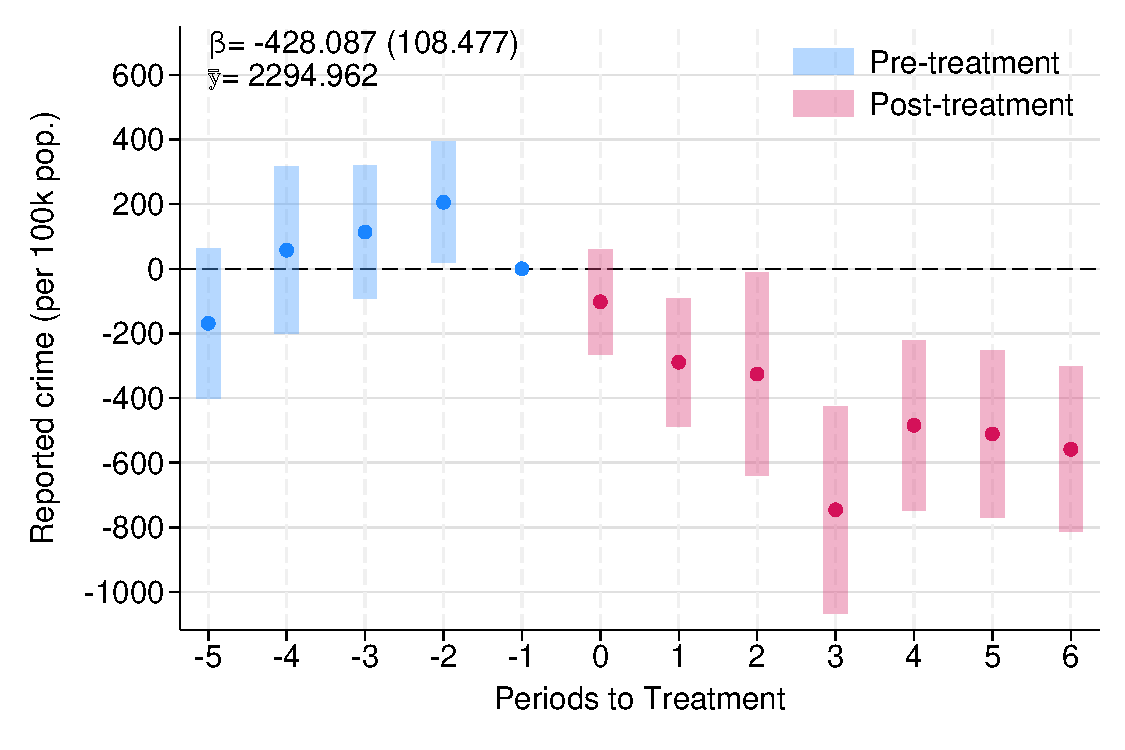
\includegraphics[width=\textwidth]{../manuscript/Graphs/totalreportedcrime_47enusc.pdf}
        \caption{Reported crime per 100k inhabitants}
    \end{subfigure}%
    ~ 
    \begin{subfigure}{0.495\textwidth}
    \centering
    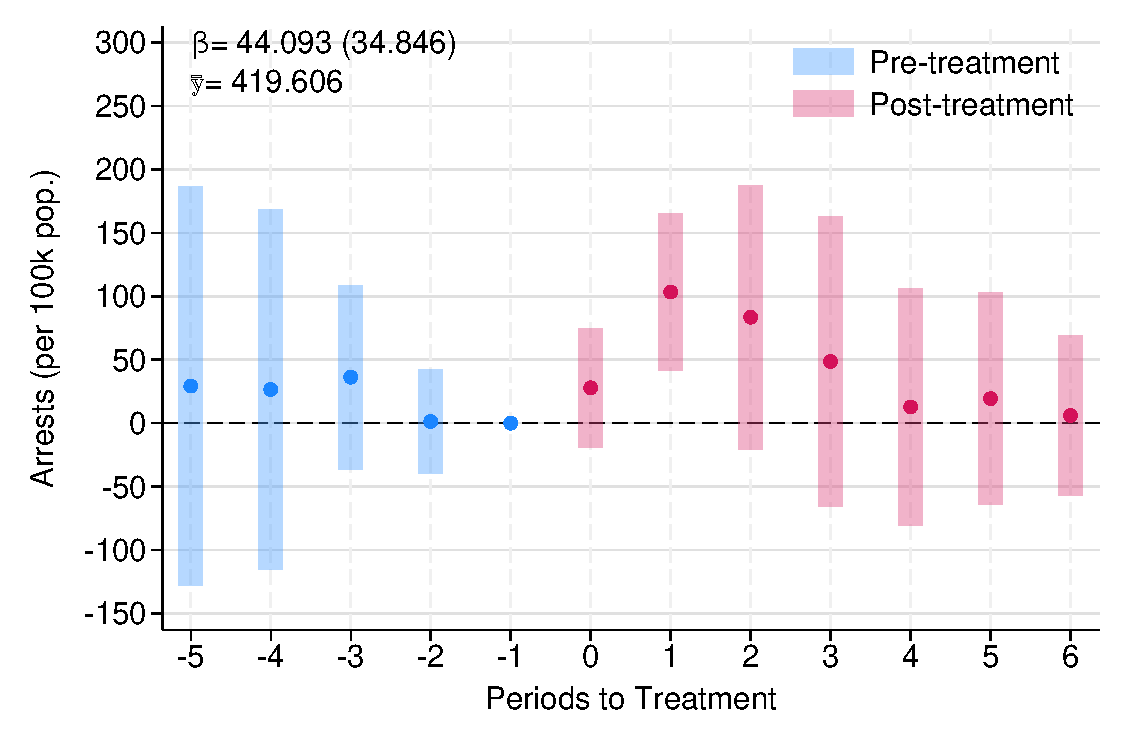
\includegraphics[width=\textwidth]{../manuscript/Graphs/totalarrestscrime_47enusc.pdf}
        \caption{Arrests per 100k inhabitants}
    \end{subfigure}
    \\[12pt]
    \begin{minipage}{0.99\textwidth}
    \footnotesize Notes: This figure shows the dynamic effects of \emph{Plan Cuadrante} on the number of crimes reported to the police per 100,000 inhabitants in the municipality in panel (a) and on the number of arrests per 100,000 inhabitants in the municipality in panel (b) using administrative data from the Undersecretary for Crime Prevention. The analysis is conducted using only the sample of municipalities included in the analysis of ENUSC outcomes. Panel (a) includes 592 observations, while panel (b) includes 405 observations. The estimation is conducted using the procedure developed in \citet{Callaway} for difference-in-differences with staggered treatment adoption. The dots in the figure represent the estimated coefficients and the bars behind them 95\% confidence intervals. Standard errors are clustered at the municipality level using wild bootstrapping. The pooled effect and the mean outcome before the introduction of the treatment is also presented in each panel. 
    \end{minipage}
\end{figure}
}

\clearpage
\end{response}
\stepcounter{AnsweredComments}


% Comment R2 - 12
\begin{refcomment}

Minor Comments:

1.	There is an additional period (.) after footnote 9.

\label{pt:r2_12}
\end{refcomment}

\begin{response}
    %Minor Comments:

%1.	There is an additional period (.) after footnote 9.

Thanks. This is corrected in the updated version of the manuscript.



\end{response}
\stepcounter{AnsweredComments}



% Comment R2 - 13
\begin{refcomment}

2.	Add space before “Using a difference-in-differences specification...” on page 11.

\label{pt:r2_13}
\end{refcomment}

\begin{response}
    %2.	Add space before “Using a difference-in-differences specification...” on page 11.

Thanks. This is now corrected in the updated manuscript.

\end{response}
\stepcounter{AnsweredComments}



% Comment R2 - 14
\begin{refcomment}

3. Notes on Figure 4 are missing the word “observations” after “This panel includes 8,495, 7,975, 8,326, 7,439, 6,621, 7,712, 7,889”
\label{pt:r2_14}
\end{refcomment}

\begin{response}
    %3.	Notes on Figure 4 are missing the word “observations” after “This panel includes 8,495, 7,975, 8,326, 7,439, 6,621, 7,712, 7,889”

Thanks. This is corrected in the updated manuscript.

\clearpage
\noindent\textbf{Other figure referenced above:}
\vspace{0.5em}

{\setcounter{figure}{3}\renewcommand{\thefigure}{\arabic{figure}}
%--- Implementation
\begin{figure}[!ht]
    \centering
    \caption[\emph{Plan Cuadrante} and Changes in Police Performance]{\emph{Plan Cuadrante} and Changes in Police Performance}
    \label{fig:figure05}
    \label{fig:police_performance}
    \label{fig:effectiveness_es}
    \begin{subfigure}[t]{0.44\textwidth}
        \centering
        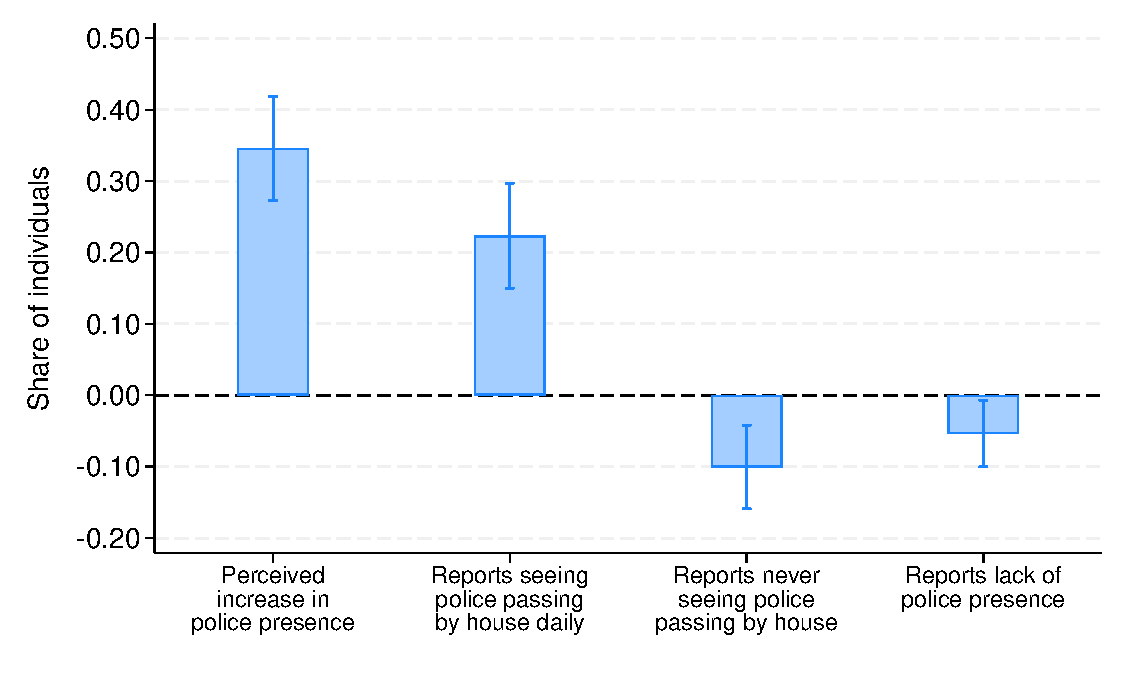
\includegraphics[width=\linewidth]{../manuscript/Graphs/results_policepresence.pdf}
        \caption{Effect on police presence}
    \end{subfigure}\hfill
    \begin{subfigure}[t]{0.44\textwidth}
        \centering
        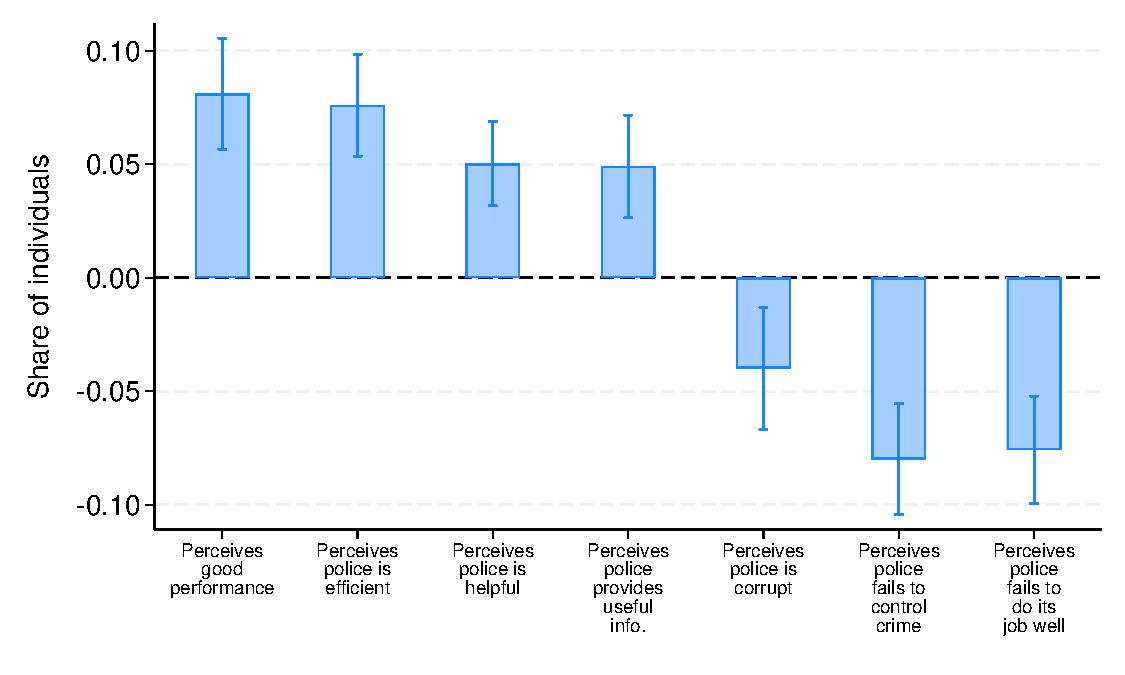
\includegraphics[width=\linewidth]{../manuscript/Graphs/combined_PCttest_2.pdf}
        \caption{Effect on perceived police performance}
    \end{subfigure}
    \\[6pt]
    \begin{subfigure}[t]{0.44\textwidth}
        \centering
        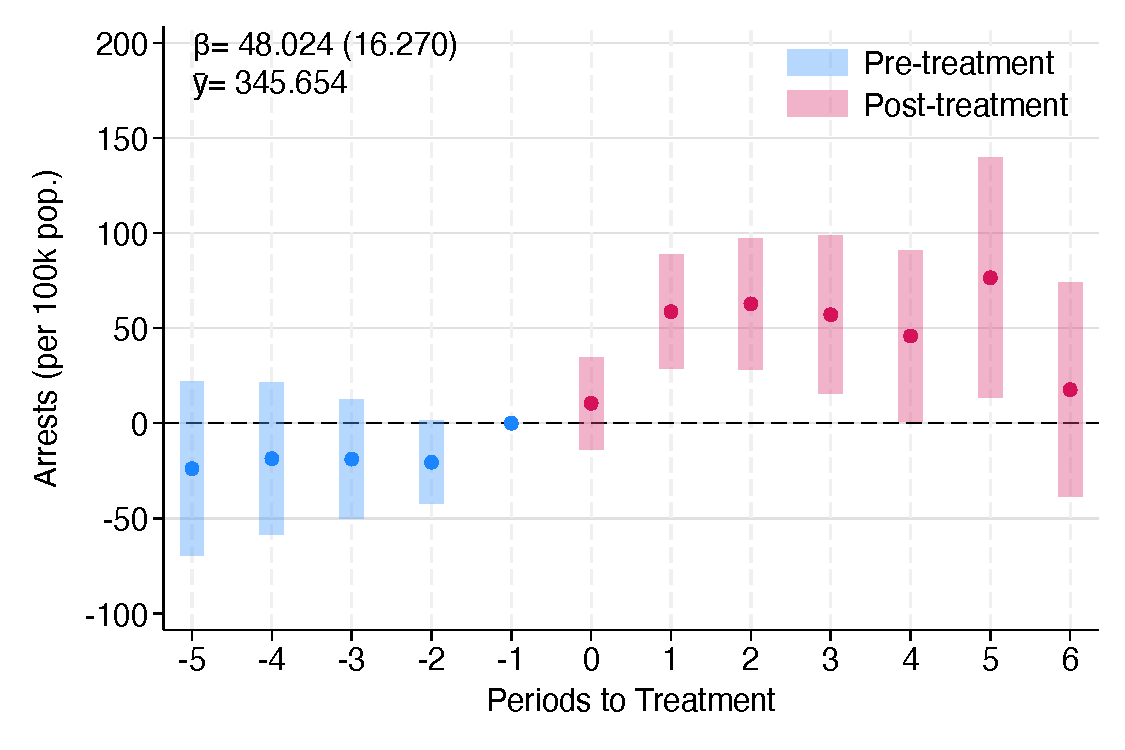
\includegraphics[width=\linewidth]{../manuscript/Graphs/totalarrestscrime_allcomunas.pdf}
        \caption{Arrests (per 100k pop.)}
    \end{subfigure}\hfill
    \begin{subfigure}[t]{0.44\textwidth}
        \centering
        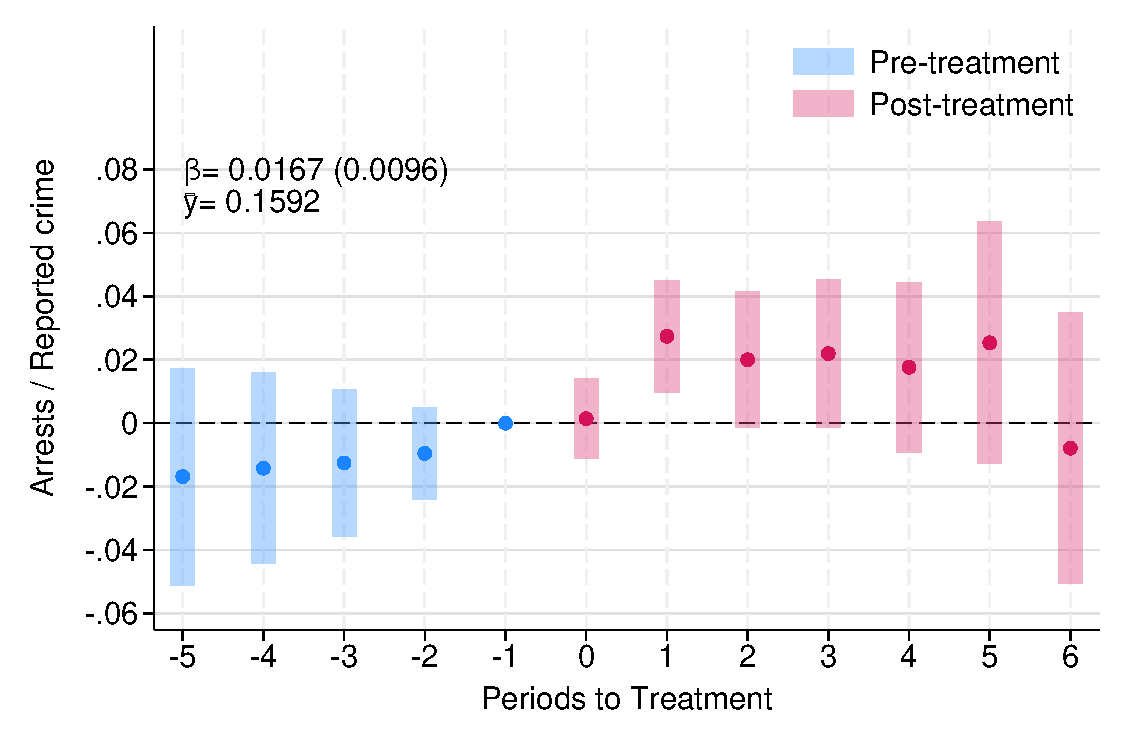
\includegraphics[width=\linewidth]{../manuscript/Graphs/arrests_over_reportedcrime_allcomunas.pdf}
        \caption{Arrests / Reported crime}
    \end{subfigure}
    \\[6pt]
    \begin{subfigure}[t]{0.44\textwidth}
        \centering
        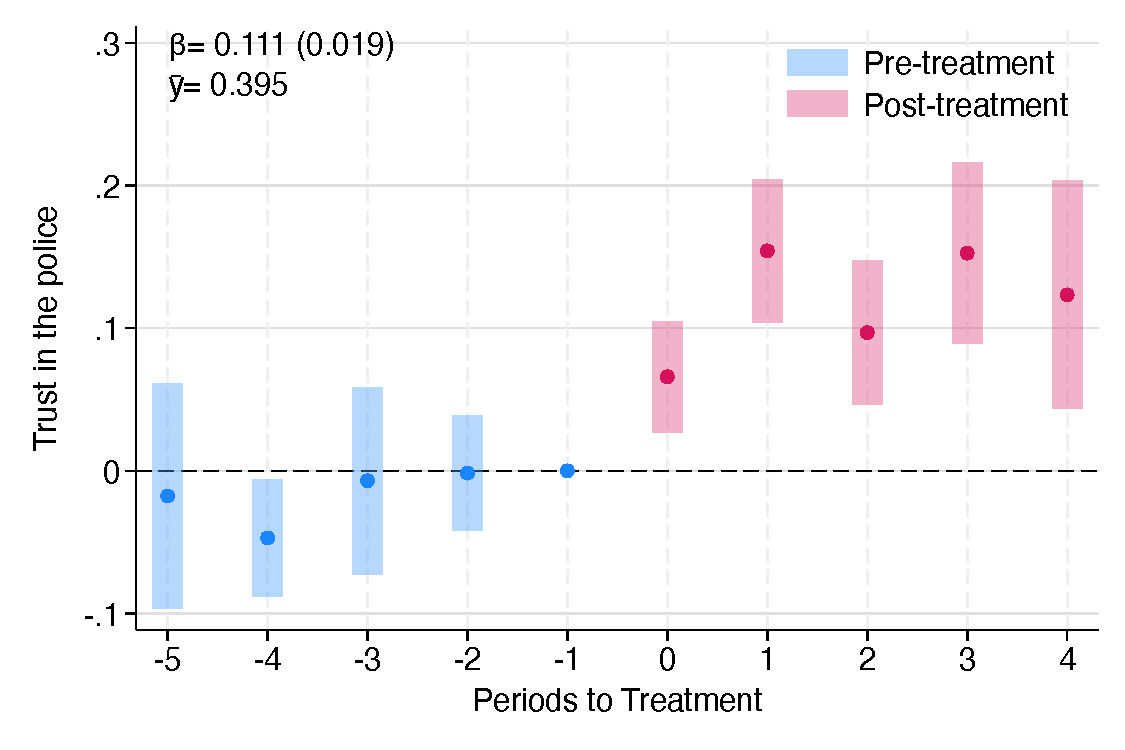
\includegraphics[width=\linewidth]{../manuscript/Graphs/results_trustcarabineros.pdf}
        \caption{Trust in the police}
    \end{subfigure}
    \\[8pt]
    \begin{minipage}{0.99\textwidth}
    \footnotesize Notes: Panel (a) reports the effects on perceived police presence. Panel (b) reports perceived police performance in 2005, comparing municipalities where \emph{Plan Cuadrante} was already implemented before 2006 with municipalities where it was implemented after 2005. Panels (c), (d), and (e) report dynamic event-study estimates for arrests per 100,000 inhabitants, the ratio of arrests to reported crime, and trust in the police. The estimation follows \citet{Callaway}. The graphs display estimated coefficients and 95\% confidence intervals. Standard errors are clustered at the municipality level using the wild bootstrapping procedure.
    \end{minipage}
\end{figure}
}

\clearpage
\end{response}
\stepcounter{AnsweredComments}

% Comment R2 - 15
\begin{refcomment}

4. Sometimes the authors use the word “Police” and others they use the word “Carabineros” (e.g., Panel a of Figure 4), I suggest sticking to one.

\label{pt:r2_15}
\end{refcomment}

\begin{response}
    %4.	Sometimes the authors use the word “Police” and others they use the word “Carabineros” (e.g., Panel a of Figure 4), I suggest sticking to one.

Thanks. In the updated version of the manuscript, we restrict the use of the term "Carabineros" only to the description of the institution.



\end{response}
\stepcounter{AnsweredComments}

\putbib
\end{bibunit}